% !TEX program = xelatex
\documentclass[UTF8,fontset=fandol,a4paper,11pt]{ctexart}
\usepackage[margin=21mm,top=23mm,bottom=22mm,headheight=16pt]{geometry}
\usepackage{amsmath,amssymb,mathtools,bm}
\usepackage{tikz}
\usetikzlibrary{arrows.meta,calc,angles,quotes,patterns,decorations.pathmorphing}
\usepackage{xcolor,booktabs,array,longtable,enumitem,fancyhdr,needspace}
\usepackage[unicode,hidelinks]{hyperref}
\definecolor{ink}{HTML}{24343C}
\definecolor{accent}{HTML}{166A70}
\definecolor{muted}{HTML}{65747A}
\definecolor{rulegray}{HTML}{D4DDE0}
\definecolor{warm}{HTML}{966037}
\color{ink}
\setlength{\parindent}{2em}
\setlength{\parskip}{4pt}
\linespread{1.12}
\AtBeginDocument{\setlength{\abovedisplayskip}{6pt plus 2pt minus 1pt}
\setlength{\belowdisplayskip}{6pt plus 2pt minus 1pt}
\setlength{\abovedisplayshortskip}{0pt plus 1pt}
\setlength{\belowdisplayshortskip}{4pt plus 1pt}}
\setlist[enumerate]{label=(\arabic*),leftmargin=2.3em,itemsep=3pt,topsep=4pt}
\setlist[itemize]{leftmargin=2em,itemsep=2pt,topsep=4pt}
\allowdisplaybreaks[1]
\setlength{\emergencystretch}{2em}
\setcounter{secnumdepth}{0}
\providecommand{\tightlist}{\setlength{\itemsep}{0pt}\setlength{\parskip}{0pt}}
\ctexset{section={format=\Large\bfseries\color{accent},beforeskip=10pt,afterskip=9pt},
subsection={format=\normalsize\bfseries\color{accent},beforeskip=10pt,afterskip=4pt},
subsubsection={format=\normalsize\bfseries,beforeskip=8pt,afterskip=3pt}}
\pagestyle{fancy}
\fancyhf{}
\fancyhead[L]{\small\color{muted}物理学难题集萃}
% 页眉仅保留书名；版本名称只在封面显示。
\fancyfoot[L]{\small\color{muted}\chapterlabel}
\fancyfoot[R]{\small\thepage}
\renewcommand{\headrulewidth}{0.4pt}
\renewcommand{\footrulewidth}{0pt}
\newcommand{\dd}{\mathop{}\!\mathrm{d}}
\newcommand{\vect}[1]{\bm{#1}}
\newcommand{\tagline}[1]{\noindent{\small\color{muted}#1}\par}
\newcommand{\result}[1]{\begin{equation*}\boxed{#1}\end{equation*}}
\newcommand{\figcaption}[1]{\par\vspace{2pt}{\small\color{muted}#1}\par}
\newcommand{\teach}[2]{\Needspace{4\baselineskip}\subsection*{讲解要点与追问}#1\par\smallskip\noindent\textbf{追问：}#2\par}
\newcommand{\workarea}{\par\vspace{7mm}\noindent{\small\color{muted}作答区}\par\vspace{4mm}
\noindent\textcolor{rulegray}{\rule{\linewidth}{0.3pt}}\par\vspace{16mm}
\noindent\textcolor{rulegray}{\rule{\linewidth}{0.3pt}}\par\vspace{16mm}
\noindent\textcolor{rulegray}{\rule{\linewidth}{0.3pt}}\par\vspace{16mm}
\noindent\textcolor{rulegray}{\rule{\linewidth}{0.3pt}}}
\tikzset{axis/.style={-{Stealth[length=2mm]},thin,color=muted},
motion/.style={-{Stealth[length=2.3mm]},thick,color=accent},
force/.style={-{Stealth[length=2.3mm]},thick,color=warm},
traj/.style={thick,color=accent},guide/.style={dashed,thin,color=muted},
object/.style={thick,color=ink},every node/.style={font=\small}}\widowpenalty=10000\clubpenalty=10000\displaywidowpenalty=10000

\newcommand{\chapterlabel}{第五章\quad 静力平衡}
\hypersetup{pdftitle={第五章 静力平衡·教师版},pdfauthor={},pdfsubject={第五章第1--12题}}
\begin{document}
\pdfbookmark[0]{第五章 静力平衡}{cover}
\thispagestyle{empty}
\vspace*{20mm}
\noindent{\Huge\bfseries 物理学难题集萃}\par\vspace{8mm}
\noindent{\LARGE 第五章\quad 静力平衡}\par\vspace{10mm}
\noindent{\Large\color{accent}教师版}\par\vspace{8mm}
\noindent\textcolor{accent}{\rule{\linewidth}{1pt}}\par\vspace{8mm}
\noindent 第 1--12 题\par\vspace{5mm}
\noindent 详细解答、备课分析、课堂追问与变式训练。\par
\vfill\clearpage
\pdfbookmark[1]{题目目录}{contents}
\section*{题目目录}
\begin{longtable}{@{}>{\color{accent}\bfseries}r p{120mm}@{}}
\toprule 题号 & 题目\\\midrule
1 & 圆锥面上链环的张力 \\
2 & 水平杆靠墙的摩擦条件 \\
3 & 竖杆受水平力的防滑条件 \\
4 & 半球凹面内的均匀细杆 \\
5 & 三圆柱堆放的摩擦下限 \\
6 & 斜木板上三球的支承 \\
7 & 分段悬线的平衡与提升功 \\
8 & 浮子与插杆的稳定性 \\
9 & 五杆悬挂的平衡形状 \\
10 & 厚木板在圆柱上的稳定性 \\
11 & 菱形木条与圆盘的平衡 \\
12 & 细绳张力与悬链线 \\
\bottomrule\end{longtable}


\clearpage

\pdfbookmark[2]{第 1 题 圆锥面上链环的张力}{q1}

\section*{第 1 题\quad 圆锥面上链环的张力}

\tagline{M-05-01}

顶角为 $\alpha$ 的圆锥体竖直固定，顶点在上。质量为 $m$、质量分布均匀的链环水平套在圆锥面上，处于静止状态。忽略链环与圆锥面之间的摩擦，$0<\alpha<\pi$。求链环中的张力。

\begin{center}\begin{minipage}{\linewidth}\centering
\begin{tikzpicture}
\draw[object] (-2,0)--(0,4)--(2,0);\draw[guide] (0,0)--(0,4);\draw[object] (0,1.6) ellipse (1.2 and .32);\draw (0,3.3) arc(-90:-116.57:.7);\node at (-.45,3.15) {$\alpha/2$};\node[right] at (1.3,1.6) {$m$};\node[below] at (0,-.1) {链环水平};
\end{tikzpicture}
\figcaption{图 5.1\quad 水平链环套在圆锥外侧，锥面母线与竖直轴夹角为 $\alpha/2$。}
\end{minipage}\end{center}

\Needspace{5\baselineskip}

\pdfbookmark[3]{题型定位}{q1-h0}

\subsection*{题型定位}

弯曲柔性体的微元平衡。整环的外力平衡只能给总支持力，内部张力要通过切开的链元确定。等大张力因方向不同留下径向合力，与圆锥支持力的水平分量平衡。

可用本题从离散物体过渡到连续绳链：先分别观察截面和俯视受力，再以张角表示微元质量。后面的悬链线题仍沿用张力大小及方向共同变化的处理。

\Needspace{5\baselineskip}

\pdfbookmark[3]{知识点}{q1-h1}

\subsection*{知识点}

\begin{itemize}
\tightlist
\item
  链元微元平衡
\item
  圆锥面法向支持力分解
\item
  张力方向变化形成合力
\item
  小角近似 \(\sin(\Delta\varphi/2)\approx\Delta\varphi/2\)
\item
  线密度与张角对应关系
\end{itemize}

圆环微元两端张力的合力指向局部曲率中心，大小一阶正比微元转角。锥面支持力的竖直分量平衡重量，水平分量与张力合力平衡。微元质量按弧长取值。给定整环质量时半径$r$约去，重力加速度$g$保留；若给固定线密度，张力还与$r$成正比。解图5.1B的有限弧支持力沿弧改变方向，须积分其投影。


\Needspace{5\baselineskip}

\pdfbookmark[3]{物理图像}{q1-h2}

\subsection*{物理图像}

解图5.1A的支持力沿锥面外法线，竖直分量向上，水平分量朝外。链环两端的张力沿切线，合力却朝圆心，恰好抵消支持力的水平分量。

放大链元时，应同时看两个投影：子午截面显示重力与支持力的分解，俯视图显示两端切线方向的变化。整环的水平外力因对称相消，但局部链元仍需张力维持曲率。

\Needspace{5\baselineskip}

\pdfbookmark[3]{解题入口}{q1-h3}

\subsection*{解题入口}

取圆心角 $\dd\varphi$ 的链元，先用竖直平衡 $N\sin(\alpha/2)=\dd m\,g$，再用径向平衡 $T\dd\varphi=N\cos(\alpha/2)$。均匀分布给出 $\dd m=m\dd\varphi/(2\pi)$，消去支持力与张角。

板书应保留有限小角的 $2T\sin(\Delta\varphi/2)$ 到微元 $T\dd\varphi$ 的过渡，并说明分布支持力也只保留同阶项。这样不会把有限弧的合力与微元式混用。

\Needspace{5\baselineskip}

\pdfbookmark[3]{标准解法}{q1-h4}

\subsection*{标准解法}

\textbf{链元的质量与支持力。}整环的水平支持力相互抵消。截取链弧后，切口处的张力成为该段外力，才能由受力求得。取对应圆心角 $\dd\varphi$ 的短链元。设链环半径为 $r$，质量均匀，故
\[
 \dd s=r\dd\varphi,\qquad
 \dd m=\frac{m}{2\pi r}\dd s=\frac{m}{2\pi}\dd\varphi.
\]
记圆锥半顶角为 $\beta=\alpha/2$。解图5.1A中，支持力 $N$ 垂直于锥面，方向朝外且向上。其竖直分量承受链元重力：
\[
 N\sin\beta=\dd m\,g,
 \qquad N=\frac{mg}{2\pi\sin\beta}\dd\varphi.
\]
\begin{center}\begin{minipage}{\linewidth}\centering
\begin{tikzpicture}
\draw[object](-1.5,0)--(0,3)--(1.5,0);
\coordinate(P)at(.85,1.3);\fill(P)circle(2pt)node[below left]{$P$};
\draw[force](P)--(2.4,2.075)node[above]{$N$};
\draw[guide](P)--(2.4,1.3)--(2.4,2.075);
\node[below]at(1.7,1.3){$N_r$};\node[right]at(2.4,1.7){$N_z$};
\draw[force](P)--(.85,.525)node[below]{$\dd m\,g$};
\draw[force](P)--(-.7,1.3)node[midway,above]{$T\,\dd\varphi$};
\node[align=left,anchor=west]at(3.3,2){$N_r=T\,\dd\varphi$\\$N_z=\dd m\,g$\\法向力垂直锥面};
\end{tikzpicture}
\figcaption{解图5.1A\quad 子午截面的微元受力；各方向合力分别平衡，支持力朝外且向上。}
\end{minipage}\end{center}
\textbf{张力合力来自方向的变化。}解图5.1B的两端张力大小相等，沿链环切线。若先取一个小而有限的圆心角 $\Delta\varphi$，两张力的合力大小为 $2T\sin(\Delta\varphi/2)$，方向指向圆心。分布支持力也须沿弧积分；在 $\Delta\varphi\to0$ 的一阶近似下，其水平合力为 $N\cos\beta$。因此微元径向平衡为
\[
 T\dd\varphi=N\cos\beta.
\]
\begin{center}\begin{minipage}{\linewidth}\centering
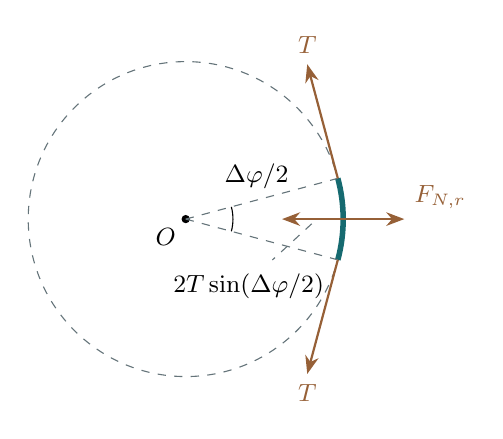
\begin{tikzpicture}
\draw[guide](0,0)circle(2);\fill(0,0)circle(1.5pt)node[below left]{$O$};
\draw[traj,line width=2pt](-15:2)arc(-15:15:2);
\draw[guide](0,0)--(-15:2);\draw[guide](0,0)--(15:2);
\draw[force](15:2)--++(-.388228568,1.448888739)node[above]{$T$};
\draw[force](-15:2)--++(-.388228568,-1.448888739)node[below]{$T$};
\draw[force](2,0)--(2.776457135,0)node[above right]{$F_{N,r}$};
\draw[force](2,0)--(1.223542865,0);
\draw[guide](1.6,-.06)--(1.1,-.52);
\node at(.8,-.85){$2T\sin(\Delta\varphi/2)$};
\draw(.6,0)arc(0:15:.6);\draw(.6,0)arc(0:-15:.6);
\node at(.9,.55){$\Delta\varphi/2$};
\end{tikzpicture}
\figcaption{解图5.1B\quad 有限链弧的俯视图；两端张力沿切线，分布支持力的水平合力须逐段投影。}
\end{minipage}\end{center}
消去 $N$ 和 $\dd\varphi$，得到
\[
 T=\frac{mg}{2\pi}\frac{\cos\beta}{\sin\beta},
\qquad
 \boxed{T=\frac{mg}{2\pi\tan(\alpha/2)}}.
\]
两端张力沿不同切线，其径向分量相加，留下与弧长同阶的向内合力。

\textbf{环半径与锥顶角对张力的影响。}半径 $r$ 约去，是因为同一质量的环越大，单位弧长越轻，同时曲率越小，两者在微元方程中抵消。$\alpha\to0$ 时，锥面接近竖直，支持力的竖直分量很小，所需张力趋于无穷；$\alpha\to\pi$ 时，锥面接近水平，张力趋于零。这些是 $0<\alpha<\pi$ 的锥面接触构型分别趋近两端时的极限。
\subsubsection*{有限弧的张力和支持力}
解图5.1B把短弧画成以正径向为对称轴、两端极角为$\pm\Delta\varphi/2$的有限弧。
令$\lambda=m/(2\pi r)$。在极角$\psi$处，
小段重力为$\lambda gr\,\dd\psi$，竖直平衡给
\[
\dd N\sin\beta=\lambda gr\,\dd\psi.
\]
各段支持力的水平分量沿各处的径向。取有限弧的对称轴为基准，沿轴分量由 $\dd N\cos\beta$ 再乘 $\cos\psi$ 得到。垂直于轴的分量关于对称轴相消：
\[
\begin{aligned}
F_{N,r}
&=\int_{-\Delta\varphi/2}^{\Delta\varphi/2}
\cos\beta\cos\psi\,\dd N\\
&=\lambda gr\cot\beta
\int_{-\Delta\varphi/2}^{\Delta\varphi/2}\cos\psi\,\dd\psi\\
&=2\lambda gr\cot\beta\sin\frac{\Delta\varphi}2.
\end{aligned}
\]
两端张力沿各自切线，其沿对称轴的合力为
$2T\sin(\Delta\varphi/2)$，方向与$F_{N,r}$相反。
取$0<\Delta\varphi<2\pi$，约去非零的正弦因子，仍得
\[
T=\lambda gr\cot\beta=\frac{mg}{2\pi}\cot\beta.
\]
有限弧积分与微元平衡给出同一个张力。取整环时 $\Delta\varphi=2\pi$，两种水平合力都为零，径向合力式成为 $0=0$，张力要由截取的弧段确定。

单位弧长的曲率平衡还可写为
\[
\frac Tr=\lambda g\cot\beta,\qquad
\frac{\dd N}{\dd s}=\frac{\lambda g}{\sin\beta}.
\]
左式中 $T/r$ 是张力方向沿弧改变时产生的向内合力密度。右式是沿锥面外法线的支持力密度，其径向分量为 $(\dd N/\dd s)\cos\beta$。
把$\lambda=m/(2\pi r)$代入才会约去$r$；
若已知的是固定线密度，张力便随环半径增加。
重力加速度$g$没有约去，重力越强、同一几何所需张力越大。
在$0<\beta<\pi/2$时$N,T$均为正，分别符合单侧支持与链条只能受拉的条件。


\Needspace{5\baselineskip}

\pdfbookmark[3]{关键洞察}{q1-h5}

\subsection*{关键洞察}

解图5.1B中两端切线方向不同，留下向内合力；有限弧的支持力也须逐段投影，积分后与端张力同含$2\sin(\Delta\varphi/2)$因子。给定整环质量时半径约去，给固定线密度时则保留$r$；重力加速度$g$始终保留。

\Needspace{5\baselineskip}

\pdfbookmark[3]{易错点}{q1-h6}

\subsection*{易错点}

\begin{itemize}\item 支持力的水平分量朝外，张力合力朝内，两项在径向平衡。\item 锥面与轴线夹角为 $\alpha/2$，竖直分量是 $N\sin(\alpha/2)$。\item 两端张力向对称轴的投影各为$T\sin(\Delta\varphi/2)$，合量为$2T\sin(\Delta\varphi/2)$。\item 链元质量是$m\Delta\varphi/(2\pi)$，由线密度乘弧长得到，半径在这两项中约去。\item 微元式取转角趋零的一阶项，有限弧的支持力沿各处法线投影后积分。\end{itemize}

\Needspace{5\baselineskip}

\pdfbookmark[3]{课堂讲解建议}{q1-h7}

\subsection*{课堂讲解建议}

先让学生在解图5.1B的两个端点画切线方向，说明两张力的合力为什么朝内。再到解图5.1A判断锥面支持力朝外，两个图的径向方向一致后才写方程。板书保留链元质量、竖直平衡和径向平衡三行，展示同一个张角如何约去。

把锥面逐渐放平，问“支持力的水平分量怎样变？”学生从截面图读出水平分量减小，再由径向平衡说明张力降低。接着分别给定整环质量和线密度，让学生写出链元质量，说明前一种输入中$r$约去，后一种保留$r$。再指向悬链线微元，比较两端切向张力怎样随曲线方向转动，并用法向平衡联系曲率。

再取一个有限弧，问“各段水平支持力沿同一方向吗？”让学生把各段法线投影到弧的对称轴，写出额外的$\cos\psi$。
由$\int\cos\psi\,\dd\psi$得到与端张力相同的$2\sin(\Delta\varphi/2)$因子，
再问整环为什么退化为$0=0$。这能区分“微元式正确”与“把有限分布力全部集中”两种做法。

\Needspace{5\baselineskip}

\pdfbookmark[3]{变式训练}{q1-h8}

\subsection*{变式训练}

\begin{enumerate}
\item 将圆锥换成外侧光滑半球面。纬线的极角 $\psi$ 是球心至链环的半径与竖直向上的夹角，$0<\psi<\pi/2$。变图5.1V1 的支持力沿半径，故$N\cos\psi=\dd m\,g$、$T\dd\varphi=N\sin\psi$。用$\dd m=m\dd\varphi/(2\pi)$，消去$N$：
\[
T=\frac{mg}{2\pi}\tan\psi.
\]
纬线趋于球顶时支持力几乎竖直，张力趋零；趋向赤道时其竖直分量趋零，所需张力发散。
\begin{center}\begin{minipage}{.98\linewidth}\centering
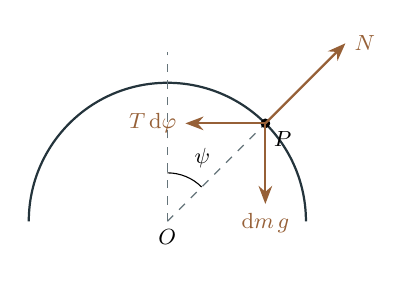
\begin{tikzpicture}[scale=.88,transform shape]
\draw[object] (-2,0) arc(180:0:2);
\draw[guide] (0,0)--(0,2.45);
\draw[guide] (0,0)--(1.4142,1.4142);
\fill (1.4142,1.4142) circle(2pt) node[below right] {$P$};
\draw[force] (1.4142,1.4142)--(2.57,2.57) node[right] {$N$};
\draw[force] (1.4142,1.4142)--(1.4142,.25) node[below] {$\dd m\,g$};
\draw[force] (1.4142,1.4142)--(.26,1.4142) node[left] {$T\dd\varphi$};
\draw (0,.7) arc(90:45:.7) node[midway,above right] {$\psi$};
\node[below] at (0,0) {$O$};
\end{tikzpicture}
\figcaption{变图5.1V1\quad 上半球外侧的支持力沿半径向外，竖直分量为正。}
\end{minipage}\end{center}
\item 换成质量$m_a$、圆心角$\eta$的均匀圆弧，求端力。单位角质量为$m_a/\eta$，微元平衡给$T=m_ag\cot\beta/\eta$，$\beta=\alpha/2$。变图5.1V2 两端切向外力各为$T$，垂直弧对称轴的分量相消，径向分量相加，合力为$2T\sin(\eta/2)$。支持力沿弧投影积分：
\[
F_{N,r}=\frac{m_ag}{\eta}\cot\beta\int_{-\eta/2}^{\eta/2}\cos\varphi\,\dd\varphi
=2T\sin(\eta/2).
\]
这给出整段弧的外力平衡和每个切口的力。
\begin{center}\begin{minipage}{.98\linewidth}\centering
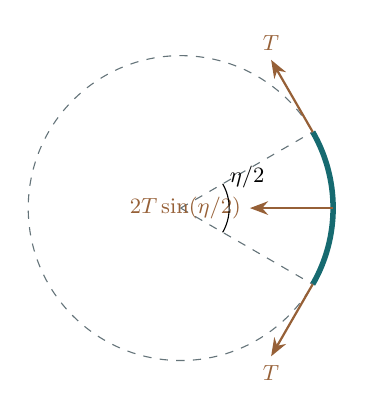
\begin{tikzpicture}[scale=.88,transform shape]
\draw[guide] (0,0) circle(2.2);
\draw[traj,line width=2pt] (-30:2.2) arc(-30:30:2.2);
\draw[guide] (0,0)--(-30:2.2); \draw[guide] (0,0)--(30:2.2);
\draw[force] (30:2.2)--++(-.6,1.03923) node[above] {$T$};
\draw[force] (-30:2.2)--++(-.6,-1.03923) node[below] {$T$};
\draw[force] (2.2,0)--(1,0) node[left] {$2T\sin(\eta/2)$};
\draw (.7,0) arc(0:30:.7); \draw (.7,0) arc(0:-30:.7);
\node at (.96,.45) {$\eta/2$};
\end{tikzpicture}
\figcaption{变图5.1V2\quad 取 $\eta=60^\circ$ 示两切口的张力及其向内合力。}
\end{minipage}\end{center}
\item 用角度极限判张力趋势。变图5.1V3 的纵坐标是$\cot\beta$。$\beta\to0$时$\sin\beta\sim\beta$，支持力$N=\dd m\,g/\sin\beta$增大，张力$T\sim mg/(2\pi\beta)$。$\beta\to\pi/2$时令$\varepsilon=\pi/2-\beta$，有$T\sim mg\varepsilon/(2\pi)$，趋零。这些是非退化锥面$0<\beta<\pi/2$的两端极限。
\begin{center}\begin{minipage}{.98\linewidth}\centering
\begin{tikzpicture}[scale=.88,transform shape]
\draw[axis] (0,0)--(6.65,0) node[right] {$\beta$};
\draw[axis] (0,0)--(0,4.3) node[above] {$2\pi T/(mg)$};
\draw[traj,domain=15:85,samples=100] plot({\x/15},{1/tan(\x)});
\fill (3,1) circle(1.6pt) node[above right] {$(45^\circ,1)$};
\node[below] at (6,0) {$90^\circ$};
\end{tikzpicture}
\figcaption{变图5.1V3\quad 无摩擦时的张力随半顶角增加而降低。}
\end{minipage}\end{center}
\item 沿母线有静摩擦，求允许张力。变图5.1V4 取向上、向内的摩擦$f$为正。平衡给$N\sin\beta+f\cos\beta=\dd m\,g$、$N\cos\beta-f\sin\beta=T\dd\varphi$。令$q=f/N$，有
\[
T=\frac{mg}{2\pi}\frac{\cos\beta-q\sin\beta}{\sin\beta+q\cos\beta},
\qquad |q|\le\mu.
\]
取支持力和张力非负，即分母为正、分子非负。若$\mu<\min(\tan\beta,\cot\beta)$，整个$q\in[-\mu,\mu]$都允许；右侧比值对$q$的导数为$-1/(\sin\beta+q\cos\beta)^2$，因此上下限分别在$q=-\mu,+\mu$取得。若给出的 $\mu$ 较大，先取 $q\in[-\mu,\mu]\cap(-\tan\beta,\cot\beta]$，再用上式的单调性读两端。$\mu\ge\cot\beta$ 时，最小值为零，母线静摩擦与支持力可直接平衡重力；$\mu\ge\tan\beta$ 时，$q$ 从右侧趋向 $-\tan\beta$，分母趋零而分子保持为正，理想模型中的张力无有限上限。
\begin{center}\begin{minipage}{.98\linewidth}\centering
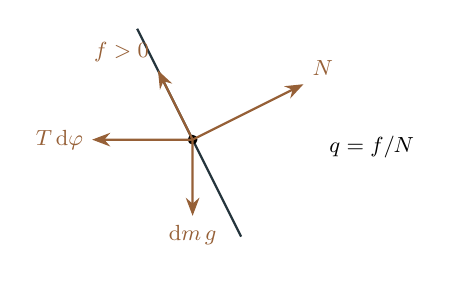
\begin{tikzpicture}[scale=.88,transform shape]
\draw[object] (0,3)--(1.5,0);
\coordinate(P) at (.8,1.4);
\fill(P)circle(2pt);
\draw[force](P)--(2.4,2.2) node[above right] {$N$};
\draw[force](P)--(.3,2.4) node[above left] {$f>0$};
\draw[force](P)--(.8,.3) node[below] {$\dd m\,g$};
\draw[force](P)--(-.65,1.4) node[left] {$T\dd\varphi$};
\node[right] at (2.65,1.3) {$q=f/N$};
\end{tikzpicture}
\figcaption{变图5.1V4\quad 取沿母线向上、向内的摩擦为正，法线与切线分量分别投影。}
\end{minipage}\end{center}
\item 完整环切去小缺口，剩弧保持$r,\lambda$，求两端所需外力。变图5.1V5 两切口外力沿切线。取任一内段$r\dd\varphi$，支持力的径向分量为$\lambda gr\cot\beta\,\dd\varphi$，张力合力为$T\dd\varphi$，故$T=\lambda gr\cot\beta$。缺口改变剩余总质量，局部线密度和曲率则仍给同一张力。若固定的是剩弧质量$m_a$与弧角$\eta$，用$\lambda r=m_a/\eta$即得变图5.1V2 的结果。
\begin{center}\begin{minipage}{.98\linewidth}\centering
\begin{tikzpicture}[scale=.88,transform shape]
\draw[traj,line width=1.4pt] (18:2) arc(18:342:2);
\draw[force] (18:2)--++(-.3708,1.1413) node[above] {$T$};
\draw[force] (342:2)--++(-.3708,-1.1413) node[below] {$T$};
\draw[guide] (0,0)--(18:2); \draw[guide] (0,0)--(342:2);
\node at (2.6,0) {缺口}; \node at (-.1,0) {$r$};
\end{tikzpicture}
\figcaption{变图5.1V5\quad 切去缺口后，剩弧的两个端力沿端点切线显露。}
\end{minipage}\end{center}
\item 链环可承受的最大张力为$T_{\max}$，求最大质量。由$T=mg\cot\beta/(2\pi)$及$T\le T_{\max}$，得
\[
m_{\max}=\frac{2\pi T_{\max}}g\tan\beta.
\]
变图5.1V6 给出张力强度决定的质量上限。该状态各段还需承担法向力密度$\lambda g/\sin\beta$；若支持面的承载能力也有给定上限，把这项局部法向载荷一并代入比较。
\begin{center}\begin{minipage}{.98\linewidth}\centering
\begin{tikzpicture}[scale=.88,transform shape]
\draw[axis] (0,0)--(6.45,0) node[right] {$\beta$};
\draw[axis] (0,0)--(0,4.0) node[above] {$m_{\max}g/(2\pi T_{\max})$};
\draw[traj,domain=0:75,samples=100] plot({\x/15},{tan(\x)});
\fill (3,1) circle(1.6pt) node[right] {$(45^\circ,1)$};
\node[below] at (5,0) {$75^\circ$};
\end{tikzpicture}
\figcaption{变图5.1V6\quad 在给定链条最大张力下，最大质量随半顶角增大。}
\end{minipage}\end{center}\end{enumerate}

\clearpage

\pdfbookmark[2]{第 2 题 水平杆靠墙的摩擦条件}{q2}

\section*{第 2 题\quad 水平杆靠墙的摩擦条件}

\tagline{M-05-02}

均匀杆 $AB$ 长为 $l$，重量为 $w_0$。$A$ 端接触粗糙竖直墙，$B$ 端用不可伸长的轻绳悬于墙上的 $C$ 点。杆水平，绳与杆的夹角为 $\theta$，$0<\theta<\pi/2$。
\begin{enumerate}\item 杆与墙的静摩擦系数 $\mu$ 满足什么条件时可以平衡？\item 在距 $A$ 为 $d$ 的位置悬挂重量 $w=w_0/2$ 的重物，$0\le d\le l$。求所需静摩擦系数的最小值与 $d$ 的关系。\end{enumerate}

\begin{center}\begin{minipage}{\linewidth}\centering
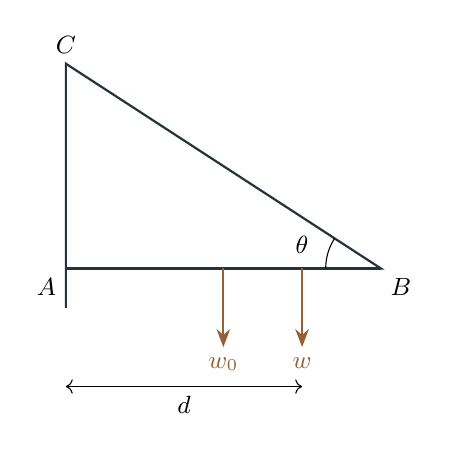
\begin{tikzpicture}
\coordinate(A)at(0,0);\coordinate(B)at(4,0);\coordinate(C)at(0,2.6);\draw[object] (0,-.5)--(C)--(B)--(A);\draw[object] (A)--(B);\draw (3.3,0) arc(180:147:.7);\node at (3.0,.3){$\theta$};\foreach \p/\pos in {A/below left,B/below right,C/above}{\node[\pos]at(\p){$\p$};}\draw[force] (2,0)--(2,-1)node[below]{$w_0$};\draw[force] (3,0)--(3,-1)node[below]{$w$};\draw[<->] (0,-1.5)--(3,-1.5)node[midway,below]{$d$};
\end{tikzpicture}
\figcaption{图 5.2\quad 杆端 $A$ 接触墙，$B$ 端用绳悬于 $C$，挂点距 $A$ 为 $d$。}
\end{minipage}\end{center}

\Needspace{5\baselineskip}

\pdfbookmark[3]{题型定位}{q2-h0}

\subsection*{题型定位}

刚体平衡、静摩擦下限与载荷位置的联合问题。杆受墙、绳、自重和附加重物作用，合力与力矩条件共同确定所需摩擦和墙压。

第一问确定基准状态，第二问把悬点位置变成变量。两问都先求实际静摩擦，再与最大值比较；载荷移动同时改变两者的比值，需要保留两个中间力。

\Needspace{5\baselineskip}

\pdfbookmark[3]{知识点}{q2-h1}

\subsection*{知识点}

\begin{itemize}
\tightlist
\item
  刚体三方程平衡
\item
  墙面支持力与静摩擦力
\item
  绳张力分解
\item
  对端点取矩消元
\item
  附加重物位置对摩擦下限的影响
\end{itemize}

杆的静力平衡同时需要合力为零与合力矩为零，选墙接触点取矩可消去墙的支持力和摩擦。求出绳张力后，再由竖直平衡求实际墙摩擦；与最大静摩擦力比较即可判断是否静止。载荷位置改变力矩，同时改变墙摩擦与法向力的比值。


\Needspace{5\baselineskip}

\pdfbookmark[3]{物理图像}{q2-h2}

\subsection*{物理图像}

解图5.2A中，墙给 $A$ 端水平向右的压力和向上的摩擦，绳在 $B$ 端向左上方拉。重物靠近 $A$ 时，对 $B$ 的力矩更大，需要更大的墙端摩擦；同时绳的竖直分量较小，墙压也较小。

应分别说明力矩转向：关于 $B$，向上的墙端摩擦产生顺时针力矩，两个重力产生逆时针力矩。关于 $A$ 则绳的竖直分量与重力相抵。两种取矩都可用，直接求 $f$ 时取 $B$ 更方便。

\Needspace{5\baselineskip}

\pdfbookmark[3]{解题入口}{q2-h3}

\subsection*{解题入口}

先对 $B$ 取矩，得到 $fl=w_0l/2+w(l-d)$，再求 $T\sin\theta=w_0+w-f$ 和 $N=T\cos\theta$。最后比较 $f/N$ 与 $\mu$。

不挂重物时取 $w=0$，挂半杆重时取 $w=w_0/2$。对 $A$ 取矩，墙端压力与摩擦的力矩均为零，可直接求绳张力。对 $B$ 取矩，绳张力与沿杆的墙压均无力矩，墙摩擦的力矩平衡两个重力矩。两个结果相加，给出竖直平衡式。

\Needspace{5\baselineskip}

\pdfbookmark[3]{标准解法}{q2-h4}

\subsection*{标准解法}

\textbf{墙面摩擦与杆的平衡。}解图5.2A中，墙对杆的法向力 $N$ 水平向右，摩擦力 $f$ 竖直向上，绳张力 $T$ 沿 $BC$ 指向 $C$。静摩擦条件是 $f\le\mu N$，只有临界状态才取等号。
\begin{center}\begin{minipage}{\linewidth}\centering
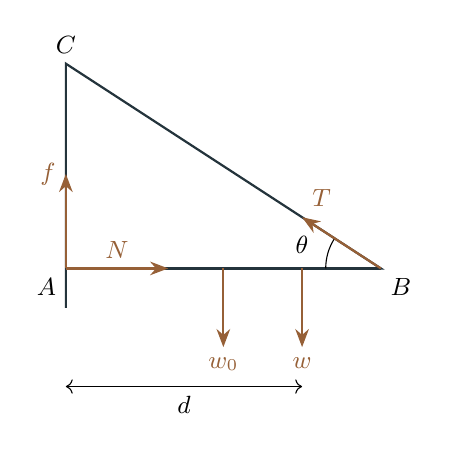
\begin{tikzpicture}
\coordinate(A)at(0,0);\coordinate(B)at(4,0);\coordinate(C)at(0,2.6);\draw[object] (0,-.5)--(C)--(B)--(A);\draw[object] (A)--(B);\draw (3.3,0) arc(180:147:.7);\node at (3.0,.3){$\theta$};\foreach \p/\pos in {A/below left,B/below right,C/above}{\node[\pos]at(\p){$\p$};}\draw[force] (2,0)--(2,-1)node[below]{$w_0$};\draw[force] (3,0)--(3,-1)node[below]{$w$};\draw[<->] (0,-1.5)--(3,-1.5)node[midway,below]{$d$};\draw[force] (0,0)--(0,1.2)node[left]{$f$};\draw[force] (0,0)--(1.3,0)node[midway,above]{$N$};\draw[force] (4,0)--(3, .65)node[above right]{$T$};
\end{tikzpicture}
\figcaption{解图 5.2A\quad 选 $B$ 为力矩中心可消去绳张力；重物在杆内时，墙上摩擦向上。}
\end{minipage}\end{center}
水平、竖直平衡分别为
\begin{align*}
 N&=T\cos\theta,\\
 f+T\sin\theta&=w_0+w.
\end{align*}
对 $B$ 取矩，绳张力的力矩为零。$N$ 的作用线沿杆，也没有力矩。摩擦力与两个重力的力矩相抵：
\[
 fl=\frac{w_0l}{2}+w(l-d).
\]
因而
\[
 f=\frac{w_0}{2}+w\left(1-\frac dl\right),
 \qquad T\sin\theta=\frac{w_0}{2}+\frac{wd}{l},
 \qquad N=\left(\frac{w_0}{2}+\frac{wd}{l}\right)\cot\theta.
\]
当 $0\le d\le l$、$w\ge0$ 时，$f>0,N>0$，与图中的方向一致。

\textbf{第一问：不挂附加重物。}令 $w=0$，则 $f=w_0/2$，$N=(w_0/2)\cot\theta$，故
\[
 \boxed{\mu\ge\tan\theta}.
\]
所需摩擦力由平衡方程给出，在最小系数处恰达到最大静摩擦力 $f=\mu N$。

\textbf{第二问：附加重物为杆重的一半。}令 $w=w_0/2$，得到
\[
 f=\frac{w_0}{2}\left(2-\frac dl\right),
 \qquad N=\frac{w_0}{2}\left(1+\frac dl\right)\cot\theta.
\]
于是
\[
 \boxed{\mu_{\min}(d)=\frac{2l-d}{l+d}\tan\theta},
 \qquad 0\le d\le l.
\]
其导数为
\[
 \frac{\dd\mu_{\min}}{\dd d}
 =-\frac{3l\tan\theta}{(l+d)^2}<0.
\]
把重物从 $A$ 移向 $B$，所需摩擦力减小而法向力增大，所以所需摩擦系数单调减小。三个位置为
\[
 d=0:\ 2\tan\theta;\qquad
 d=l/2:\ \tan\theta;\qquad
 d=l:\ \tfrac12\tan\theta.
\]
给定墙面材料的$\mu$后，还可直接从结果读允许的挂重位置。记$c=\mu/\tan\theta$，静止条件为
\[c\ge\frac{2-d/l}{1+d/l}
\quad\Longrightarrow\quad \frac dl\ge\frac{2-c}{1+c}.\]
若 $c<1/2$，杆上没有可用挂点。若 $1/2\le c<2$，从 $d=l(2-c)/(1+c)$ 到右端点 $B$ 都可挂重物。若 $c\ge2$，整段 $0\le d\le l$ 都允许。解图5.2A中把重物向绳连接端移动，同时减小墙所需向上摩擦、增加绳张力的水平压紧分量，所以这两个作用共同降低摩擦系数要求。

对$A$取矩时，墙端两力作用于矩心，力矩为零。方程$Tl\sin\theta=w_0l/2+wd$先给出$T$，再由竖直平衡得到相同的$f$。
\subsubsection*{用图读挂点范围与摩擦余量}
令$x=d/l$、$c=\mu/\tan\theta$，解图5.2B画出所需系数
$c_{\min}(x)=(2-x)/(1+x)$。给定材料时$c$是水平线；
曲线给出各挂点所需的最小系数。给定挂点 $x$，材料线在该点的纵坐标满足 $c\ge c_{\min}(x)$ 时，杆能保持静止。
\begin{center}\begin{minipage}{\linewidth}\centering
\begin{tikzpicture}[x=5cm,y=1.6cm]
\draw[axis](0,0)--(1.18,0)node[right]{$x=d/l$};
\draw[axis](0,0)--(0,2.35)node[above]{$c=\mu/\tan\theta$};
\fill[accent!12](2/3,.8)--(1,.8)--(1,.5)
plot[domain=1:2/3,samples=40](\x,{(2-\x)/(1+\x)})--cycle;
\draw[traj,domain=0:1,samples=90]plot(\x,{(2-\x)/(1+\x)});
\draw[warm](0,.8)--(1.05,.8)node[right]{$c=0.8$};
\draw[guide](2/3,0)--(2/3,.8);
\foreach \x/\y/\lab in {0/2/{2},.5/1/{1},1/.5/{1/2}}
{\fill(\x,\y)circle(1.6pt);\node[above right]at(\x,\y){$\lab$};}
\node[below]at(.5,0){$1/2$};\node[below]at(2/3,0){$2/3$};\node[below]at(1,0){$1$};
\draw[<->,accent](2/3,.18)--(1,.18)node[midway,above]{允许挂点};
\end{tikzpicture}
\figcaption{解图5.2B\quad 材料示例$\mu=0.8\tan\theta$；阴影是供给上限与所需系数之差，须有$d/l\geq2/3$。}
\end{minipage}\end{center}
图中$x=1/2$给$c_{\min}=1$。
附加重物挂在杆中点时，它与杆重有同一作用线，
两者合起来相当于重量增大而作用点不动；
所需$f,N$都成为无附加重物时的$3/2$倍，所以比值仍是$\tan\theta$。


\subsubsection*{附加重量越大，摩擦条件一定越苛刻吗}
保留任意$w\geq0$，两平衡力给
\[
\mu_{\min}(x,w)
=\frac{w_0/2+w(1-x)}{w_0/2+wx}\tan\theta.
\]
固定挂点$x$，对$w$求导：
\[
\frac{\partial\mu_{\min}}{\partial w}
=\frac{(w_0/2)(1-2x)}{(w_0/2+wx)^2}\tan\theta.
\]
因此挂点在左半杆时，加重使所需系数增大；
在右半杆时，加重反而使所需系数减小；
恰在中点时系数与$w$无关。
挂点在右半杆时，增加重物使墙压增大得比所需摩擦快，因而比值下降。挂在最右端时，摩擦大小保持不变，墙压仍随重物增加。
这一区分需要同时保留$f$与$N$，只比较总重量或一个力矩看不出结果。

摩擦系数的下限由 $f/N$ 决定。绳和墙各自的负荷仍要由张力 $T$ 和墙压 $N$ 表示，绳张力为
\[
T=\frac{w_0/2+wx}{\sin\theta}.
\]
当$\theta$变小时，所需摩擦系数随$\tan\theta$减小，
但$T$及墙压$N=T\cos\theta$反而增大。
减小绳角会使防滑更容易，同时增大绳和墙承担的力。


\Needspace{5\baselineskip}

\pdfbookmark[3]{关键洞察}{q2-h5}

\subsection*{关键洞察}

静摩擦的大小由平衡所需决定，摩擦系数只是供给上限。重物位置改变了 $f$ 和 $N$ 两个量，单看一个力矩会遗漏墙压变化。

对 $B$ 取矩可直接得到摩擦，对 $A$ 取矩可直接得到绳的竖直分量。学生若能把两式与竖直平衡对应起来，就能解释为何重物移动到中点时仍得到第一问的 $\tan\theta$。

\Needspace{5\baselineskip}

\pdfbookmark[3]{易错点}{q2-h6}

\subsection*{易错点}

\begin{itemize}\item 静摩擦先按平衡求$f$，在临界状态取$f=\mu N$。\item 对 $B$ 取矩时，重物力臂为 $l-d$；对 $A$ 时才是 $d$。\item 对$A$取矩，墙的压力和摩擦均过矩心，力矩都为零。\item 墙压等于绳的水平分量，由水平平衡给出。\item 关于选定矩心，逐力标出转向；求得的$f,N$均为正，与图中的方向一致。\end{itemize}

\Needspace{5\baselineskip}

\pdfbookmark[3]{课堂讲解建议}{q2-h7}

\subsection*{课堂讲解建议}

先做不挂重物的一问，用 $B$ 点矩直接得到 $f=w_0/2$。再在解图5.2A挂上重物，让学生只修改其关于 $B$ 的力矩项，同时保留竖直方程求墙压。要求每一步都把实际静摩擦与供给上限分开写。

将重物分别放在 $d=0,l/2,l$，请学生算出所需摩擦系数 $2\tan\theta,\tan\theta,\tan\theta/2$。再问“重物向右移动时，墙面摩擦和墙压各怎样变？”摩擦减少，墙压增大。若改对 $A$ 取矩，墙端两力的力矩都为零，直接得到 $Tl\sin\theta=w_0l/2+wd$。

在解图5.2B 取 $c=0.8$，由交点读出 $d/l\geq2/3$，再由摩擦不等式求同一个范围。问“加重时摩擦系数下限怎样变？”由 $\partial\mu_{\min}/\partial w$ 的符号区分左右半杆。对于系数下降的分支，请学生同时写出绳张力和墙压随重物变化的关系。

\Needspace{5\baselineskip}

\pdfbookmark[3]{变式训练}{q2-h8}

\subsection*{变式训练}

\begin{enumerate}
\item 减小绳与水平杆的夹角，求摩擦系数变化。令$x=d/l$，变图5.2V1 在$B$端分解绳力，$S=T\sin\theta=w_0/2+wx$由力矩决定，与$\theta$无关。水平平衡给$N=S\cot\theta$，摩擦仍为$f=w_0/2+w(1-x)$，故$\mu_{\min}=(f/S)\tan\theta$。减小$\theta$使$N$增大，而$f$保持原值；同时$T=S/\sin\theta$增大。
\begin{center}\begin{minipage}{.98\linewidth}\centering
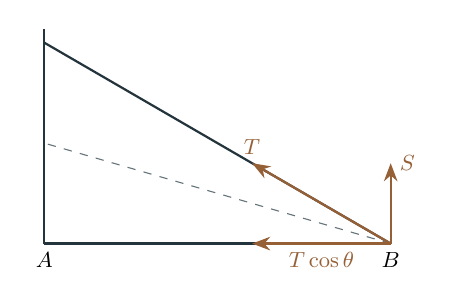
\begin{tikzpicture}[scale=.88,transform shape]
\draw[object] (0,0)--(5,0);\draw[object] (0,0)--(0,3.1);
\draw[object] (5,0)--(0,2.9);\draw[guide] (5,0)--(0,1.45);
\draw[force] (5,0)--(3,1.16) node[above] {$T$};
\draw[force] (5,0)--(5,1.16) node[right] {$S$};
\draw[force] (5,0)--(3,0) node[midway,below] {$T\cos\theta$};
\node[below] at (0,0) {$A$};\node[below] at (5,0) {$B$};
\end{tikzpicture}
\figcaption{变图5.2V1\quad 固定竖直分量时，减小绳角会增加水平分量。}
\end{minipage}\end{center}
\item 半杆重挂在$B$端。对$B$取矩，附加重物的力臂为零，故$fl=w_0l/2$，$f=w_0/2$。竖直平衡给$T\sin\theta=w_0$，所以$N=w_0\cot\theta$，$\mu_{\min}=\tan\theta/2$。变图5.2V2 中杆中点的自重仍需墙端摩擦提供力矩，$B$端重物增加绳力的竖直、水平分量。
\begin{center}\begin{minipage}{.98\linewidth}\centering
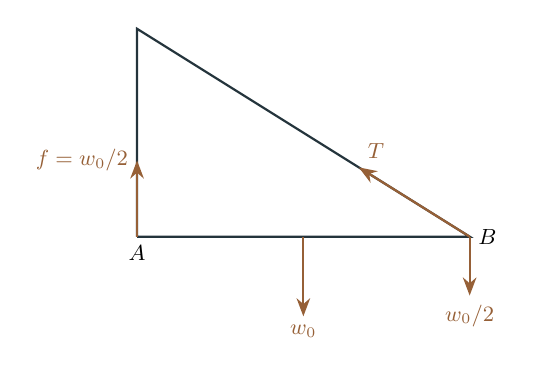
\begin{tikzpicture}[scale=.88,transform shape]
\draw[object] (0,0)--(4.8,0)--(0,3)--(0,0);
\draw[force] (0,0)--(0,1.1) node[left] {$f=w_0/2$};
\draw[force] (2.4,0)--(2.4,-1.15) node[below] {$w_0$};
\draw[force] (4.8,0)--(4.8,-.85) node[below] {$w_0/2$};
\draw[force] (4.8,0)--(3.2,1) node[above right] {$T$};
\node[below] at (0,0) {$A$};\node[right] at (4.8,0) {$B$};
\end{tikzpicture}
\figcaption{变图5.2V2\quad 附加重物在绳端，对该端的力矩为零。}
\end{minipage}\end{center}
\item 墙面光滑时，$A$端仅有水平支持力。变图5.2V3 对$B$取矩，水平支持力沿杆，绳力经过$B$，都无力矩。两个重力给出同向力矩$w_0l/2+w(l-d)>0$，在$w_0>0,\ w\ge0,\ 0\le d\le l$时始终为正，因此这一水平杆构型没有静止解。
\begin{center}\begin{minipage}{.98\linewidth}\centering
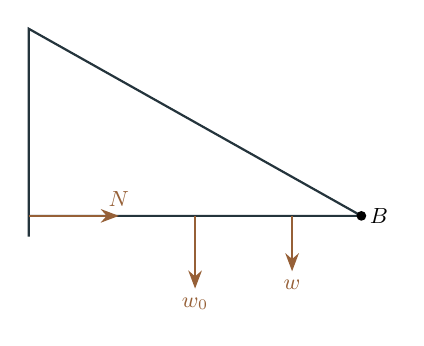
\begin{tikzpicture}[scale=.88,transform shape]
\draw[object] (0,-.3)--(0,2.7)--(4.8,0)--(0,0);
\draw[force] (0,0)--(1.3,0) node[above] {$N$};
\draw[force] (2.4,0)--(2.4,-1.05) node[below] {$w_0$};
\draw[force] (3.8,0)--(3.8,-.8) node[below] {$w$};
\fill (4.8,0) circle(2pt) node[right] {$B$};
\end{tikzpicture}
\figcaption{变图5.2V3\quad 光滑墙没有提供反向力矩的竖直作用。}
\end{minipage}\end{center}
\item 绳接在杆中点$C$，仍与杆成$\theta$。变图5.2V4 对$A$取矩，$T\sin\theta\,(l/2)=w_0l/2+wd$。于是
\[
T\sin\theta=w_0+2wx,\quad f=w(1-2x),\quad N=(w_0+2wx)\cot\theta .
\]
所需系数为$|f|/N$。$x<1/2$时摩擦向上，$x>1/2$时向下；无附加重物时$f=0$。变图5.2V4 在$C$的竖直力矩使两个方向均可直接由平衡式读出。
\begin{center}\begin{minipage}{.98\linewidth}\centering
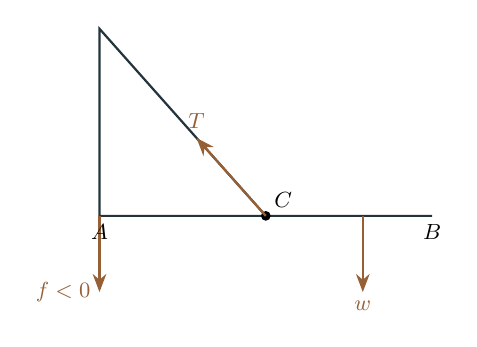
\begin{tikzpicture}[scale=.88,transform shape]
\draw[object] (0,-.3)--(0,2.7)--(2.4,0)--(0,0)--(4.8,0);
\fill (2.4,0) circle(2pt) node[above right] {$C$};
\draw[force] (2.4,0)--(1.4,1.125) node[above] {$T$};
\draw[force] (3.8,0)--(3.8,-1.1) node[below] {$w$};
\draw[force] (0,0)--(0,-1.1) node[left] {$f<0$};
\node[below] at (0,0) {$A$};\node[below] at (4.8,0) {$B$};
\end{tikzpicture}
\figcaption{变图5.2V4\quad 例取重物在右半杆，墙端摩擦改为向下。}
\end{minipage}\end{center}
\item 将半杆重缓慢从$A$移到$B$。令$c_{\min}=\mu_{\min}/\tan\theta=(2-x)/(1+x)$，求导得$c_{\min}'=-3/(1+x)^2<0$、$c_{\min}''=6/(1+x)^3>0$。变图5.2V5 连接$(0,2),(1/2,1),(1,1/2)$，曲线下降且向上凸。每一位置的$f,N$分别由静力平衡确定，沿准静态移动可依次使用这些结果。
\begin{center}\begin{minipage}{.98\linewidth}\centering
\begin{tikzpicture}[scale=.88,transform shape]
\draw[axis] (0,0)--(6.5,0) node[right] {$x=d/l$};
\draw[axis] (0,0)--(0,3.4) node[above] {$c_{\min}$};
\draw[traj,domain=0:1,samples=80] plot({5.5*\x},{1.5*(2-\x)/(1+\x)});
\foreach \xx/\yy/\ll in {0/3/2,2.75/1.5/1,5.5/.75/{1/2}}{\fill(\xx,\yy)circle(1.6pt);\node[above right] at(\xx,\yy){$\ll$};}
\end{tikzpicture}
\figcaption{变图5.2V5\quad 需求系数随挂点右移而下降，下降速率也逐渐减小。}
\end{minipage}\end{center}
\item 比较三个取矩点。变图5.2V6 把$A,C,B$标在同一杆上，$C$是中点。以逆时针为正，对$A$得$Tl\sin\theta=w_0l/2+wd$；对$B$得$fl=w_0l/2+w(l-d)$。对$C$，杆重过矩心，绳竖直力和墙摩擦的力臂均为$l/2$，得到
\[
(T\sin\theta-f)\frac l2=w(d-l/2).
\]
挂点在 $C$ 左侧时 $d<l/2$，右侧时 $d>l/2$，右端分别取负值和正值。前两式相加给竖直平衡，前两式相减给第三式。
\begin{center}\begin{minipage}{.98\linewidth}\centering
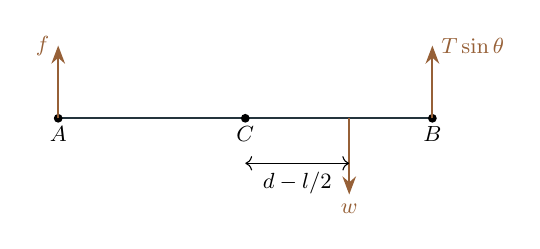
\begin{tikzpicture}[scale=.88,transform shape]
\draw[object] (0,0)--(5.4,0);
\foreach \xx/\ll in {0/A,2.7/C,5.4/B}{\fill(\xx,0)circle(1.8pt);\node[below]at(\xx,0){$\ll$};}
\draw[force] (0,0)--(0,1.05) node[left] {$f$};
\draw[force] (5.4,0)--(5.4,1.05) node[right] {$T\sin\theta$};
\draw[force] (4.2,0)--(4.2,-1.1) node[below] {$w$};
\draw[<->] (2.7,-.65)--(4.2,-.65) node[midway,below] {$d-l/2$};
\end{tikzpicture}
\figcaption{变图5.2V6\quad 不同矩心消去不同的力，重物对中点的力臂保留符号。}
\end{minipage}\end{center}\end{enumerate}

\clearpage

\pdfbookmark[2]{第 3 题 竖杆受水平力的防滑条件}{q3}

\section*{第 3 题\quad 竖杆受水平力的防滑条件}

\tagline{M-05-03}

质量为 $m$、长为 $L$ 的均匀细杆竖直放置，下端接触水平地面，静摩擦系数为 $\mu$。上端由轻绳拉住，绳的另一端固定在左下方，绳与竖杆的夹角为 $\theta$，$0<\theta<\pi/2$。在离地高度 $h$ 处向右施加水平力 $F$，$0\le h\le L$。求保持杆不滑倒所允许的 $F$ 的最大值，并讨论何时仅凭摩擦条件不能给出有限上限。

\begin{center}\begin{minipage}{\linewidth}\centering
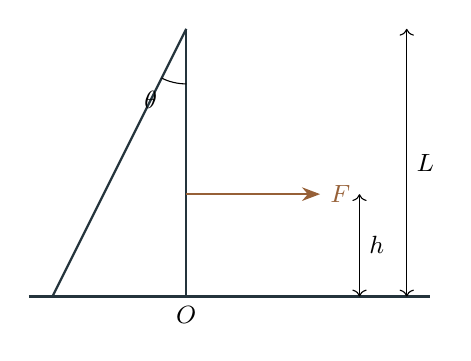
\begin{tikzpicture}
\draw[object](-2,0)--(3.1,0);
\draw[object](0,0)--(0,3.4);\draw[object](-1.7,0)--(0,3.4);
\draw(0,2.7)arc(-90:-116.565051177:.7);\node at(-.45,2.5){$\theta$};
\draw[force](0,1.3)--(1.7,1.3)node[right]{$F$};
\draw[<->](2.2,0)--(2.2,1.3)node[midway,right]{$h$};
\draw[<->](2.8,0)--(2.8,3.4)node[midway,right]{$L$};
\node[below]at(0,0){$O$};
\end{tikzpicture}
\figcaption{图5.3\quad 绳固定在左下方，推力高度$h$与杆长$L$分别标出。}\end{minipage}\end{center}

\Needspace{5\baselineskip}

\pdfbookmark[3]{题型定位}{q3-h0}

\subsection*{题型定位}

斜绳约束下竖杆的防滑条件。推力和作用高度决定绳张力，绳又改变地面压力，所以摩擦需求与摩擦能力都随推力增长。

本题除了三条平衡方程，还要处理不等式系数的正、零、负三类。有限上限与理想模型无有限上限属于不同参数区，应连同作用高度的趋势一起讲清。

\Needspace{5\baselineskip}

\pdfbookmark[3]{知识点}{q3-h1}

\subsection*{知识点}

\begin{itemize}
\tightlist
\item
  竖直杆刚体平衡
\item
  地面静摩擦临界
\item
  绳张力分解
\item
  对杆下端取矩
\item
  外力作用高度的力臂效应
\end{itemize}

水平外力、绳拉力与地面摩擦共同平衡，受力高度决定各自分担比例。先用力矩消去不需要的力，再将实际静摩擦与$\mu N$比较。作用点到杆顶的退化情形可令所需摩擦为零，除以该距离之前须单独保留。


\Needspace{5\baselineskip}

\pdfbookmark[3]{物理图像}{q3-h2}

\subsection*{物理图像}

绳固定在杆上端的左下方，因此张力向左下。地面摩擦向左抵抗推力，地面支持力还要承受绳的向下分量。解图5.3A把 $h$ 和 $L$ 分开标注，推力、绳水平分量的力臂分别是这两个长度。

增加 $h$ 会增加为抵消推力矩所需的绳张力，却减少地面需要承担的水平摩擦。地面所需摩擦为$f=(1-h/L)F$，支持力为$N=mg+(Fh/L)\cot\theta$；比较两者之比与$\mu$，便得到作用高度对防滑条件的影响。

\Needspace{5\baselineskip}

\pdfbookmark[3]{解题入口}{q3-h3}

\subsection*{解题入口}

对底端取矩求 $T\sin\theta=Fh/L$，随后求 $f$ 和 $N$。先写 $[L-h-\mu h\cot\theta]F\le\mu mgL$，再分类讨论系数的符号。

系数正时有有限上限，非正时摩擦条件对任意非负推力成立。有限强度绳若另有 $T_{\max}$，还须叠加张力限制。将未经除法的不等式保留在板书上，便于处理 $h=0,L$ 和 $\mu=0$。

\Needspace{5\baselineskip}

\pdfbookmark[3]{标准解法}{q3-h4}

\subsection*{标准解法}

\textbf{力的方向。}解图5.3A中，绳张力的水平分量向左、竖直分量向下；地面摩擦 $f$ 向左，支持力 $N$ 向上。由于杆保持竖直，重力通过下端 $O$，对 $O$ 不产生力矩。
\begin{center}\begin{minipage}{\linewidth}\centering
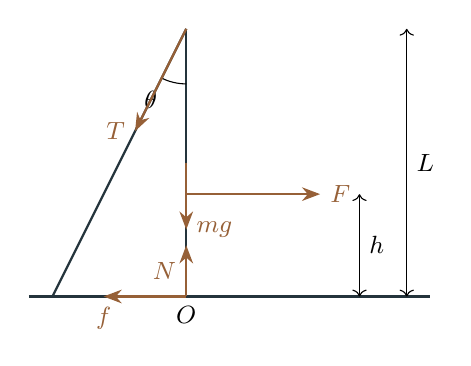
\begin{tikzpicture}
\draw[object](-2,0)--(3.1,0);
\draw[object](0,0)--(0,3.4);\draw[object](-1.7,0)--(0,3.4);
\draw(0,2.7)arc(-90:-116.565051177:.7);\node at(-.45,2.5){$\theta$};
\draw[force](0,1.3)--(1.7,1.3)node[right]{$F$};
\draw[<->](2.2,0)--(2.2,1.3)node[midway,right]{$h$};
\draw[<->](2.8,0)--(2.8,3.4)node[midway,right]{$L$};
\node[below]at(0,0){$O$};
\draw[force](0,3.4)--(-.65,2.1)node[left]{$T$};
\draw[force](0,0)--(-1.05,0)node[below]{$f$};
\draw[force](0,0)--(0,.65)node[midway,left]{$N$};
\draw[force](0,1.7)--(0,.85)node[right]{$mg$};
\end{tikzpicture}
\figcaption{解图5.3A\quad 地面摩擦向左，绳向下压紧；箭头标各力实际作用点和方向，大小由平衡方程确定。}\end{minipage}\end{center}
对 $O$ 取矩，并列水平、竖直平衡：
\begin{align*}
 TL\sin\theta&=Fh,\\
 T\sin\theta+f&=F,\\
 N&=mg+T\cos\theta.
\end{align*}
故
\[
 T=\frac{Fh}{L\sin\theta},\qquad
 f=F\left(1-\frac hL\right),\qquad
 N=mg+\frac{Fh}{L}\cot\theta.
\]
$0\le h\le L$ 时 $f\ge0$，所假定的向左方向成立。若改对杆上端取矩，直接得到 $fL=F(L-h)$，也得到相同的摩擦力。

\textbf{地面摩擦与推力范围。}不滑动要求
\[
 F\left(1-\frac hL\right)
 \le\mu\left(mg+\frac{Fh}{L}\cot\theta\right),
\]
即
\[
 DF\le\mu mgL,\qquad
 D=L-h-\mu h\cot\theta.
\]
\begin{enumerate}
\item 若 $D>0$，才可除以 $D$ 而不改变不等号方向，得到有限上限
\[
 \boxed{F_{\max}=\frac{\mu mgL}{L-h-\mu h\cot\theta}
 =\frac{\mu mgL\tan\theta}{(L-h)\tan\theta-\mu h}}.
\]
此时 $h<L\tan\theta/(\mu+\tan\theta)$。
\item 若 $D\le0$，左端对任意 $F\ge0$ 均不为正，而右端不为负，摩擦条件始终满足。在理想刚杆、无限强度绳的模型中，$F$ 没有有限上限。绳的强度若有给定上限，再用张力式与该上限联立。
\end{enumerate}
\begin{center}\begin{minipage}{\linewidth}\centering
\begin{tikzpicture}[x=5.5cm,y=.9cm]
\fill[accent!8](.5,0)rectangle(1,4.35);
\draw[axis](0,0)--(1.14,0)node[right]{$h/L$};
\draw[axis](0,0)--(0,4.8)node[above]{$F_{\max}/mg$};
\draw[guide](.5,0)--(.5,4.4);
\draw[traj,domain=0:.44,samples=90]plot(\x,{.5/(1-2*\x)});
\foreach \x/\lab in {0/0,.25/{1/4},.5/{1/2},.75/{3/4},1/1}
{\draw(\x,-.06)--(\x,.06);\node[below]at(\x,-.1){$\lab$};}
\foreach \y in {1,2,3,4}{\draw(-.01,\y)--(.01,\y);\node[left]at(-.01,\y){$\y$};}
\node[left]at(0,.5){$\mu=1/2$};
\node[align=center]at(.77,2.7){摩擦条件\\不设有限上限};
\end{tikzpicture}
\figcaption{解图5.3B\quad 参数示例$\mu=1/2,\cot\theta=2$；$h/L<1/2$有有限上限，从 $h/L=1/2$ 起，摩擦条件对任意非负推力都成立。}
\end{minipage}\end{center}
\textbf{施力高度与两端情形。}解图5.3B中，在有限上限区，$D$ 随 $h$ 减小，因而 $F_{\max}$ 随 $h$ 增大。施力越高，绳承担的水平分力越多，地面所需摩擦越少；绳的向下分量同时增大 $N$。

$h=0$ 时绳不需张力，$F_{\max}=\mu mg$；$h=L$ 时 $f=0$，绳承担全部水平力，摩擦不限制 $F$。若 $\mu=0$，则除 $h=L$ 外只能有 $F=0$。这些结论也由未经除法的原始不等式直接得到。
\subsubsection*{从摩擦比的增长率解释无有限上限}
令$x=h/L$。在给定作用高度下，所需摩擦与地面支持力之比为
\[
\frac fN=\frac{(1-x)F}{mg+xF\cot\theta}.
\]
对$0\leq x<1$，它随$F$增加而增加：
\[
\frac{\partial(f/N)}{\partial F}
=\frac{(1-x)mg}{(mg+xF\cot\theta)^2}>0.
\]
$x=0$时这个比值没有上界，恢复$F\leq\mu mg$。
对$0<x<1$，其极限却是有限的
\[
\lim_{F\to\infty}\frac fN
=\frac{1-x}{x}\tan\theta.
\]
若材料的$\mu$不小于这个极限，就不会与增长中的$f/N$发生交叉，
所以理想静摩擦条件不能给有限最大推力。
将该条件整理，正是$x\geq\tan\theta/(\mu+\tan\theta)$。
当 $\mu>0$、$D=0$ 时，法向力仍含正的常量 $mg$，因而每个有限的 $F$ 都有 $f<\mu N$。只有在 $F\to\infty$ 的极限，所需的摩擦比才趋于 $\mu$。

有限上限区中还可直接求导：
\[
\frac{\dd F_{\max}}{\dd h}
=\frac{\mu mgL(1+\mu\cot\theta)}
{(L-h-\mu h\cot\theta)^2}>0\quad(\mu>0).
\]
解图5.3B采用$\mu=1/2,\cot\theta=2$的一组参数，
渐近线确在$h/L=1/2$，曲线为$F_{\max}/mg=(1/2)/(1-2h/L)$。
图中横坐标使用实际无量纲高度，渐近线右侧仍属于$0\leq h/L\leq1$的允许几何，
表示任意非负推力都满足静摩擦条件。

若固定$F>0$反求高度，未经除法的不等式给
\[
\frac hL\geq
\frac{1-\mu mg/F}{1+\mu\cot\theta}.
\]
当$F\leq\mu mg$，右端非正，任意高度均可；
当$F>\mu mg$，须把施力点提高到所给下界。
这一结论与$F_{\max}$随高度增大的曲线相符。


\Needspace{5\baselineskip}

\pdfbookmark[3]{关键洞察}{q3-h5}

\subsection*{关键洞察}

地面所需摩擦$f=(1-h/L)F$与可供上限$\mu N$都随推力增大，是否相交取决于增长率。$D\leq0$时摩擦约束不设有限上限；$\mu>0,D=0$时有限推力还未满摩擦，只有极限比值达到$\mu$。施力点升高时绳分担更多水平力，同时增加向下压紧分量，因此有限上限区允许更大的$F$。地面支持力由$N$给出；若给定绳强度，则把$T=Fh/(L\sin\theta)$与强度上限联立。

\Needspace{5\baselineskip}

\pdfbookmark[3]{易错点}{q3-h6}

\subsection*{易错点}

\begin{itemize}\item $\theta$ 相对竖杆测量，张力水平分量为 $T\sin\theta$。\item 有张力时绳向下压杆，$N>mg$；$T=0$ 时 $N=mg$。地面力对下端均无力矩。\item 绳的水平分量承担$Fh/L$，剩余的$F(1-h/L)$由地面摩擦承担。\item 当 $D>0$，摩擦条件给出推力上限。$D\le0$ 时摩擦条件对全部非负推力成立。\item 固定推力时，摩擦不等式给作用高度的下限，几何上端为$L$。\item 绳强度有限时，再按$T\le T_{\max}$计算允许推力，与摩擦范围相交。\end{itemize}

\Needspace{5\baselineskip}

\pdfbookmark[3]{课堂讲解建议}{q3-h7}

\subsection*{课堂讲解建议}

先在解图5.3A画推力的转动趋势，要求绳在上端提供反向力矩。地面摩擦的方向随后由水平平衡确定。板书分别框出 $f(F,h)$ 和 $N(F,h)$，让学生口述作用点升高时两者的变化。

写出 $DF\le\mu mgL$ 后，请学生分别取 $D>0,D=0,D<0$，说明哪一种情况给出有限推力上限。$D>0$ 时有有限上限。再把施力点移到 $h=L$，由水平平衡读出地面摩擦为零，全部水平推力由绳张力平衡。固定 $F$ 时，请学生解出允许的最低施力高度。

再画$f/N$随$F$增加的曲线，比较其极限$(1-h/L)L\tan\theta/h$与$\mu$。
要求解释$\mu>0,D=0$时有限推力为何仍未达到满摩擦：重力在支持力中留下一个正的常量项。
把解图5.3B的$\mu=1/2,\cot\theta=2$代入$D$，让学生算出渐近线$h/L=1/2$并标在横轴上。

\Needspace{5\baselineskip}

\pdfbookmark[3]{变式训练}{q3-h8}

\subsection*{变式训练}

\begin{enumerate}
\item 绳接在$H_s=L/2$处。变图5.3V1 对底端取矩，$T H_s\sin\theta=Fh$，再列水平、竖直平衡，得
\[
f=F(1-h/H_s),\qquad N=mg+(Fh/H_s)\cot\theta .
\]
这里$f$取向左为正，防滑条件是$|f|\le\mu N$。$h<H_s$时摩擦向左，$h>H_s$时绳的水平分量大于推力，摩擦改向右；$h=H_s$时恰为零。
\begin{center}\begin{minipage}{.98\linewidth}\centering
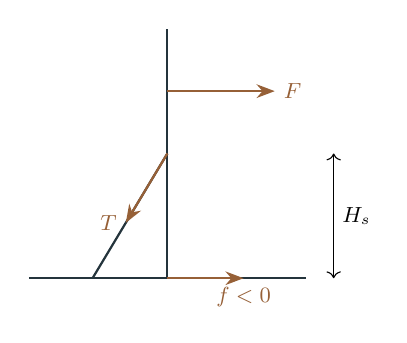
\begin{tikzpicture}[scale=.88,transform shape]
\draw[object](-2,0)--(2,0);\draw[object](0,0)--(0,3.6);
\draw[object](-1.08,0)--(0,1.8);
\draw[force](0,2.7)--(1.55,2.7)node[right]{$F$};
\draw[force](0,1.8)--(-.6,.8)node[left]{$T$};
\draw[force](0,0)--(1.1,0)node[below]{$f<0$};
\draw[<->](2.4,0)--(2.4,1.8)node[midway,right]{$H_s$};
\end{tikzpicture}
\figcaption{变图5.3V1\quad 例取施力点高于绳接点，地面摩擦向右。}
\end{minipage}\end{center}
\item 比较$h=0$和$h=L$。变图5.3V2 左图中，推力过底端，力矩平衡给$T=0$，于是$f=F,\ N=mg$，$F\le\mu mg$。右图中推力在顶端，$T\sin\theta=F$，水平力完全由绳抵消，$f=0$且$N=mg+F\cot\theta$。地面摩擦在后一情形不设有限推力上限。
\begin{center}\begin{minipage}{.98\linewidth}\centering
\begin{tikzpicture}[scale=.88,transform shape]
\foreach \xx/\lab in {0/0,4.4/L}{
\draw[object] (\xx-1.45,0)--++(3.45,0);
\draw[object] (\xx,0)--++(0,3.0);
\node[below] at (\xx,-.3) {$h=\lab$};}
\draw[force](0,0)--(1.5,0)node[above]{$F$};
\draw[force](0,0)--(-1.5,0)node[above]{$f$};
\draw[force](4.4,3)--(5.9,3)node[right]{$F$};
\draw[force](4.4,3)--(2.9,1.6)node[left]{$T$};
\end{tikzpicture}
\figcaption{变图5.3V2\quad 底端推力由摩擦承担，顶端推力由绳的水平分量承担。}
\end{minipage}\end{center}
\item 将推力反向，绳固定端仍在左下方。变图5.3V3 的两个水平向左分量都给底端逆时针力矩。若$h>0$，矩方程为$Fh+TL\sin\theta=0$，$F>0,T\ge0$时没有解。若把绳固定端同时移到右下方，受力图左右镜像，所有大小关系恢复。$h=0$时可取$T=0$，由向右摩擦抵抗反向推力。
\begin{center}\begin{minipage}{.98\linewidth}\centering
\begin{tikzpicture}[scale=.88,transform shape]
\draw[object](-2,0)--(2,0);\draw[object](0,0)--(0,3.4);
\draw[object](-1.41667,0)--(0,3.4);
\draw[force](0,1.9)--(-1.6,1.9)node[left]{$F$};
\draw[force](0,3.4)--(-.7,1.72)node[left]{$T$};
\fill(0,0)circle(2pt)node[below]{$O$};
\node[right] at (.45,2.5){两力矩同向};
\end{tikzpicture}
\figcaption{变图5.3V3\quad 绳的拉力保持非负时，反向推力与原绳的力矩同向。}
\end{minipage}\end{center}
\item 地面光滑时求非零推力的作用点。水平平衡要求$T\sin\theta=F$，底端矩要求$TL\sin\theta=Fh$，两式联立得$h=L$。变图5.3V4 中绳的水平分量抵消顶端推力，向下分量由地面承担，$N=mg+F\cot\theta$。任意$h<L$的非零推力均留下底端力矩。
\begin{center}\begin{minipage}{.98\linewidth}\centering
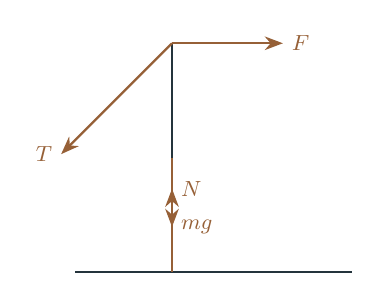
\begin{tikzpicture}[scale=.88,transform shape]
\draw[object](-1.4,0)--(2.6,0);\draw[object](0,0)--(0,3.3);
\draw[force](0,3.3)--(1.6,3.3)node[right]{$F$};
\draw[force](0,3.3)--(-1.6,1.7)node[left]{$T$};
\draw[force](0,0)--(0,1.2)node[right]{$N$};
\draw[force](0,1.65)--(0,.65)node[right]{$mg$};
\end{tikzpicture}
\figcaption{变图5.3V4\quad 光滑地面提供法向力，绳与推力在杆顶平衡水平分量。}
\end{minipage}\end{center}
\item 给定$F>0$求允许高度。将$F(1-h/L)\le\mu[mg+(Fh/L)\cot\theta]$展开，收集$h$项：
\[
h\ge\frac{L(1-\mu mg/F)}{1+\mu\cot\theta}.
\]
变图5.3V5 取$\mu=1/2,\cot\theta=2$，横轴为$s=F/(mg)$，曲线是$x_{\min}=\max(0,(1-\mu/s)/2)$。$s\le1/2$时整个$[0,L]$允许；更大的推力要求施力点提高到下限以上，上端仍为$L$。
\begin{center}\begin{minipage}{.98\linewidth}\centering
\begin{tikzpicture}[scale=.88,transform shape]
\draw[axis](0,0)--(6.9,0)node[right]{$s=F/(mg)$};
\draw[axis](0,0)--(0,3.35)node[above]{$h/L$};
\draw[guide](0,3)--(6.4,3)node[right]{$1$};
\draw[guide](0,1.5)--(6.4,1.5)node[right]{$1/2$};
\draw[traj](0,0)--(.75,0);
\draw[traj,domain=.5:4.2,samples=90]plot({1.5*\x},{1.5*(1-.5/\x)});
\node[below]at(.75,0){$1/2$};\node at(3.9,2.1){曲线上方允许};
\end{tikzpicture}
\figcaption{变图5.3V5\quad 固定推力所要求的是施力点下限。}
\end{minipage}\end{center}
\item 绳的最大张力为$T_{\max}$。变图5.3V6 中，$h>0$时由力矩式得$T=Fh/(L\sin\theta)$，因此
\[
F\le F_T(h)=T_{\max}L\sin\theta/h.
\]
同时保留摩擦约束$DF\le\mu mgL$。在$D>0$区，允许上限为$\min(F_{\max},F_T)$；在$D\le0$区，上限由$F_T$给出。$h=0$时绳不受力，允许$F\le\mu mg$。图中一条上升曲线与一条下降曲线相交，实际上限取两者较低部分。
\begin{center}\begin{minipage}{.98\linewidth}\centering
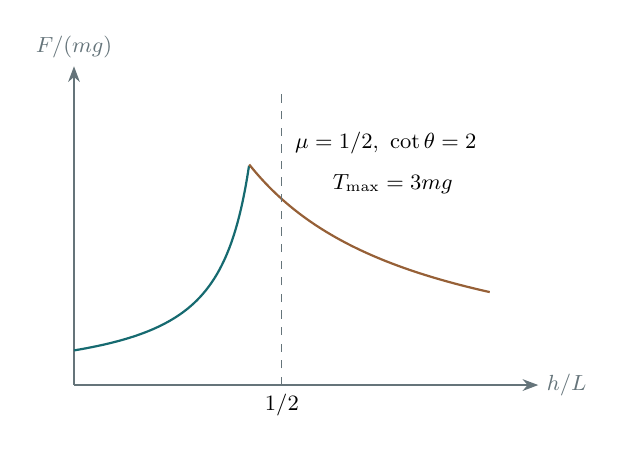
\begin{tikzpicture}[scale=.88,transform shape]
\pgfmathsetmacro{\crossHeight}{(3/sqrt(5))/(.5+6/sqrt(5))}
\draw[axis](0,0)--(6.7,0)node[right]{$h/L$};
\draw[axis](0,0)--(0,4.6)node[above]{$F/(mg)$};
\draw[traj,domain=0:\crossHeight,samples=90]plot({6*\x},{.5/(1-2*\x)});
\draw[object,thick,color=warm,domain=\crossHeight:1,samples=90]plot({6*\x},{3/(sqrt(5)*\x)});
\draw[guide](3,0)--(3,4.3);\node[below]at(3,0){$1/2$};
\node at(4.5,3.5){$\mu=1/2,\ \cot\theta=2$};
\node at(4.6,2.9){$T_{\max}=3mg$};
\end{tikzpicture}
\figcaption{变图5.3V6\quad 同时施加摩擦与绳强度限制，取下方的允许曲线。}
\end{minipage}\end{center}\end{enumerate}

\clearpage

\pdfbookmark[2]{第 4 题 半球凹面内的均匀细杆}{q4}

\section*{第 4 题\quad 半球凹面内的均匀细杆}

\tagline{M-05-04}

半径为 $R$ 的光滑半球形凹面内，一根刚性均匀细杆处于平衡。杆的一端接触内壁，杆身经过凹面边缘并伸出，如图所示。已知杆在凹面内的部分长为 $l$，求露出部分的长度，并给出该接触构型的适用范围。

\begin{center}\begin{minipage}{\linewidth}\centering
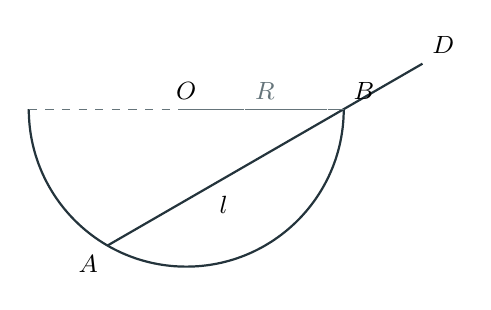
\begin{tikzpicture}
\coordinate(O)at(0,0);\coordinate(A)at(-1,-1.732050808);
\coordinate(B)at(2,0);\coordinate(D)at(3,.577350269);
\draw[object](-2,0)arc(180:360:2);\draw[guide](-2,0)--(2,0);
\draw[object](A)--(D);\draw[guide](O)--(B)node[midway,above]{$R$};
\node[above]at(O){$O$};\node[below left]at(A){$A$};
\node[above right]at(B){$B$};\node[above right]at(D){$D$};
\node[below right]at(.3,-.98){$l$};
\end{tikzpicture}
\figcaption{图5.4\quad 杆内端$A$接触凹面，杆身在边缘$B$处支承并伸出至$D$。}\end{minipage}\end{center}

\Needspace{5\baselineskip}

\pdfbookmark[3]{题型定位}{q4-h0}

\subsection*{题型定位}

非平行三力平衡与圆几何结合。光滑接触先给两条法线，三力共点确定整杆重心的竖直线，随后才由弦长、中点关系求露出长度。

取两支持力交点为矩心可同时消去它们的大小。力作用线的交点先确定整杆重心的竖直线，再由弦长求露出段。将露出长度与两法向力取非负，得到这一接触构型的长度范围。

\Needspace{5\baselineskip}

\pdfbookmark[3]{知识点}{q4-h1}

\subsection*{知识点}

\begin{itemize}
\tightlist
\item
  三力平衡共点条件
\item
  光滑接触面的法向反力
\item
  对交点取矩
\item
  圆内直角几何关系
\item
  均匀杆质心位置
\end{itemize}

光滑球面接触的支持力沿球半径，光滑口缘接触还受几何位置限制。三力平衡可用作用线共点或力矩方程，所得角度同时对应内壁与口缘两个接触点。代入两个支持力取非负，才能形成单侧接触的静止构型。


\Needspace{5\baselineskip}

\pdfbookmark[3]{物理图像}{q4-h2}

\subsection*{物理图像}

球面内端的支持力沿半径指向球心，边缘接触力垂直杆。延长这两条作用线得到 $E$，平衡要求整杆重心的铅垂线也通过 $E$。解图5.4A用辅助点$E$标出两力作用线的交点，实际接触点仍是$A,B$。

$AE$ 是截面圆的直径，$B$ 位于该圆上，因而 $BE\perp AB$。重心 $C$ 在杆内段靠近边缘的位置，但它是整根 $AD$ 的中点。解图5.4B将各段长度展开，有助于区分 $AB=l$、$AC=AD/2$ 和露出段 $BD$。

\Needspace{5\baselineskip}

\pdfbookmark[3]{解题入口}{q4-h3}

\subsection*{解题入口}

以两个法向力的交点 $E$ 为矩心，重力矩为零，推出 $EC$ 竖直。圆周角给出 $BE\perp AB$，勾股关系给出 $BE^2=4R^2-l^2$。

由两个三角形中同一个杆倾角推得 $CB=BE^2/l$，再用 $AC=CD$ 得到 $BD=l-2CB$。由$BD\ge0,l\le2R$和两支持力非负确定允许的内段长度，得到长度公式所对应的实际平衡范围。

\Needspace{5\baselineskip}

\pdfbookmark[3]{标准解法}{q4-h4}

\subsection*{标准解法}

\textbf{利用三力共点确定整杆重心。}设杆内端为 $A$，凹面边缘的接触点为 $B$，外端为 $D$，球心为 $O$，整杆重心为 $C$。光滑球面对 $A$ 的支持力沿 $AO$；边缘对细杆的支持力垂直杆。两条作用线交于 $E$。三个非平行力平衡，重力作用线也经过 $E$，因此 $EC$ 竖直。
\begin{center}\begin{minipage}{\linewidth}\centering
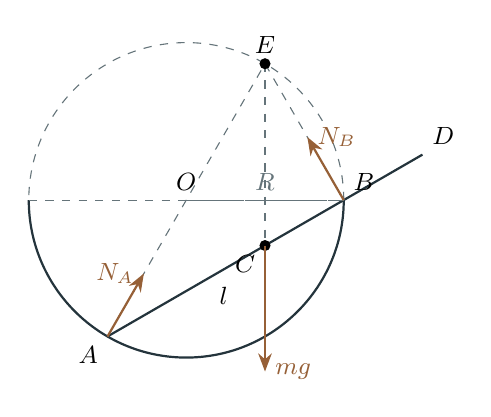
\begin{tikzpicture}
\coordinate(O)at(0,0);\coordinate(A)at(-1,-1.732050808);
\coordinate(B)at(2,0);\coordinate(D)at(3,.577350269);
\draw[object](-2,0)arc(180:360:2);\draw[guide](-2,0)--(2,0);
\draw[object](A)--(D);\draw[guide](O)--(B)node[midway,above]{$R$};
\node[above]at(O){$O$};\node[below left]at(A){$A$};
\node[above right]at(B){$B$};\node[above right]at(D){$D$};
\node[below right]at(.3,-.98){$l$};
\draw[guide](2,0)arc(0:180:2);
\coordinate(E)at(1,1.732050808);\coordinate(C)at(1,-.577350269);
\draw[guide](A)--(E)--(B);\draw[guide](E)--(C);
\fill(E)circle(2pt)node[above]{$E$};\fill(C)circle(2pt)node[below left]{$C$};
\draw[force](A)--(-.538119785,-.932050808)node[left]{$N_A$};
\draw[force](B)--(1.538119785,.8)node[right]{$N_B$};
\draw[force](C)--(1,-2.177350269)node[right]{$mg$};
\end{tikzpicture}
\figcaption{解图5.4A\quad 上半虚圆为辅助圆，$AE$为直径；$C$是整杆中点，三力作用线共点。}\end{minipage}\end{center}
在解图5.4A中，延长 $AO$ 到球面的另一交点 $E$。因 $AE$ 为直径、$B$ 在球面上，圆周角给出 $\angle ABE=90^\circ$，正好满足边缘法向力垂直杆。因此
\[
 AE=2R,\qquad AB=l,\qquad BE^2=4R^2-l^2.
\]
令杆与水平面的夹角为 $\gamma$。直角三角形 $ABE$ 中 $BE/l=\tan\gamma$，而 $EC$ 竖直，在三角形 $BCE$ 中 $CB/BE=\tan\gamma$。所以
\[
 CB=BE\tan\gamma=\frac{BE^2}{AB}
 =\frac{4R^2-l^2}{l}.
\]
\textbf{重心在整根杆的中点。}图中 $C$ 位于 $A,B$ 之间，$AC=l-CB$，均匀杆满足 $CD=AC$。于是露出长度
\begin{align*}
 BD&=CD-CB=AC-CB=l-2CB\\
 &=l-2\frac{4R^2-l^2}{l}
 =\boxed{\frac{3l^2-8R^2}{l}}.
\end{align*}
\begin{center}\begin{minipage}{\linewidth}\centering
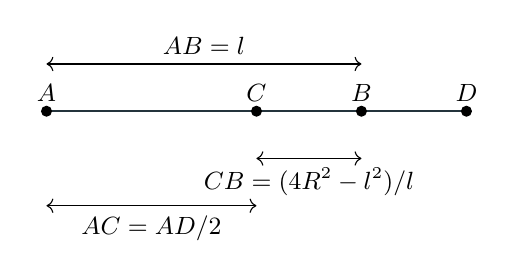
\begin{tikzpicture}
\coordinate(A)at(0,0);\coordinate(B)at(4,0);
\coordinate(D)at(5.333333333,0);\coordinate(C)at(2.666666667,0);
\draw[object](A)--(D);
\draw[<->](0,.6)--(4,.6)node[midway,above]{$AB=l$};
\draw[<->](2.666666667,-.6)--(4,-.6)node[midway,below]{$CB=(4R^2-l^2)/l$};
\draw[<->](0,-1.2)--(2.666666667,-1.2)node[midway,below]{$AC=AD/2$};
\foreach \p in {A,B,C,D}{\fill(\p)circle(2pt);\node[above]at(\p){$\p$};}
\end{tikzpicture}
\figcaption{解图5.4B\quad 与解图5.4A同一长度比例的展平图；$C$分的是整杆$AD$。}
\end{minipage}\end{center}
重力作用于整根杆$AD$的中点$C$。解图5.4B把$AC=AD/2$和$AB=l$分别标出。

\textbf{接触构型的范围。}弦长给出 $l\le2R$，且 $BD\ge0$ 要求
\[
 l\ge\sqrt{\frac83}\,R.
\]
若有实际露出部分并保持两个非退化接触，则
\[
 \boxed{\sqrt{8/3}\,R<l<2R}.
\]
长度取下限时 $BD=0$，外端恰在口缘。长度接近上限时，杆趋于水平，内端支持力趋于零。

几何关系 $l=2R\cos\gamma$ 给出 $0<\gamma\le35.264^\circ$。设整杆质量为 $m$，在这一角度范围内，将两个支持力分别沿水平和竖直方向投影，得到
\[
 N_A=mg\tan\gamma,\qquad
 N_B=mg\frac{\cos2\gamma}{\cos\gamma}.
\]
此范围两者均非负，故几何与单向接触条件一致。
\subsubsection*{由坐标求重心线和露出长度}
为明确两次倾角关系，在三角形$AOB$中$OA=OB=R$，
$\angle ABO=\gamma$，所以$\angle OAB=\gamma$；
$A,O,E$共线，故直角三角形$ABE$中的$\angle BAE$也为$\gamma$。
由直角三角形 $ABE$ 得 $BE/AB=\tan\gamma$。解图5.4A 的上半圆是延长后的辅助截面圆，$E$ 是两条支持力作用线的交点，实际接触点为 $A,B$。

也可令$B=(R,0)$，杆沿外伸方向的单位向量为
$\vect t=(\cos\gamma,\sin\gamma)$，整杆长为$s=AD$。
于是
\[
A=B-l\vect t,\qquad |OA|=R
\quad\Longrightarrow\quad l=2R\cos\gamma.
\]
支持力交点为$E=-A$，整杆中点$C=A+(s/2)\vect t$。
由重心线竖直，$C_x=E_x$：
\[
R-l\cos\gamma+\frac s2\cos\gamma
=-R+l\cos\gamma,
\]
\[
s=4l-\frac{4R}{\cos\gamma}
=4l-\frac{8R^2}{l},\qquad
BD=s-l=\frac{3l^2-8R^2}{l}.
\]
坐标式把弦长、整杆中点和三力共点连在一起。解图5.4A 中的 $C$ 与解图5.4B 的展开图对应，都是整个 $AD$ 的中点。两图取 $\gamma=30^\circ$、$l=2\sqrt3$、$R=2$，代入露出长度式得 $BD=2/\sqrt3$。

\subsubsection*{露出段消失和内端支持力消失}
在$A$，法向力方向与水平线夹角为$2\gamma$；
在$B$，法向力方向为$(-\sin\gamma,\cos\gamma)$。
水平和竖直分量方程为
\[
N_A\cos2\gamma-N_B\sin\gamma=0,\qquad
N_A\sin2\gamma+N_B\cos\gamma=mg.
\]
消元恢复$N_A=mg\tan\gamma$、$N_B=mg\cos2\gamma/\cos\gamma$，
因而不仅作用线共点，两支持力也都能以非负大小实现平衡。
在露出段刚为零的下界，$\cos\gamma=\sqrt{2/3}$，
\[
N_A=\frac{mg}{\sqrt2},\qquad N_B=\frac{mg}{\sqrt6},
\]
两者都没有消失，退化的是$BD$的长度。
在$l\to2R$的上界，$\gamma\to0$，才有$N_A\to0$、$N_B\to mg$；
此时$C$趋向边缘$B$，三力非平行的普通构型也随之退化。
下端先使露出段消失，上端则使内端支持力消失，分别对应上述两组极限。


\Needspace{5\baselineskip}

\pdfbookmark[3]{关键洞察}{q4-h5}

\subsection*{关键洞察}

光滑约束先给力的方向，三力共点再给重心的竖直线位置，无需求出接触力大小就能求杆长。这个方法适用于三个非平行外力，平行三力须另作取矩处理。

整杆中点与球内段中点不同，是长度计算的核心。露出构型取$BD\ge0$，这一条件给出$l$的下限；$l$降到下限时，外端$D$与口缘$B$重合。

\Needspace{5\baselineskip}

\pdfbookmark[3]{易错点}{q4-h6}

\subsection*{易错点}

\begin{itemize}\item 内壁支持力沿半径指向球心，口缘支持力沿杆的法线。\item $E$ 是两个支持力的交点，$AE$ 为直径的判断需要 $BE\perp AB$。\item $l$ 只指球内段，重心按整杆$AD$的质量分布确定。\item 由$BE/l=\tan\gamma$和$CB/BE=\tan\gamma$相乘，得到$CB=BE^2/l$。\item 长度范围由露出段非负、弦长不超过直径和法向力非负联立；上界内端法向力趋零。\end{itemize}

\Needspace{5\baselineskip}

\pdfbookmark[3]{课堂讲解建议}{q4-h7}

\subsection*{课堂讲解建议}

先复习非平行三力平衡的共点条件，再在解图5.4A延长两条法线找到 $E$。让学生指出为什么 $E$ 在截面圆上：$AE$ 是直径，圆周角使 $BE$ 垂直杆，与边缘支持力方向相符。

在解图5.4A 用两个直角三角形推出 $CB=BE^2/l$，再到解图5.4B 标出整杆中点。问“仅由两支支持力的方向，怎样确定重心线？”两支力的作用线交于 $E$，故重力作用线沿 $EC$。取 $l=R$，公式给出负的露出长度，该参数在所画构型之外。下端 $BD=0$ 时露出段缩为零，支持力仍为 $mg/\sqrt2$ 与 $mg/\sqrt6$。上端 $l\to2R$ 时，内端支持力 $N_A\to0$，边缘支持力 $N_B\to mg$。

\Needspace{5\baselineskip}

\pdfbookmark[3]{变式训练}{q4-h8}

\subsection*{变式训练}

\begin{enumerate}
\item 接触有摩擦时怎样求平衡构型？变图5.4V1 仍以$A$为内端、$B$为口缘。令杆单位方向$\boldsymbol t=(\cos\gamma,\sin\gamma)$，$A$处向内法线为$\boldsymbol n_A=(\cos2\gamma,\sin2\gamma)$，其切向取$\boldsymbol t_A=(-\sin2\gamma,\cos2\gamma)$；$B$处法线为$\boldsymbol n_B=(-\sin\gamma,\cos\gamma)$。总杆长为$s$时，对$A$取矩先得
\[
N_Bl=mg(s/2)\cos\gamma.
\]
再列$N_A\boldsymbol n_A+f_A\boldsymbol t_A+N_B\boldsymbol n_B+f_B\boldsymbol t-mg\boldsymbol e_y=0$，并取$N_A,N_B\ge0,\ |f_A|\le\mu_AN_A,\ |f_B|\le\mu_BN_B$。这组方程与不等式给出每个候选$l,s$是否可静止。此时两接触合力的交点随摩擦而变，三力共点仍成立，但交点由合力方向确定。
\begin{center}\begin{minipage}{.98\linewidth}\centering
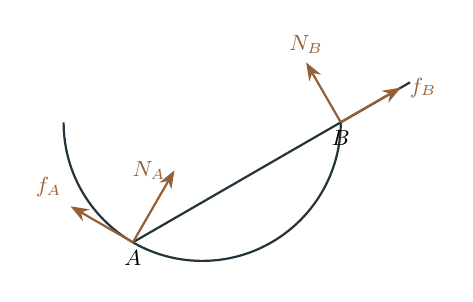
\begin{tikzpicture}[scale=.88,transform shape]
\coordinate(A)at(-1,-1.732); \coordinate(B)at(2,0);
\draw[object](-2,0)arc(180:360:2);\draw[object](A)--(3,.577);
\draw[force](A)--(-.4,-.693)node[left]{$N_A$};
\draw[force](A)--(-1.9,-1.212)node[above left]{$f_A$};
\draw[force](B)--(1.5,.866)node[above]{$N_B$};
\draw[force](B)--(2.866,.5)node[right]{$f_B$};
\node[below]at(A){$A$};\node[below]at(B){$B$};
\end{tikzpicture}
\figcaption{变图5.4V1\quad 摩擦使两接触合力偏离法线，分别在各自摩擦范围内取值。}
\end{minipage}\end{center}
\item 非均匀杆的重心距$A$为总杆长的$q$倍，$0<q<1$。变图5.4V2 中重力线仍通过两光滑法线的交点$E$，所以$AC=e=2l-4R^2/l$。由$AC=qAD$得
\[
AD=e/q,\qquad b=BD=\frac{2l-4R^2/l}{q}-l.
\]
要求$b\ge0$，等价于$l\ge2R/\sqrt{2-q}$；两接触保持非退化还取$l<2R$。该范围内$\gamma<45^\circ$，主解的两法向力为正。均匀时$q=1/2$给出$l\ge\sqrt{8/3}R$。
\begin{center}\begin{minipage}{.98\linewidth}\centering
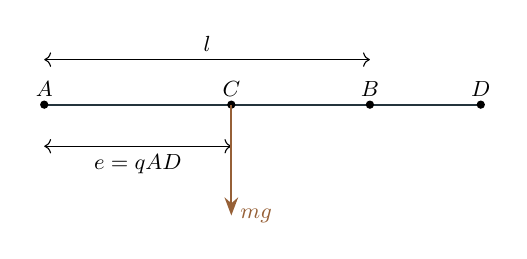
\begin{tikzpicture}[scale=.88,transform shape]
\draw[object](0,0)--(6.3,0);
\foreach \xx/\ll in {0/A,2.7/C,4.7/B,6.3/D}{\fill(\xx,0)circle(1.7pt);\node[above]at(\xx,0){$\ll$};}
\draw[<->](0,-.6)--(2.7,-.6)node[midway,below]{$e=qAD$};
\draw[<->](0,.65)--(4.7,.65)node[midway,above]{$l$};
\draw[force](2.7,0)--(2.7,-1.6)node[right]{$mg$};
\end{tikzpicture}
\figcaption{变图5.4V2\quad 重心按给定比例分整杆，内段的中点不参与这一定义。}
\end{minipage}\end{center}
\item 已知露出长度$b\ge0$，反求球内段长。均匀杆的$b=3l-8R^2/l$给出$3l^2-bl-8R^2=0$。两根中只有正根
\[
l=\frac{b+\sqrt{b^2+96R^2}}6
\]
满足长度为正。变图5.4V3 的反函数与$b(l)$一一对应，因为$\dd b/\dd l=3+8R^2/l^2>0$。$b=0$给$l=\sqrt{8/3}R$，$b\to2R$给$l\to2R$，因此非退化范围为$0\le b<2R$；严格有露出则取$b>0$。
\begin{center}\begin{minipage}{.98\linewidth}\centering
\begin{tikzpicture}[scale=.88,transform shape]
\draw[axis](0,0)--(6.5,0)node[right]{$b/R$};
\draw[axis](0,0)--(0,3.7)node[above]{$l/R$};
\draw[traj,domain=0:2,samples=80]plot({2.75*\x},{1.65*(\x+sqrt(\x*\x+96))/6});
\fill(0,2.69444)circle(1.7pt)node[right]{$\sqrt{8/3}$};
\filldraw[fill=white](5.5,3.3)circle(1.7pt)node[above]{$2$};
\end{tikzpicture}
\figcaption{变图5.4V3\quad 给定露出长度，正根在允许接触范围内单调增加。}
\end{minipage}\end{center}
\item 比较两端极限。变图5.4V4 的横轴为$l/R$，下端$\sqrt{8/3}$处$b=0$，仍有$BE^2=4R^2-l^2=4R^2/3$，且$N_A=mg/\sqrt2,\ N_B=mg/\sqrt6$。上端$l\to2R$时，$BE,CB\to0$、$\gamma\to0$，于是$N_A\to0,\ N_B\to mg$，露出段却趋向$2R$。再向下减小$l$时，均匀杆的重心条件要求$b<0$，已超出杆从$B$向外伸出的几何。
\begin{center}\begin{minipage}{.98\linewidth}\centering
\begin{tikzpicture}[scale=.88,transform shape]
\draw[axis](0,0)--(6.4,0)node[right]{$l/R$};
\draw[axis](0,0)--(0,3.7)node[above]{$b/R$};
\draw[traj,domain=1.632993:2,samples=80]plot({13*(\x-1.6)},{1.5*(3*\x-8/\x)});
\fill(.42891,0)circle(1.7pt)node[below]{$\sqrt{8/3}$};
\filldraw[fill=white](5.2,3)circle(1.7pt)node[above]{$2$};
\node[below]at(5.2,0){$2$};
\end{tikzpicture}
\figcaption{变图5.4V4\quad 下端消失的是露出段，上端趋零的是内端法向力。}
\end{minipage}\end{center}
\item 外端恰在边缘。此时$D=B$，变图5.4V5 中的$C$是$AB$中点，所以$AC=l/2$。由光滑三力共点得到$AC=2l-4R^2/l$，从而$3l^2=8R^2$。这时$BE=2R/\sqrt3$仍为正，两个支持力分别是$mg/\sqrt2$和$mg/\sqrt6$。露出段为零时，两个接触点仍可同时承担正支持力。
\begin{center}\begin{minipage}{.98\linewidth}\centering
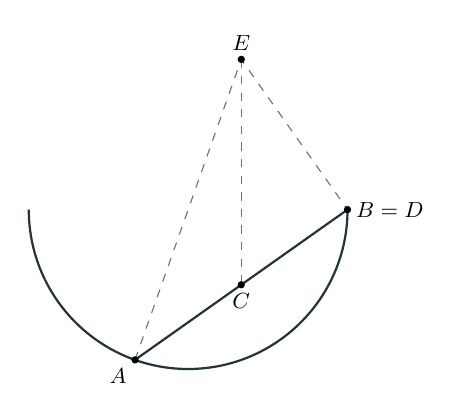
\begin{tikzpicture}[scale=.88,transform shape]
\draw[object](-2.3,0)arc(180:360:2.3);
\coordinate(A)at(-.766667,-2.16846);\coordinate(B)at(2.3,0);
\coordinate(C)at(.766667,-1.08423);\coordinate(E)at(.766667,2.16846);
\draw[object](A)--(B);\draw[guide](A)--(E)--(B);\draw[guide](E)--(C);
\foreach \pp/\pos in {A/below left,C/below,E/above}
{\fill(\pp)circle(1.5pt);\node[\pos]at(\pp){$\pp$};}
\fill(B)circle(1.5pt)node[right]{$B=D$};
\end{tikzpicture}
\figcaption{变图5.4V5\quad 零露出长度时，整杆中点在内段中点，两条法线交点仍与口缘分开。}
\end{minipage}\end{center}
\item 球内、球外线密度分别为$\lambda_i,\lambda_o$。变图5.4V6 沿杆展开，内段和外段质心距$A$分别为$l/2,l+b/2$，故
\[
AC=\frac{\lambda_i l(l/2)+\lambda_o b(l+b/2)}{\lambda_i l+\lambda_o b}=e,
\quad e=2l-4R^2/l.
\]
乘分母并整理为$b^2+2(l-e)b+(\lambda_i/\lambda_o)l(l-2e)=0$，取非负露出根
\[
b=e-l+\sqrt{(l-e)^2+(\lambda_i/\lambda_o)l(2e-l)}.
\]
由于外段质心在$B$以外，附加正质量使总重心从$l/2$向外移动，需$e\ge l/2$。若密度相同，根化为$3l-8R^2/l$。接触法向力的方向仍由$l$确定，使用总重代入主解的支持力式。
\begin{center}\begin{minipage}{.98\linewidth}\centering
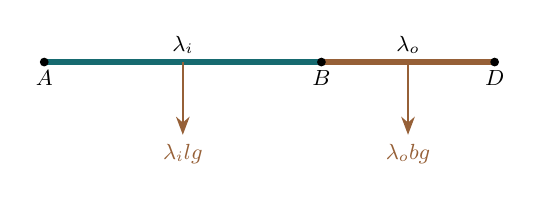
\begin{tikzpicture}[scale=.88,transform shape]
\draw[traj,line width=2pt](0,0)--(4,0);
\draw[object,line width=2pt,color=warm](4,0)--(6.5,0);
\node[above]at(2,0){$\lambda_i$};\node[above]at(5.25,0){$\lambda_o$};
\foreach \xx/\ll in {0/A,4/B,6.5/D}{\fill(\xx,0)circle(1.8pt);\node[below]at(\xx,0){$\ll$};}
\draw[force](2,0)--(2,-1.05)node[below]{$\lambda_i lg$};
\draw[force](5.25,0)--(5.25,-1.05)node[below]{$\lambda_o bg$};
\end{tikzpicture}
\figcaption{变图5.4V6\quad 两段重量作用于各自中点，用加权平均求整杆重心。}
\end{minipage}\end{center}\end{enumerate}

\clearpage

\pdfbookmark[2]{第 5 题 三圆柱堆放的摩擦下限}{q5}

\section*{第 5 题\quad 三圆柱堆放的摩擦下限}

\tagline{M-05-05}

三个半径和质量均相同的圆柱体互相接触，在水平地面上堆成两下、上一的对称构型。圆柱之间的静摩擦系数为 $\mu_1$，圆柱与地面之间为 $\mu_2$。求使三个圆柱静止所需的 $\mu_1$ 和 $\mu_2$ 的下限。

\begin{center}\begin{minipage}{\linewidth}\centering
\begin{tikzpicture}
\draw[object] (-2.4,0)--(2.4,0);\foreach \x/\y/\s in {-1/1/B,1/1/C,0/2.732/A}{\draw[object] (\x,\y)circle(1);\fill(\x,\y)circle(1.5pt);\node at(\x,\y+.25){$\s$};}\draw[guide] (-1,1)--(1,1)--(0,2.732)--cycle;\node[right]at(2,1.7){$r,m$ 相同};
\end{tikzpicture}
\figcaption{图 5.5\quad 三圆柱两两相切，圆心围成等边三角形。}
\end{minipage}\end{center}

\Needspace{5\baselineskip}

\pdfbookmark[3]{题型定位}{q5-h0}

\subsection*{题型定位}

多刚体接触与两个摩擦系数的下限。上柱通过对称简化，下柱仍须同时满足平移、转动平衡，柱间摩擦与地面摩擦分别和各自法向力比较。

整体方程中的内部接触力相消，隔离各柱后才能显出柱间摩擦及其力矩。隔离局部、保留下层法向力、用单向接触条件求最小摩擦构型，是完整解法的三个步骤。

\Needspace{5\baselineskip}

\pdfbookmark[3]{知识点}{q5-h1}

\subsection*{知识点}

\begin{itemize}
\tightlist
\item
  对称性简化受力
\item
  接触法向力与摩擦力
\item
  圆柱力矩平衡
\item
  多物体隔离法
\item
  两个摩擦系数的临界下限
\end{itemize}

三圆柱的对称性减少未知量，但每根圆柱仍须同时满足力与力矩平衡。柱间摩擦与地面摩擦的大小可以相同，法向力却不同，所以两个系数下限按各自的法向力计算。证明下限充分需构造一组满足所有平衡式和摩擦不等式的接触力。


\Needspace{5\baselineskip}

\pdfbookmark[3]{物理图像}{q5-h2}

\subsection*{物理图像}

上柱的两条法线沿圆心连线，斜向内、向上；摩擦沿公切线，斜向外、向上。对右下柱，上接触的法向力向右下，摩擦向左下，地面摩擦向左，下层相邻柱的法向力 $Q$ 向右。

解图5.5A中，对称性抵消水平合力和总力矩，剩竖直平衡；解图5.5B列下柱的平移与圆心矩。镜像平均使下层接触的切向力为零，法向力$Q$仍保留。由$Q\ge0$求$f$下限，再由两个摩擦比的单调性确定最低状态为$Q=0$。

\Needspace{5\baselineskip}

\pdfbookmark[3]{解题入口}{q5-h3}

\subsection*{解题入口}

先由上柱列 $\sqrt3N+f=mg$，再由右下柱取圆心矩得到 $f_2=f$。竖直平衡给 $N_2=3mg/2$，水平平衡保留 $Q$，结合单向接触 $Q\ge0$ 得到 $f$ 的下限。

求系数下限前应考察 $f/N$ 与 $f/N_2$ 是否随 $f$ 增大。两者都单调增加，故选择 $Q=0$ 的最小摩擦构型。柱间用$f\le\mu_1N$，地面用$f_2\le\mu_2N_2$，两项条件同时成立。

\Needspace{5\baselineskip}

\pdfbookmark[3]{标准解法}{q5-h4}

\subsection*{标准解法}

\textbf{上柱与下柱的隔离受力。}设每柱质量为 $m$。上柱与每个下柱之间的法向力为 $N$、摩擦力为 $f$；每个下柱受地面支持力 $N_2$、向内的摩擦力 $f_2$。保留下层两柱之间的法向力 $Q$。镜面对称使这个竖直接触面的切向力为零，但法向力仍可以存在。
\begin{center}\begin{minipage}{\linewidth}\centering
\begin{tikzpicture}
\draw[object](0,0)circle(1);
\draw[force](-.5,-.866025404)--(.05,.086602540)node[above right]{$N$};
\draw[force](.5,-.866025404)--(-.05,.086602540)node[above left]{$N$};
\draw[force](-.5,-.866025404)--(-.755255888,-.718653348)node[above left]{$f$};
\draw[force](.5,-.866025404)--(.755255888,-.718653348)node[above right]{$f$};
\draw[force](0,0)--(0,-2.2)node[below]{$mg$};
\node at(0,1.45){上圆柱};
\end{tikzpicture}
\figcaption{解图5.5A\quad 以最低摩擦状态的大小比例绘受力；两侧法向力和摩擦的水平分量分别相消。}
\end{minipage}\end{center}
解图5.5A把上柱单独隔离，两个接触点的法线均沿圆心连线；解图5.5B再隔离一个下柱，保留它与另一根下柱之间的水平推力$Q$。这两张图使用同一对作用与反作用，因而柱间摩擦$f$在两柱上的方向相反；下柱绕自身圆心取矩时，法向力不贡献力矩，才能把地面摩擦$f_2$与$f$联系起来。

圆心连线与水平成 $60^\circ$，上柱两侧法向力均斜向内、向上，摩擦力斜向外、向上。上柱竖直平衡为
\[
 2N\sin60^\circ+2f\cos60^\circ=mg,
 \qquad \sqrt3N+f=mg.\tag{1}
\]
两侧水平分量和力矩因对称抵消。
\begin{center}\begin{minipage}{\linewidth}\centering
\begin{tikzpicture}
\draw[object](0,1)circle(1);\draw[object](-1.5,0)--(1.6,0);
\draw[force](-.5,1.866025404)--(.05,.913397460)node[below right]{$N$};
\draw[force](-.5,1.866025404)--(-.755255888,1.718653348)node[above left]{$f$};
\fill(-1,1)circle(1.5pt);\draw[guide](-1,1)--(-1.65,1.45);
\node[above left]at(-1.65,1.45){$Q=0$（临界）};
\draw[force](0,0)--(-.294744112,0)node[below left]{$f_2$};
\draw[force](0,0)--(0,3.3)node[above right]{$N_2$};
\draw[force](0,1)--(0,-1.2)node[below]{$mg$};
\node at(2.6,1.5){右下圆柱};
\end{tikzpicture}
\figcaption{解图5.5B\quad 最低摩擦临界状态取$Q=0$；一般平衡仍保留$Q\geq0$，各实际作用点用于圆心矩。}
\end{minipage}\end{center}
\textbf{下柱还须满足转动平衡。}取右下柱。地面法向力、重力、圆柱间法向力都通过圆心，不产生力矩；上接触摩擦与地面摩擦有相等力臂 $r$，转向相反，故
\[
 rf-rf_2=0,\qquad f_2=f.\tag{2}
\]
竖直、水平平衡分别是
\begin{align*}
 N_2&=mg+N\sin60^\circ+f\cos60^\circ=\frac32mg,\tag{3}\\
 \frac N2-\frac{\sqrt3}2f+Q-f_2&=0.\tag{4}
\end{align*}
从(1)、(2)、(4)得到
\[
 N=\frac{mg-f}{\sqrt3},\qquad
 Q=\frac{(4+2\sqrt3)f-mg}{2\sqrt3}.
\]
下层两柱之间是单侧接触，法向力取$Q\ge0$，因此
\[
 f\ge f_*:=\frac{mg}{4+2\sqrt3}
 =\frac{2-\sqrt3}{2}mg.
\]
$f$的最小值使$Q$恰为零，两下柱此时保持几何相切。

\textbf{两个摩擦下限同时取到。}在 $0\le f<mg$ 内，$N>0$，所需比值
\[
 \frac fN=\frac{\sqrt3 f}{mg-f},\qquad
 \frac{f_2}{N_2}=\frac{2f}{3mg}
\]
都随 $f$ 增大。因此使两个摩擦系数最小的构型是 $f=f_*$、$Q=0$。由(1)得 $N=mg/2$，从而
\[
 \boxed{\mu_1\ge2-\sqrt3},\qquad
 \boxed{\mu_2\ge\frac{2-\sqrt3}{3}}.
\]
数值约为 $0.26795$ 和 $0.08932$。这两个条件不仅必要，而且充分：取上述 $N,f,N_2,f_2,Q$，所有平衡方程都成立，且各接触力均非负、各摩擦力均不超限。地面摩擦大小虽与柱间摩擦相同，支持力却是三倍，所以两种摩擦系数下限不能相等。
\subsubsection*{为什么可以在对称受力中求下限}
若已有一组可行接触力，将它关于竖直中线镜像，就得到另一组可行解。
两组的平均也满足每根圆柱的合力、力矩方程。
对同一接触，库仑约束$|f|\leq\mu N$及$N\geq0$构成凸集合，
所以平均后的接触力仍满足各摩擦上限与单侧接触。
这组平均解左右对称，下层两柱接触处的竖直切向力与其镜像相反，平均为零，
水平法向力$Q$则保留。
因此使用对称方程没有排除任何“存在平衡”的材料参数，所求下限仍是完整下限。

\subsubsection*{给定两种材料时的对称接触力}
前面以$f$参数化平衡力，两个摩擦不等式分别给
\[
\frac{\sqrt3 f}{mg-f}\leq\mu_1
\quad\Longrightarrow\quad
f\leq\frac{\mu_1mg}{\sqrt3+\mu_1},
\]
\[
\frac{2f}{3mg}\leq\mu_2
\quad\Longrightarrow\quad
f\leq\frac32\mu_2mg.
\]
结合$Q\geq0$，可行区间为
\[
\boxed{\frac{mg}{4+2\sqrt3}\leq f\leq
\min\left(\frac{\mu_1mg}{\sqrt3+\mu_1},\frac32\mu_2mg\right)}.
\]
只要此区间非空，代回$N=(mg-f)/\sqrt3$、$N_2=3mg/2$、
$f_2=f$和$Q$的表达式，就能构造完整静力解。
区间非空的条件恰为两个系数分别不小于前述下限。
提高地面摩擦系数不能补偿不足的柱间系数，反之亦然；
两个约束限制的是同一$f$的不同上界。

在最低系数的临界状态，
\[
N=\frac{mg}{2},\quad f=f_2=\frac{2-\sqrt3}{2}mg,\quad
N_2=\frac{3mg}{2},\quad Q=0.
\]
在摩擦系数取下限时，下层两柱刚好相切，接触法向力 $Q=0$。
当材料系数更大时，静摩擦只需落在可行区间，不必把每个接触都取成$f=\mu N$。


\Needspace{5\baselineskip}

\pdfbookmark[3]{关键洞察}{q5-h5}

\subsection*{关键洞察}

摩擦同时控制平移与转动。右下柱圆心矩使柱间摩擦和地面摩擦大小相等，但法向支持力不同，因此两个系数下限不同。

下层接触法向力越大，外推趋势越强，所需摩擦也越大。保留 $Q$ 再求最小值，既补全受力图，又说明最低摩擦状态下两下柱只保持几何相切、没有相互压紧。

\Needspace{5\baselineskip}

\pdfbookmark[3]{易错点}{q5-h6}

\subsection*{易错点}

\begin{itemize}\item 接触法线沿圆心连线，摩擦沿公切线，两者互相垂直。\item 对称只消掉整体水平分量，不消掉局部摩擦。\item 下柱还需列圆心矩，才能得到 $f_2=f$。\item 保留下层法向力$Q$，用$Q\ge0$确定$f$的下限。\item 柱间摩擦配法向力$N$及$\mu_1$，地面摩擦配$N_2$及$\mu_2$。\item 同一柱间接触的力在两根柱上反向，在各自接触点标出绕圆心的转向。\end{itemize}

\Needspace{5\baselineskip}

\pdfbookmark[3]{课堂讲解建议}{q5-h7}

\subsection*{课堂讲解建议}

分两张图讲：上柱先给一个竖直方程，右下柱再给完整三方程。要求学生指出每个摩擦实际作用点，并对圆心说明转向。法向力通过圆心，没有力矩，摩擦才联系起上接触与地面。

在下柱间的接触点画出$Q$，问“接触力为正给$f$什么范围？”由水平式得到$f\ge f_*$。再分别让柱间或地面光滑，请学生指出哪一条水平或圆心矩方程失去所需的力。

若学生质疑静摩擦力也可不对称，说明存在性问题可用镜像平均选取对称解，
关键依据是平衡方程线性、库仑允许区间为凸集。
再写出完整$f$区间，让学生分别指向柱间和地面给出的两个上界；只有下界低于这两个上界，才有静止解。

\Needspace{5\baselineskip}

\pdfbookmark[3]{变式训练}{q5-h8}

\subsection*{变式训练}

\begin{enumerate}
\item 柱间光滑，地面再粗糙能否静止？变图5.5V1 上柱竖直平衡给$N=mg/\sqrt3$。对一个下柱取圆心矩，只有地面摩擦有力矩，故$f_2=0$。该下柱水平方程变为$N/2+Q=0$，而两项均非负且$N>0$，无静力解。地面的摩擦能力虽可很大，转动平衡仍要求实际摩擦为零。
\begin{center}\begin{minipage}{.98\linewidth}\centering
\begin{tikzpicture}[scale=.88,transform shape]
\draw[object](0,1)circle(1);\draw[object](-1.6,0)--(2,0);
\draw[force](-.5,1.866)--(.1,.827)node[right]{$N$};
\draw[force](-1,1)--(-.1,1)node[above]{$Q$};
\draw[guide](0,0)--(0,1);\node[right]at(.3,2.1){$f=0$};
\node[below]at(.1,-.35){圆心矩给$f_2=0$};
\end{tikzpicture}
\figcaption{变图5.5V1\quad 两个向外的水平作用得不到平衡，地面摩擦受力矩约束。}
\end{minipage}\end{center}
\item 地面足够粗糙，但柱间$\mu_1$低于下限。单侧接触给$f\ge f_*=mg/(4+2\sqrt3)$，而柱间摩擦给$f\le\mu_1mg/(\sqrt3+\mu_1)$。变图5.5V2 取$\mu_1=0.20$，上界约$0.10352mg$，小于$f_*\simeq0.13397mg$，可行区间为空。材料系数减小使下柱平移和转动的摩擦要求无法同时满足。各柱随后怎样平移、转动，由接触状态和动力学方程决定。
\begin{center}\begin{minipage}{.98\linewidth}\centering
\begin{tikzpicture}[scale=.88,transform shape]
\draw[axis](0,0)--(7,0)node[right]{$f/(mg)$};
\draw[object,very thick](0,.7)--(3.1055,.7);
\draw[traj,->](4.0192,1.5)--(6.7,1.5);
\draw[guide](3.1055,0)--(3.1055,1.1);
\draw[guide](4.0192,0)--(4.0192,1.8);
\node[below]at(3.1055,0){$0.10352$};\node[above]at(4.0192,1.5){$f_*/mg$};
\node at(1.45,1.05){摩擦上界};\node at(5.7,1.85){单侧接触下界};
\end{tikzpicture}
\figcaption{变图5.5V2\quad 柱间摩擦上界低于所需下界，两者没有交集。}
\end{minipage}\end{center}
\item 明确一种四柱排列：三柱在底层，第四柱压在左边相邻两柱上，如变图5.5V3 。最右底柱与左邻的接触力含向右法向力$Q_{23}$和有符号的向上摩擦$s$，地面有水平力$h$与法向力$N_3$。平移、圆心矩分别给
\[
Q_{23}+h=0,\quad N_3+s=mg,\quad rh-rs=0.
\]
因此$s=h=-Q_{23}$、$N_3=mg+Q_{23}$。柱间条件要求$Q_{23}\le\mu_1Q_{23}$，所以在$\mu_1<1$分支上只能取$Q_{23}=0$。此时右侧附加柱只由地面承重，左侧三柱仍有本题两个下限，特别是最小柱间系数仍为$2-\sqrt3$。若$\mu_1\ge1$，该额外接触可传递水平力，同时还需$Q_{23}\le\mu_2(mg+Q_{23})$，并将它对中间下柱的反向作用加入三柱方程。四柱排列与各接触的摩擦方向共同决定完整可行域。
\begin{center}\begin{minipage}{.98\linewidth}\centering
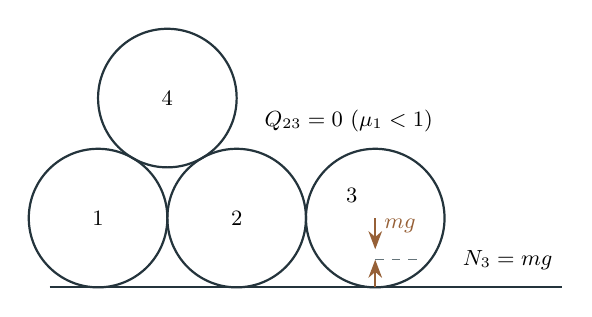
\begin{tikzpicture}[scale=.88,transform shape]
\draw[object](-1.7,0)--(5.7,0);
\foreach \xx/\yy/\ll in {-1/1/1,1/1/2,0/2.732/4}{\draw[object](\xx,\yy)circle(1);\node at(\xx,\yy){$\ll$};}
\draw[object](3,1)circle(1);
\node at(2.66,1.32){$3$};
\node[anchor=west]at(1.28,2.40){$Q_{23}=0\ (\mu_1<1)$};
\draw[force](3,0)--(3,.40);\draw[guide](3,.40)--(3.6,.40);\node[anchor=west]at(4.14,.40){$N_3=mg$};
\draw[force](3,1)--(3,.55)node[right,pos=.24]{$mg$};
\end{tikzpicture}
\figcaption{变图5.5V3\quad 在最小柱间摩擦分支上，额外底柱的侧法向力和侧摩擦同时为零。}
\end{minipage}\end{center}
\item 只画方向并写对应分量。变图5.5V4 隔离右下柱：上方接触法向力向右下、摩擦向左下，地面摩擦向左，邻柱法向力$Q$向右，地面支持力向上，重力向下。上接触法向与摩擦的点积为零。水平式为$N/2-\sqrt3 f/2+Q-f_2=0$，竖直式为$N_2=mg+\sqrt3N/2+f/2$，圆心矩为$r(f-f_2)=0$。这三式把各箭头逐项转为平衡条件。
\begin{center}\begin{minipage}{.98\linewidth}\centering
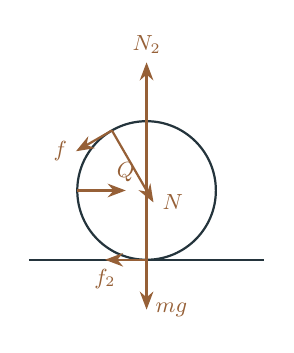
\begin{tikzpicture}[scale=.88,transform shape]
\draw[object](0,1)circle(1);\draw[object](-1.7,0)--(1.7,0);
\draw[force](-.5,1.866)--(.1,.827)node[right]{$N$};
\draw[force](-.5,1.866)--(-1.0196,1.566)node[left]{$f$};
\draw[force](0,0)--(-.6,0)node[below]{$f_2$};
\draw[force](0,0)--(0,2.85)node[above]{$N_2$};
\draw[force](0,1)--(0,-.72)node[right]{$mg$};
\draw[force](-1,1)--(-.3,1)node[above]{$Q$};
\end{tikzpicture}
\figcaption{变图5.5V4\quad 每条摩擦力沿对应接触切线，法向力沿圆心或竖直方向。}
\end{minipage}\end{center}
\item 只保留上柱与一个下柱，仍沿原来的斜向连心线接触。变图5.5V5 的两柱总重心位于连心线中点，其铅垂线距地面接触点水平$r/2$。整体水平外力为零要求地面摩擦为零，地面支持力过底柱圆心；重力对地面接触点的力矩则为$2mg(r/2)=mgr>0$。因此此二柱倾斜构型没有静止解。加墙后会有新的外力矩，应从新的整体外力重新列式。
\begin{center}\begin{minipage}{.98\linewidth}\centering
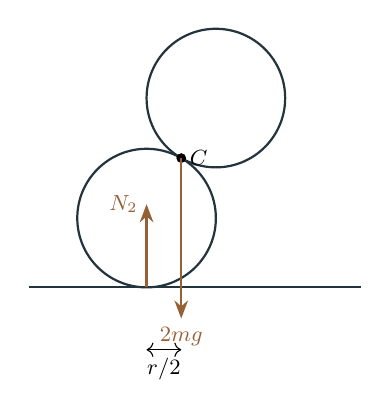
\begin{tikzpicture}[scale=.88,transform shape]
\draw[object](-1.7,0)--(3.1,0);\draw[object](0,1)circle(1);\draw[object](1,2.732)circle(1);
\fill(.5,1.866)circle(2pt)node[right]{$C$};
\draw[force](.5,1.866)--(.5,-.45)node[below]{$2mg$};
\draw[force](0,0)--(0,1.2)node[left]{$N_2$};
\draw[<->](0,-.9)--(.5,-.9)node[midway,below]{$r/2$};
\end{tikzpicture}
\figcaption{变图5.5V5\quad 两柱总重力的作用线偏离唯一地面支持线。}
\end{minipage}\end{center}
\item 比较作用与反作用。变图5.5V6 在同一柱间接触点画两组反向箭头。上柱受到下柱的$N,f$，下柱受到上柱的$-N,-f$，两组作用于不同圆柱；把两柱组成整体时，它们的合力与合力矩同时相消。地面摩擦的另一作用对象是地面。下柱圆心矩给$f_2=f$，这是一条平衡关系，二者的作用点和相互作用对象各有对应位置。
\begin{center}\begin{minipage}{.98\linewidth}\centering
\begin{tikzpicture}[scale=.88,transform shape]
\draw[object](0,0)circle(1);\draw[object](1,1.732)circle(1);
\coordinate(P)at(.5,.866);
\draw[force](P)--(1,1.732)node[right]{$N$};
\draw[force](P)--(0,0)node[below]{$-N$};
\draw[force](P)--(-.1928,1.266)node[left]{$f$};
\draw[force](P)--(1.1928,.466)node[right]{$-f$};
\fill(P)circle(2pt);\node[above]at(1,2.95){柱间接触};
\end{tikzpicture}
\figcaption{变图5.5V6\quad 作用反作用在相同接触处反向，分别作用于两根柱。}
\end{minipage}\end{center}\end{enumerate}

\clearpage

\pdfbookmark[2]{第 6 题 斜木板上三球的支承}{q6}

\section*{第 6 题\quad 斜木板上三球的支承}

\tagline{M-05-06}

均匀木板 $AB$ 长 $L=100\,\mathrm{cm}$，重 $2G$。$A$ 端铰接在竖直墙上，$B$ 端由水平轻绳拉住，木板与墙的夹角为 $60^\circ$。三个相同小球沿木板排列，彼此接触且都接触木板；最左球还接触墙。每球半径 $R=10\,\mathrm{cm}$，重 $G$。球与墙、木板以及球之间均光滑。求水平绳的张力 $T$。

\begin{center}\begin{minipage}{\linewidth}\centering
\begin{tikzpicture}
\coordinate(A)at(0,0);\coordinate(B)at(5.196152423,3);
\coordinate(E)at(.9,.519615242);\coordinate(F)at(1.939230485,1.119615242);
\coordinate(K)at(2.978460969,1.719615242);\coordinate(D)at(1.679422863,.969615242);
\draw[object](0,-.3)--(0,3.5);\draw[object](A)--(B)--(0,3);
\foreach \x/\y in {.6/1.039230485,1.639230485/1.639230485,2.678460969/2.239230485}
{\draw[object](\x,\y)circle(.6);}
\draw(0,.7)arc(90:30:.7);\node at(.45,.78){$60^\circ$};
\node[below]at(A){$A$};\node[right]at(B){$B$};
\node[above]at(3.7,3){水平绳};\node[below right]at(3.7,1.9){$L=10R$};
\end{tikzpicture}
\figcaption{图5.6\quad 三球与板、墙接触；木板长度及球半径按$L:R=10:1$绘制。}
\end{minipage}\end{center}

\Needspace{5\baselineskip}

\pdfbookmark[3]{题型定位}{q6-h0}

\subsection*{题型定位}

光滑多球支承与木板端力计算。三球整体法消去球间力，用外力的平移与力矩确定板合力的大小和作用线，再对木板取铰链矩。

三球重力合力通过中球，墙力对中球有力矩，板支持力的合力作用线因而向左偏移。可用三球整体取矩求偏移，也可按三个不同的板支持力加权求作用点，再对木板取矩求张力。

\Needspace{5\baselineskip}

\pdfbookmark[3]{知识点}{q6-h1}

\subsection*{知识点}

\begin{itemize}
\tightlist
\item
  光滑接触支持力方向
\item
  三球整体受力
\item
  等效支持力作用线
\item
  木板绕铰链力矩平衡
\item
  反作用力传递到支承物
\end{itemize}

对三球与木板整体取矩可消去球间内力，逐球隔离则给出木板所受各法向力。球的接触方向由连心线给定，铰链反力一般含水平、竖直两分量。把球对板的压力合成到木板上时，沿原作用线取反向，并按这条线到铰链的距离求矩。


\Needspace{5\baselineskip}

\pdfbookmark[3]{物理图像}{q6-h2}

\subsection*{物理图像}

三个球沿板相切，圆心共线并与板平行。三球整体受墙力、板上各法向力的合力和总重；内部球间力抵消。总重通过中球中心，板支持合力的位置则由它与墙力的力矩平衡确定。

解图5.6A中，墙力相对中球中心有力矩，板合力作用线向左偏移$R/2$，与这份墙力矩相抵。解图5.6B再把这个合力反向施加在木板上。铰链传递两个方向的力，而端部绳只能水平拉；选 $A$ 为矩心可消去铰链的两个分量。

\Needspace{5\baselineskip}

\pdfbookmark[3]{解题入口}{q6-h3}

\subsection*{解题入口}

对三球整体先列两条平移平衡，求墙力 $N_1$ 与板合力 $N_2$；再以中球中心取矩求合力相对垂足的偏移 $R/2$。左球的接触几何给出 $AE=\sqrt3R$。

得到 $AD=(\sqrt3+3/2)R$ 后，对木板绕 $A$ 取矩。应先把各力臂写成 $L\sin30^\circ$、$(L/2)\cos30^\circ$、$AD$，再代数计算。逐球法分别求三个板支持力，再按各自力矩加权，得到同一合力位置。

\Needspace{5\baselineskip}

\pdfbookmark[3]{标准解法}{q6-h4}

\subsection*{标准解法}

\textbf{先研究三个球组成的整体。}板与水平成 $\beta=30^\circ$。整体重力 $3G$ 通过中球中心 $C$；墙对左球的支持力 $N_1$ 水平向右；木板对三球的法向力合为 $N_2$，垂直木板。球间接触力都是内力。
\begin{center}\begin{minipage}{\linewidth}\centering
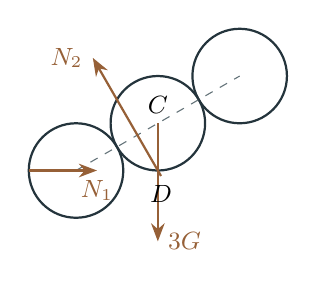
\begin{tikzpicture}
\coordinate(A)at(0,0);\coordinate(B)at(5.196152423,3);
\coordinate(E)at(.9,.519615242);\coordinate(F)at(1.939230485,1.119615242);
\coordinate(K)at(2.978460969,1.719615242);\coordinate(D)at(1.679422863,.969615242);
\foreach \x/\y in {.6/1.039230485,1.639230485/1.639230485,2.678460969/2.239230485}
{\draw[object](\x,\y)circle(.6);}
\draw[guide](.6,1.039230485)--(2.678460969,2.239230485);
\draw[force](0,1.039230485)--(.866025404,1.039230485)node[below]{$N_1$};
\draw[force](D)--(.813397459,2.469615242)node[left]{$N_2$};
\draw[force](1.639230485,1.639230485)--(1.639230485,.139230485)node[right]{$3G$};
\node[above]at(1.639230485,1.639230485){$C$};\node[below]at(D){$D$};
\end{tikzpicture}
\figcaption{解图5.6A\quad 墙力对$C$逆时针，板合力对$C$顺时针；$D$在中球垂足左侧。}
\end{minipage}\end{center}
解图5.6A将三球作为整体，其竖直、水平平衡给出
\[
 N_2\cos30^\circ=3G,\qquad
 N_1=N_2\sin30^\circ,
\]
所以 $N_2=2\sqrt3G$，$N_1=\sqrt3G$。

\textbf{求板上合力的作用点。}设左球中心在板上的垂足为 $E$，中球中心的垂足为 $F$，合力作用点为 $D$。由于三球都接触板，相邻圆心距为 $2R$，$EF=2R$。墙与板夹角为 $60^\circ$，左球中心在该夹角的角平分线上，故
\[
 AE=R\cot30^\circ=\sqrt3R.
\]
墙力的作用线通过左球中心；它到 $C$ 的竖直距离为 $2R\sin30^\circ=R$。对整体关于$C$取矩，$N_1$向右且作用线在$C$下方，产生逆时针力矩；板合力作用点在$F$左侧时产生顺时针力矩，二者相抵。令 $FD=x$，则
\[
 N_2x=N_1R,\qquad x=\frac R2.
\]
因此
\[
 AD=AE+EF-FD=\left(\sqrt3+\frac32\right)R.
\]
\textbf{再研究木板。}解图5.6B中，球给木板的压力大小为 $N_2$、方向垂直板向下右，作用于 $D$。板重 $2G$ 作用于中点。铰链可同时提供 $A_x,A_y$，对 $A$ 取矩可一并消去。
\begin{center}\begin{minipage}{\linewidth}\centering
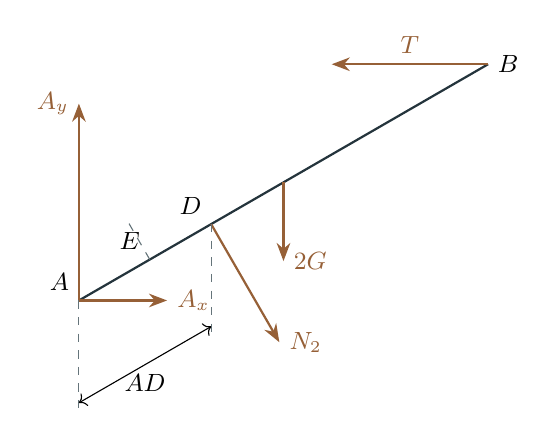
\begin{tikzpicture}
\coordinate(A)at(0,0);\coordinate(B)at(5.196152423,3);
\coordinate(E)at(.9,.519615242);\coordinate(F)at(1.939230485,1.119615242);
\coordinate(K)at(2.978460969,1.719615242);\coordinate(D)at(1.679422863,.969615242);
\draw[object](A)--(B);
\draw[force](B)--(3.210511777,3)node[midway,above]{$T$};
\draw[force](D)--(2.545448267,-.530384758)node[right]{$N_2$};
\draw[force](2.598076211,1.5)--(2.598076211,.5)node[right]{$2G$};
\draw[force](A)--(0,2.5)node[left]{$A_y$};
\draw[force](A)--(1.119615242,0)node[right]{$A_x$};
\draw[guide](E)--(.6,1.039230485);\node[above left]at(E){$E$};
\node[above left]at(D){$D$};\node[above left]at(A){$A$};\node[right]at(B){$B$};
\draw[guide](A)--(0,-1.4);\draw[guide](D)--(1.679422863,-.430384758);
\draw[<->](0,-1.3)--(1.679422863,-.330384758)node[midway,below]{$AD$};
\end{tikzpicture}
\figcaption{解图5.6B\quad 球对板的压力沿同一作用线反向；铰链两反力均保留，力矩臂按实际$L:R$绘制。}
\end{minipage}\end{center}
张力的力臂是 $L\sin30^\circ$，板重的力臂为 $(L/2)\cos30^\circ$，而球压力垂直板，力臂直接为 $AD$。故
\[
 TL\sin30^\circ=N_2AD+2G\frac L2\cos30^\circ.
\]
代入 $R/L=1/10$，逐项化简：
\begin{align*}
 \frac{TL}{2}
 &=2\sqrt3G\left(\sqrt3+\frac32\right)R
   +\frac{\sqrt3}{2}GL\\
 &=(6+3\sqrt3)GR+\frac{\sqrt3}{2}GL,\\
 T&=\left[2(6+3\sqrt3)\frac RL+\sqrt3\right]G
 =\boxed{\frac{6+8\sqrt3}{5}G}\approx3.97128G.
\end{align*}
\textbf{三个板支持力的合力位置。}从右球向左球依次列沿板方向平衡，球间压力依次为 $G/2,G$；三个球所受板支持力，从左到右为 $\sqrt3G,\sqrt3G/2,\sqrt3G/2$。它们作用于 $E,E+2R,E+4R$，加权平均位置为
\[
 AD=AE+\frac{(\sqrt3G/2)2R+(\sqrt3G/2)4R}{2\sqrt3G}
 =AE+\frac32R.
\]
\begin{center}\begin{minipage}{\linewidth}\centering
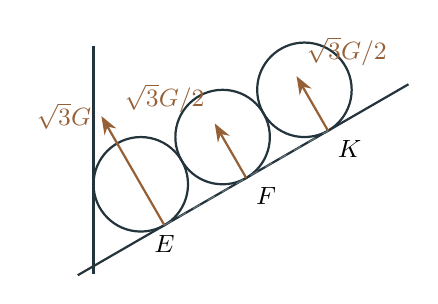
\begin{tikzpicture}
\coordinate(A)at(0,0);\coordinate(B)at(5.196152423,3);
\coordinate(E)at(.9,.519615242);\coordinate(F)at(1.939230485,1.119615242);
\coordinate(K)at(2.978460969,1.719615242);\coordinate(D)at(1.679422863,.969615242);
\draw[object](-.2,-.115470054)--(4,2.309401077);
\draw[object](0,-.1)--(0,2.8);
\foreach \x/\y in {.6/1.039230485,1.639230485/1.639230485,2.678460969/2.239230485}
{\draw[object](\x,\y)circle(.6);}
\draw[force](E)--(.1,1.905255888)node[left]{$\sqrt3G$};
\draw[force](F)--(1.539230485,1.812435565)node[above left]{$\sqrt3G/2$};
\draw[force](K)--(2.578460969,2.412435565)node[above right]{$\sqrt3G/2$};
\node[below]at(E){$E$};\node[below right]at(F){$F$};\node[below right]at(K){$K$};
\draw[guide](E)--(K);
\end{tikzpicture}
\figcaption{解图5.6C\quad 仅画待合成的三个法向力，作用点沿板相隔$2R$；逐球其他力由对应分量方程列出。}
\end{minipage}\end{center}
解图5.6C 把三个法向支持力按各自作用点合成，得到与整体取矩相同的作用点。木板的平移平衡给出铰链的竖直分力 $A_y=5G$ 和水平分力 $A_x=T-\sqrt3G$。
\subsubsection*{各球的法向力和切向平衡}
以$\vect t$沿板向右上、$\vect n$垂直板向左上，
三个球从左到右记为1、2、3，球间压力记为$P_{12},P_{23}$。
球间连心线与板平行，所以它们只在切向方程中出现。
先从最右球开始：
\[
P_{23}=G\sin30^\circ=\frac G2,\qquad
N_K=G\cos30^\circ=\frac{\sqrt3}2G.
\]
中球受到左球向右上的推力与右球向左下的推力，故
\[
P_{12}-P_{23}=G\sin30^\circ,\qquad
N_F=G\cos30^\circ,
\]
得到$P_{12}=G$、$N_F=\sqrt3G/2$。
左球另受水平墙力$N_1$，它的切向分量向板上，法向分量向板内：
\[
N_1\cos30^\circ-P_{12}-G\sin30^\circ=0,
\]
\[
N_E-N_1\sin30^\circ-G\cos30^\circ=0.
\]
逐式代入，恢复$N_1=\sqrt3G$、$N_E=\sqrt3G$。
所有球间压力与板支持力都为正，因此整体合成所使用的接触构型可以实现。
各球所受的接触法向力和重力都通过各自的圆心，对圆心的总力矩为零。

解图5.6C中，从左至右各垂足沿板的距离为
$AE,AE+2R,AE+4R$。三个法向力大小不同，合力位置用它们的大小作权重。三球质量相同，所以总重心位于中球的球心。
最右接触点距铰链为$(\sqrt3+4)R<10R=L$，
三个板接触点都在有限木板内，合力点$D$也在最左、最右接触点之间。

\subsubsection*{木板和三球整体的力矩}
这一选取会消去全部球板内力，外力中仍须保留墙对最左球的水平支持力。
令铰链$A$为坐标原点，三球中心的横坐标依次为
\[
R,\quad R+2R\cos30^\circ,\quad R+4R\cos30^\circ,
\]
墙力作用线的高度为$\sqrt3R$。
以逆时针为正，水平向右的墙力对$A$产生顺时针力矩，
球重和板重也产生顺时针力矩，只有$B$处向左的绳拉力产生逆时针力矩。
因此
\[
\begin{aligned}
TL\sin30^\circ
&=2G\frac L2\cos30^\circ+G(3R+6R\cos30^\circ)+N_1\sqrt3R\\
&=\frac{\sqrt3}{2}GL+(6+3\sqrt3)GR.
\end{aligned}
\]
与木板单独取矩中的$N_2AD$完全相同，故仍得$T=(6+8\sqrt3)G/5$。
墙力是板球整体的外力，它关于$A$的力矩为$3GR$，保留在整体矩方程中。

再回到三球重心$C$取矩：墙力作用线在$C$下方，水平向右，
所以它对$C$是逆时针；$D$在中球垂足$F$的左侧，
向左上的板合力对$C$是顺时针。
两力矩相抵才有$N_2FD=N_1R$。
同一墙力关于$A$和$C$的转向不同，因为两矩心分处其作用线两侧；
力矩方向由选定矩心与力的作用线共同决定。


\Needspace{5\baselineskip}

\pdfbookmark[3]{关键洞察}{q6-h5}

\subsection*{关键洞察}

整体法消去内部球间力，但不自动确定板合力的作用位置；这一步仍由整体力矩平衡决定。若直接把 $3G$ 施加在木板上，会同时错掉方向和力臂。

逐球法给出的支持力不相等，左球多承受墙力向板内的分量。因此板压力的加权位置偏向左球，与整体关于中球中心的取矩结果一致。

\Needspace{5\baselineskip}

\pdfbookmark[3]{易错点}{q6-h6}

\subsection*{易错点}

\begin{itemize}\item 三球的重力合力通过中球，板支持力合力不一定通过其垂足。\item $AE=R\cot30^\circ=\sqrt3R$，由左球中心在墙板夹角平分线上得到。\item 板对球的支持力向左上，球对板的压力沿同一法线向右下。\item 水平绳力臂为 $L\sin30^\circ$，板重力臂为 $(L/2)\cos30^\circ$。\item 铰链传递水平与竖直两个分量，板的竖直平衡给$A_y=5G$。\item 各球的板支持力大小不同，合力位置由整体力矩或按各支持力加权得到。\end{itemize}

\Needspace{5\baselineskip}

\pdfbookmark[3]{课堂讲解建议}{q6-h7}

\subsection*{课堂讲解建议}

先在解图5.6A用整体法求$N_1,N_2$，再问“墙力对中球中心朝哪个方向转？”由逆时针矩让学生把板合力作用点移到中球垂足左侧，画出反向矩，再求$x=R/2$。

从三球换到木板时，把解图5.6B 中球对板的压力画成与板对球的支持力相反。标出三支外力对铰链的力臂，再求张力。问“铰链的竖直分力承担哪些重量？”木板与三球共重 $5G$，因此 $A_y=5G$。最后按解图5.6C 的三个支持力加权求作用点 $D$，与整体力矩所得位置相同。

固定矩心$C$时，墙力在其下方向右，转向为逆时针；板合力在左侧产生顺时针矩。
换成矩心$A$，同一墙力却为顺时针，要求学生把两条力矩分别用坐标或力臂符号算出。
最后将板与三球合成整体，保留墙的外力矩，独立恢复张力；墙力在该矩方程中贡献 $3GR$ 的顺时针矩。

\Needspace{5\baselineskip}

\pdfbookmark[3]{变式训练}{q6-h8}

\subsection*{变式训练}

\begin{enumerate}
\item 改成两个相同球，板重仍为$2G$。变图5.6V1 左球垂足距铰链$AE=\sqrt3R$；墙力为$2G\tan\beta$，左、右球的板支持力分别为$G\cos\beta+2G\sin^2\beta/\cos\beta$、$G\cos\beta$。故总法向力$N_\Sigma=2G/\cos\beta$，加权位置
\[
AD=AE+\frac{(G\cos\beta)2R}{2G/\cos\beta}
=\sqrt3R+R\cos^2\beta.
\]
代$\beta=30^\circ$，对板取矩得
\[
T=\left[\frac{4(\sqrt3+3/4)R}{L\cos30^\circ}+\cot30^\circ\right]G
=\left(\frac45+\frac{6\sqrt3}{5}\right)G .
\]
这里仍用$R/L=1/10$。
\begin{center}\begin{minipage}{.98\linewidth}\centering
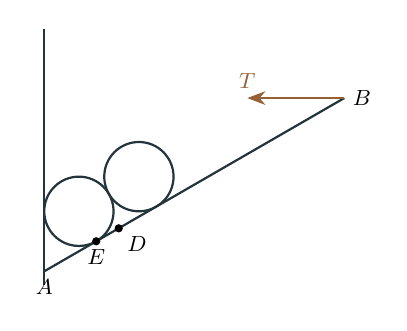
\begin{tikzpicture}[scale=.88,transform shape]
\draw[object](0,-.2)--(0,3.5000000);\draw[object](0,0)--(4.3301270,2.5000000);
\draw[object](0.5000000,0.8660254)circle(.5);
\draw[object](1.3660254,1.3660254)circle(.5);
\fill (0.75,0.4330127) circle(1.7pt) node[below] {$E$};
\fill (1.07475953,0.6205127) circle(1.7pt) node[below right] {$D$};
\draw[force](4.3301270,2.5000000)--++(-1.4,0)node[above]{$T$};\node[below]at(0,0){$A$};\node[right]at(4.3301270,2.5000000){$B$};
\end{tikzpicture}
\figcaption{变图5.6V1\quad 两球时右球支持力的权重使合力落在左球垂足右侧 $3R/4$。}
\end{minipage}\end{center}
\item 将板重从$2G$减为$G$。三球的位置与受力均未变，因此球对板的总压力矩$N_\Sigma AD$保持原值。变图5.6V2 的板重只在板中点向下。由$TL\sin30^\circ=N_\Sigma AD+W(L/2)\cos30^\circ$，板重减少$G$使张力减少
\[
\Delta T=\frac G2\cot30^\circ=\frac{\sqrt3}2G.
\]
新张力为$(6/5+11\sqrt3/10)G$。
\begin{center}\begin{minipage}{.98\linewidth}\centering
\begin{tikzpicture}[scale=.88,transform shape]
\draw[object](0,-.2)--(0,3.5000000);\draw[object](0,0)--(4.3301270,2.5000000);
\draw[object](0.5000000,0.8660254)circle(.5);
\draw[object](1.3660254,1.3660254)circle(.5);
\draw[object](2.2320508,1.8660254)circle(.5);
\draw[force](4.3301270,2.5000000)--++(-1.4,0)node[above]{$T$};\node[below]at(0,0){$A$};\node[right]at(4.3301270,2.5000000){$B$};\draw[force](2.16506,1.25)--(2.16506,.3)node[right]{$W=G$};
\end{tikzpicture}
\figcaption{变图5.6V2\quad 板中点重力矩减半，球给板的力矩保持原值。}
\end{minipage}\end{center}
\item 绳改为在$B$竖直向上。变图5.6V3 的力臂是端点$B$到铰链的水平距离$L\cos30^\circ$，板重和球压力的力矩均未改变。与水平绳的矩式相比，
\[
T_vL\cos30^\circ=TL\sin30^\circ,\quad
T_v=T\tan30^\circ=\left(\frac85+\frac{2\sqrt3}5\right)G.
\]
方向改变后，端点高度与水平距离分别成为两种拉力的力臂。
\begin{center}\begin{minipage}{.98\linewidth}\centering
\begin{tikzpicture}[scale=.88,transform shape]
\draw[object](0,-.2)--(0,3.5000000);\draw[object](0,0)--(4.3301270,2.5000000);
\draw[object](0.5000000,0.8660254)circle(.5);
\draw[object](1.3660254,1.3660254)circle(.5);
\draw[object](2.2320508,1.8660254)circle(.5);
\draw[force](4.3301270,2.5000000)--++(0,1.35)node[above]{$T_v$};\node[below]at(0,0){$A$};\node[right]at(4.3301270,2.5000000){$B$};
\end{tikzpicture}
\figcaption{变图5.6V3\quad 竖直拉力用 $B$ 的水平坐标作力臂。}
\end{minipage}\end{center}
\item 板与水平成$\beta$，沿板有$n$个相同球，板重$W$。变图5.6V4 中左球的几何给$AE=R\cot[(\pi/2-\beta)/2]$。从最右球往左列切向平衡，球间力每跨一球增加$G\sin\beta$，总墙力为$nG\tan\beta$。除左球外，各板支持力均为$G\cos\beta$，左球为$G\cos\beta+nG\sin^2\beta/\cos\beta$。于是
\[
N_\Sigma=\frac{nG}{\cos\beta},\qquad
AD=AE+\frac{2RG\cos\beta\sum_{j=1}^{n-1}j}{nG/\cos\beta}
=AE+(n-1)R\cos^2\beta .
\]
对板取铰链矩，
\[
T=\frac{(nG/\cos\beta)AD+(WL/2)\cos\beta}{L\sin\beta}.
\]
有限板需要$AE+2(n-1)R\le L$，以便最右球的垂足仍在板上。取本题参数还原原数值。
\begin{center}\begin{minipage}{.98\linewidth}\centering
\begin{tikzpicture}[scale=.88,transform shape]
\draw[object](0,-.2)--(0,4.2139380);\draw[object](0,0)--(3.8302222,3.2139380);
\draw[object](0.5000000,1.0722535)circle(.5);
\draw[object](1.2660444,1.7150411)circle(.5);
\draw[object](2.0320889,2.3578287)circle(.5);
\draw[force](3.8302222,3.2139380)--++(-1.4,0)node[above]{$T$};\node[below]at(0,0){$A$};\node[right]at(3.8302222,3.2139380){$B$};\draw(.72,0)arc(0:40:.72);\node at(1.0,.25){$\beta$};
\end{tikzpicture}
\figcaption{变图5.6V4\quad 一般倾角的球心与板平行排列，最右垂足须落在有限板内。}
\end{minipage}\end{center}
\item 分画三球整体和木板。变图5.6V5 左图中，墙力$N_1$向右，总重$3G$向下，板支持合力$N_\Sigma$向左上。右图对板施加$-N_\Sigma$，沿同一作用线向右下。板与球合在一起时这两力相消，而墙力仍为外力，关于铰链的力矩为$N_1\sqrt3R=3GR$。这正是整体矩式中除板重和球重外的墙力项。
\begin{center}\begin{minipage}{.98\linewidth}\centering
\begin{tikzpicture}[scale=.88,transform shape]
\node at(1.4,3.1){三球整体};\node at(7.1,3.1){木板};
\foreach \xx/\yy in {.5/.8660254,1.3660254/1.3660254,2.2320508/1.8660254}{\draw[object](\xx,\yy)circle(.5);}
\draw[force](1.399519,.808013)--(.799519,1.847243)node[left]{$N_\Sigma$};
\draw[force](1.3660254,1.3660254)--(1.3660254,-.15)node[right]{$3G$};
\draw[force](0,.8660254)--(.95,.8660254)node[below]{$N_1$};
\draw[object](4.8,0)--(9.130127,2.5);
\draw[force](6.199519,.808013)--(6.799519,-.231217)node[right]{$-N_\Sigma$};
\draw[force](4.8,0)--(4.8,1.2)node[left]{$A_y$};
\draw[force](4.8,0)--(5.34,0)node[right]{$A_x$};
\draw[force](6.9650635,1.25)--(6.9650635,.2)node[right]{$2G$};
\draw[force](9.130127,2.5)--(7.9,2.5)node[above]{$T$};
\end{tikzpicture}
\figcaption{变图5.6V5\quad 球和板之间的接触力反向。$N_1$ 是墙对左球施加的支持力。}
\end{minipage}\end{center}
\item 逐球独立受力，求板合力的位置。最右球沿板平衡给$P_{23}=G/2$，中球给$P_{12}=P_{23}+G/2=G$。变图5.6V6 的法向力由右到左分别为$N_K=N_F=G\cos30^\circ$、$N_E=G\cos30^\circ+N_1\sin30^\circ=\sqrt3G$。三力作用点为$AE,AE+2R,AE+4R$，故
\[
N_\Sigma=N_E+N_F+N_K=2\sqrt3G,\qquad
N_\Sigma AD=N_E AE+N_F(AE+2R)+N_K(AE+4R).
\]
约去总力，得$AD=AE+3R/2$。各球接触法线通过圆心，光滑球的圆心矩自动为零。
\begin{center}\begin{minipage}{.98\linewidth}\centering
\begin{tikzpicture}[scale=.88,transform shape]
\draw[object](0,-.2)--(0,3.5000000);\draw[object](0,0)--(4.3301270,2.5000000);
\draw[object](0.5000000,0.8660254)circle(.5);
\draw[force](0.7500000,0.4330127)--(0.0000000,1.7320508)node[above left]{$N_E$};
\draw[object](1.3660254,1.3660254)circle(.5);
\draw[force](1.6160254,0.9330127)--(1.2410254,1.5825318)node[above left]{$N_F$};
\draw[object](2.2320508,1.8660254)circle(.5);
\draw[force](2.4820508,1.4330127)--(2.1070508,2.0825318)node[above left]{$N_K$};
\draw[force](4.3301270,2.5000000)--++(-1.4,0)node[above]{$T$};\node[below]at(0,0){$A$};\node[right]at(4.3301270,2.5000000){$B$};
\end{tikzpicture}
\figcaption{变图5.6V6\quad 沿板分布的三个法向力大小为 $2:1:1$，加权后得到同一作用点。}
\end{minipage}\end{center}\end{enumerate}

\clearpage

\pdfbookmark[2]{第 7 题 分段悬线的平衡与提升功}{q7}

\section*{第 7 题\quad 分段悬线的平衡与提升功}

\tagline{M-05-07}

四段质量可忽略的细线 $AB,BC,CD,DE$ 长度均为 $5\,\mathrm m$，$A,E$ 固定于同一水平天花板，$AE=14\,\mathrm m$。$B,D$ 各挂质量 $m_0=7\,\mathrm{kg}$ 的小球，$C$ 挂质量 $m$ 的重物。平衡构型关于 $C$ 的竖直线对称，$C$ 距天花板 $7\,\mathrm m$。
\begin{enumerate}\item 求 $m$。\item 用外力缓慢提升 $C$，直到 $B,C,D$ 在同一水平线上，求外力做的功。取 $g=9.8\,\mathrm{m/s^2}$。\end{enumerate}

\begin{center}\begin{minipage}{\linewidth}\centering
\begin{tikzpicture}
\draw[object] (-3.5,0)--(3.5,0);\draw[object] (-3.5,0)--(-2,-2)--(0,-3.5)--(2,-2)--(3.5,0);\foreach \x/\y/\s in {-3.5/0/A,3.5/0/E,-2/-2/B,2/-2/D,0/-3.5/C}{\fill(\x,\y)circle(2pt);\node[above right]at(\x,\y){$\s$};}\node[left]at(-2,-2.3){$m_0$};\node[right]at(2,-2.3){$m_0$};\node[below]at(0,-3.6){$m$};\draw[<->] (-3.5,.4)--(3.5,.4)node[midway,above]{$14\,\mathrm m$};\draw[<->] (4,0)--(4,-3.5)node[midway,right]{$7\,\mathrm m$};\node at(1.65,-3.1){各段 $5\,\mathrm m$};
\end{tikzpicture}
\figcaption{图 5.7\quad $A,E$ 固定在天花板，四段线均长 $5\,\mathrm m$，三个重物在节点 $B,C,D$。}
\end{minipage}\end{center}

\Needspace{5\baselineskip}

\pdfbookmark[3]{题型定位}{q7-h0}

\subsection*{题型定位}

分段柔绳的节点平衡与准静态做功。线长约束先确定构型，节点矢量平衡再确定张力和中央质量，几何根还需用正质量筛选。

提升过程各节点并不同向移动，外力功来自整个系统的势能差。题目把几何、局部受力、整体能量连接起来，每一步使用的对象和条件都应写明。

\Needspace{5\baselineskip}

\pdfbookmark[3]{知识点}{q7-h1}

\subsection*{知识点}

\begin{itemize}
\tightlist
\item
  对称结构简化
\item
  绳结受力平衡
\item
  \(3\)-\(4\)-\(5\) 三角形分解
\item
  准静态过程
\item
  外力功与重力势能增量
\end{itemize}

分段绳的几何约束把各质量高度与中央提升量联系起来，张力方向随构型变化。准静态提升功等于重力势能增量，不等于终态外力乘总位移。内段达到水平后不再提供竖直分量，是终态提升力达到相应重量的原因。


\Needspace{5\baselineskip}

\pdfbookmark[3]{物理图像}{q7-h2}

\subsection*{物理图像}

初态两内线张力均为$T_1$，两外线张力均为$T_2$；质量节点使两侧线的大小发生变化。解图5.7B按各自的$3,4,5$投影列力的分量。图5.7A的虚线终态中，$B,C,D$同高，中央上升、侧球下降，三份势能变化分别取正、负、负。终态内线仍有张力，其竖直分量为零，中央重量由提升力$mg$承担；中途提升力随构型变化。

\Needspace{5\baselineskip}

\pdfbookmark[3]{解题入口}{q7-h3}

\subsection*{解题入口}

先设半边节点坐标，由两条 $5\,\mathrm m$ 线长约束求几何。两个几何分支都要放回节点平衡，舍去会要求负重量的一支。再按 $C$ 的竖直平衡与 $D$ 的水平、竖直平衡求质量。

第二问重做末态几何：水平内线给半宽 $5\,\mathrm m$，外线给深度 $\sqrt{21}\,\mathrm m$。记录三个质量的有符号升降，再用缓慢过程的 $W=\Delta U$。

\Needspace{5\baselineskip}

\pdfbookmark[3]{标准解法}{q7-h4}

\subsection*{标准解法}

\textbf{先由线长恢复节点位置。}以 $C$ 的竖直投影为水平原点，向右为正；以天花板为高度零，向上为正。于是 $A=(-7,0)$、$E=(7,0)$、$C=(0,-7)$。对称地设 $D=(u,-v)$，$B=(-u,-v)$。两段线长均为 $5\,\mathrm m$，给出
\[
 u^2+(7-v)^2=25,\qquad (7-u)^2+v^2=25.
\]
相减得 $u=v$。代回得
\[
 u^2+(7-u)^2=25,\qquad (u-3)(u-4)=0.
\]
几何有两支：$(u,v)=(3,3)$ 或 $(4,4)$。前一支的内段水平、竖直投影为 $3,4$，外段为 $4,3$，$D$ 点水平平衡给出 $T_2=3T_1/4$，竖直平衡却要求 $m_0g=3T_2/5-4T_1/5=-7T_1/20<0$，使节点所挂重量为负，因此取另一支。物理解为 $u=v=4$，所以 $B,D$ 离天花板 $4\,\mathrm m$。内段水平、竖直投影为 $4,3$，外段为 $3,4$。
\begin{center}\begin{minipage}{\linewidth}\centering
\begin{tikzpicture}
\draw[object] (-3.5,0)--(3.5,0);\draw[object] (-3.5,0)--(-2,-2)--(0,-3.5)--(2,-2)--(3.5,0);\foreach \x/\y/\s in {-3.5/0/A,3.5/0/E,-2/-2/B,2/-2/D,0/-3.5/C}{\fill(\x,\y)circle(2pt);\node[above right]at(\x,\y){$\s$};}\node[left]at(-2,-2.3){$m_0$};\node[right]at(2,-2.3){$m_0$};\node[below]at(0,-3.6){$m$};\draw[<->] (-3.5,.4)--(3.5,.4)node[midway,above]{$14\,\mathrm m$};\draw[<->] (4,0)--(4,-3.5)node[midway,right]{$7\,\mathrm m$};\node at(1.65,-3.1){各段 $5\,\mathrm m$};\draw[guide] (-3.5,0)--(-2.5,-2.291287847)--(2.5,-2.291287847)--(3.5,0);\node[below left]at(-2.5,-2.291287847){$B'$};\node[below right]at(2.5,-2.291287847){$D'$};\node[above]at(0,-2.291287847){$C'$};\draw[motion] (.15,-3.4)--(.15,-2.4);
\end{tikzpicture}
\figcaption{解图 5.7A\quad 实线为初态，虚线为终态；$C$ 上升，而 $B,D$ 下降。图上长度单位为 $2\,\mathrm m$。}
\end{minipage}\end{center}
\textbf{用两个节点确定质量。}解图5.7A区分初、末位置，计算提升功时各点高度须按各自位移取值。内段 $BC,CD$ 的张力为 $T_1$，外段 $AB,DE$ 为 $T_2$。解图5.7B中，$C$ 点竖直平衡、$D$ 点水平和竖直平衡分别为
\begin{align*}
 2T_1\frac35&=mg,\\
 T_1\frac45&=T_2\frac35,\\
 T_2\frac45-T_1\frac35&=m_0g.
\end{align*}
由第二式 $T_2=4T_1/3$，代入第三式：
\[
 \left(\frac{16}{15}-\frac35\right)T_1
 =\frac7{15}T_1=m_0g.
\]
故 $T_1=15m_0g/7$，$T_2=20m_0g/7$，再代入 $C$ 点方程：
\[
 m=\frac{2}{g}\frac35\frac{15m_0g}{7}
 =\frac{18}{7}m_0=\boxed{18\,\mathrm{kg}}.
\]
取 $g=9.8$，两种初态张力为 $147\,\mathrm N$ 和 $196\,\mathrm N$。
\begin{center}\begin{minipage}{\linewidth}\centering
\begin{tikzpicture}
\coordinate(C)at(0,0);\draw[force] (C)--(-1.2,.9)node[above left]{$T_1$};\draw[force] (C)--(1.2,.9)node[above right]{$T_1$};\draw[force] (C)--(0,-1.8)node[below]{$mg$};\node at(0,1.8){$C$ 节点};\begin{scope}[xshift=5cm]\draw[force] (0,0)--(-1.2,-.9)node[left]{$T_1$};\draw[force] (0,0)--(1.2,1.6)node[above]{$T_2$};\draw[force] (0,0)--(0,-.7)node[below]{$m_0g$};\node at(0,1.8){$D$ 节点};\end{scope}
\end{tikzpicture}
\figcaption{解图 5.7B\quad 初态内段的水平、竖直投影为 $4,3$；外段的投影为 $3,4$。}
\end{minipage}\end{center}
\textbf{终态三个节点一起移动。}当 $B',C',D'$ 水平时，内侧两段各长 $5\,\mathrm m$，所以 $B',D'$ 的横坐标为 $\mp5$。外侧线的水平投影为 $7-5=2$，故终态离天花板的深度为
\[
 v'=\sqrt{5^2-2^2}=\sqrt{21}\,\mathrm m.
\]
$C$ 上升 $7-\sqrt{21}$，$B,D$ 各下降 $\sqrt{21}-4$。中央重物的势能增加，两侧重物的势能减少。

\textbf{缓慢提升的外力功。}固定端不位移，约束力对整体无净功；缓慢过程的动能变化可忽略。因此外力功等于三个重物总重力势能的增加：
\begin{align*}
 W&=mg(7-\sqrt{21})+2m_0g(4-\sqrt{21})\\
 &=g\bigl[18(7-\sqrt{21})+14(4-\sqrt{21})\bigr]\\
 &=\boxed{g(182-32\sqrt{21})\,\mathrm{kg\,m}}
 \approx\boxed{346.504\,\mathrm J}.
\end{align*}
括号内的数值以 $\mathrm{kg\,m}$ 为单位。终态内段水平，张力的竖直分量为零，所以此时提升力为 $mg$。提升过程中内段方向持续变化，外力功等于各重物势能改变量之和。
\subsubsection*{提升途中是否仍能保持四段绷紧}
以天花板下方的中央深度为$H$，提升区间为
$\sqrt{21}\leq H\leq7$，所有长度以下按米取数值。
右节点为$D=(u,-v)$，仍有
\[
u^2+(H-v)^2=25,\qquad (7-u)^2+v^2=25.
\]
取与初态$(u,v)=(4,4)$连续的交点分支，令
\[
b(H)=\sqrt{\frac{51-H^2}{49+H^2}},
\qquad u=\frac{7+Hb}{2},\quad v=\frac{H+7b}{2}.
\]
代$H=7$给$u=v=4$，代$H=\sqrt{21}$给$u=5,v=\sqrt{21}$，
与解图5.7A初末构型一致。提升沿这一连续分支进行，另一交点在初态要求负张力。
对右节点重新列水平、竖直分量：
\[
T_1u=T_2(7-u),\qquad
T_2v-T_1(H-v)=5m_0g.
\]
因此
\[
T_1=\frac{5m_0g(7-u)}{7v-H(7-u)},\qquad
T_2=\frac{5m_0g\,u}{7v-H(7-u)}.
\]
这段提升中$4\leq u\leq5<7$，共同分母为
$(49+H^2)b/2>0$，所以两种张力始终为正，四段线都可保持绷紧。
在终态，内线虽水平，仍有
\[
T_{1f}=\frac{2m_0g}{\sqrt{21}},\qquad
T_{2f}=\frac{5m_0g}{\sqrt{21}}.
\]
终态的内线仍有张力，方向沿水平，其竖直分量为零。

\subsubsection*{变力做功与势能法的对应}
提升量为$s=7-H$。由势能函数的导数求准静态外力，
\[
F_\uparrow=\frac{\dd W}{\dd s}
=mg+2m_0g\,\frac{\dd v}{\dd H},
\]
\[
\frac{\dd v}{\dd H}
=\frac12-\frac{350H}{(49+H^2)^{3/2}\sqrt{51-H^2}}.
\]
在初态该导数为$-9/7$，因$m/m_0=18/7$，$F_\uparrow=0$；
在终态导数为零，$F_\uparrow=mg$。
两者之间外力逐渐增大，解图5.7C给出完整曲线。
\begin{center}\begin{minipage}{\linewidth}\centering
\begin{tikzpicture}[x=2cm,y=1cm]
\draw[axis](0,0)--(2.85,0)node[right]{$s/\mathrm m$};
\draw[axis](0,0)--(0,3.3)node[above]{$F_\uparrow/(m_0g)$};
\draw[traj,domain=0:2.417424305,samples=120]
plot(\x,{25/7-700*(7-\x)/((49+(7-\x)^2)^1.5*sqrt(51-(7-\x)^2))});
\draw[guide](0,18/7)--(2.417424305,18/7)--(2.417424305,0);
\node[left]at(0,18/7){$18/7$};\node[below]at(2.417424305,0){$7-\sqrt{21}$};
\node[above left]at(2.417424305,18/7){$F_\uparrow=mg$};
\end{tikzpicture}
\figcaption{解图5.7C\quad 准静态提升力从零增到$mg$；以 $s/\mathrm m$ 为横坐标时，曲线下面积乘 $m_0g\cdot 1\,\mathrm m$ 给出外力功。}
\end{minipage}\end{center}
直接积分也有
\[
\begin{aligned}
\int_0^{7-\sqrt{21}}F_\uparrow\,\dd s
&=\int_{\sqrt{21}}^7
\left(mg+2m_0g\frac{\dd v}{\dd H}\right)\dd H\\
&=mg(7-\sqrt{21})+2m_0g(4-\sqrt{21}).
\end{aligned}
\]
恢复与势能法相同的功，侧球下降贡献的负项没有消失。
理想轻绳每段的两端速度在绳方向上的投影相同，
该段张力在两个节点处所做的功相消；固定端又无位移，
所以把三个质量一起计算时无需再加绳张力的功。



\Needspace{5\baselineskip}

\pdfbookmark[3]{关键洞察}{q7-h5}

\subsection*{关键洞察}

两圆交点给出两组线长解。把交点代入节点竖直平衡后，正的侧球重量选出$u=v=4$这一支。提升沿同一连续正张力分支进行。固定支点不动，理想绳两端张力功相消，准静态外力功由三个质量的总势能变化给出。

\Needspace{5\baselineskip}

\pdfbookmark[3]{易错点}{q7-h6}

\subsection*{易错点}

\begin{itemize}
\item 内段投影为$4,3$，外段投影为$3,4$，分别带入所在节点。
\item 几何交点代回平衡式，取张力和所挂重量均为正的分支。
\item 内外段在挂有侧球的节点处张力不同，节点上的分量差平衡侧球重量。
\item 终态侧球下降，其势能变化为$2m_0g(4-\sqrt{21})$。
\item 非零末速度进入三个重物的总动能，缓慢且起末静止时该项为零。
\item 中央质量的位移只对应中央势能项，侧球各有自己的位移。
\end{itemize}

\Needspace{5\baselineskip}

\pdfbookmark[3]{课堂讲解建议}{q7-h7}

\subsection*{课堂讲解建议}

由两条线长方程得到 $u=v=3$ 或 $4$。把两组坐标分别放进解图5.7B 的节点平衡式，$3,3$ 的构型要求 $m_0g<0$，所以实际构型取 $4,4$。再用图中的 $3/5,4/5$ 写两段张力的分量。

在解图5.7A 分别标出中央重物上升与两侧重物下降的高度，写三份有符号的势能变化。问“什么条件下提升力的功等于这三项之和？”支点固定，约束理想，提升缓慢而动能变化可略。若起末动能不同，再加上动能变化。终态两段内线水平，提升力为 $mg$。

沿提升的连续分支取一个中间态，求 $T_1,T_2$。再由两式的符号说明四段线从初态到终态都有正张力。再从解图5.7C 读出提升力由零增到 $mg$，曲线下面积等于三份势能变化之和。终态内线仍有正张力，方向为水平。

\Needspace{5\baselineskip}

\pdfbookmark[3]{变式训练}{q7-h8}

\subsection*{变式训练}

\begin{enumerate}
\item 半跨度为$a$、中央深度为$h$时，右节点$(u,-v)$为两个半径5的圆的交点。三点的距离均以米为单位。对 $0<a^2+h^2<100$，令 $b=\sqrt{(100-a^2-h^2)/(a^2+h^2)}$，两个交点为
\[
u=(a\pm hb)/2,\qquad v=(h\pm ab)/2.
\]
这给出$2au-2hv=a^2-h^2$。变图5.7V1 以$a=h=7$画两支。代节点平衡$T_1u=T_2(a-u)$、$T_2v-T_1(h-v)=5m_0g$，得$T_1=5m_0g(a-u)/[av-h(a-u)]$，再用$2T_1(h-v)=5mg$求$m$。向下悬挂支取$0<u<a,\ 0<v<h$及$T_1,T_2,m>0$。两圆相切时分母为零，侧球的正重量无法由共线绳段平衡。
\begin{center}\begin{minipage}{.98\linewidth}\centering
\begin{tikzpicture}[scale=.88,transform shape]
\draw[object](-3.5,0)--(3.5,0);\draw[object](-3.5,0)--(-2.0000000,-2.0000000)--(0,-3.5000000)--(2.0000000,-2.0000000)--(3.5,0);
\fill(-3.5000000,0.0000000)circle(1.5pt)node[above right]{$A$};
\fill(3.5000000,0.0000000)circle(1.5pt)node[above right]{$E$};
\fill(-2.0000000,-2.0000000)circle(1.5pt)node[above right]{$B$};
\fill(2.0000000,-2.0000000)circle(1.5pt)node[above right]{$D$};
\fill(0.0000000,-3.5000000)circle(1.5pt)node[above right]{$C$};
\draw[guide](-3.5,0)--(-1.5,-1.5)--(0,-3.5)--(1.5,-1.5)--(3.5,0);
\end{tikzpicture}
\figcaption{变图5.7V1\quad 两几何交点都需代回节点平衡，由正张力和正质量选择。}
\end{minipage}\end{center}
\item 两侧质量改为$m_B,m_D$。自由平衡时，分别设$B,C,D$坐标，列四条线长与每个节点的两个平衡式。若额外保持变图5.7V2 中的$C=(0,-7)$及$B=(-4,-4),D=(4,-4)$，左右内张力为$T_L=15m_Bg/7,\ T_R=15m_Dg/7$。中央张力的水平合力为$(12/7)(m_D-m_B)g$，竖直合力为$(9/7)(m_B+m_D)g$。保持这个位置需要
\[
F_x=\frac{12}{7}(m_B-m_D)g,\qquad
F_y=mg-\frac97(m_B+m_D)g.
\]
无额外外力时，对称位置要求$m_B=m_D$；质量不同一般使中央节点偏移。
\begin{center}\begin{minipage}{.98\linewidth}\centering
\begin{tikzpicture}[scale=.88,transform shape]
\draw[object](-3.5,0)--(3.5,0);\draw[object](-3.5,0)--(-2.0000000,-2.0000000)--(0,-3.5000000)--(2.0000000,-2.0000000)--(3.5,0);
\fill(-3.5000000,0.0000000)circle(1.5pt)node[above right]{$A$};
\fill(3.5000000,0.0000000)circle(1.5pt)node[above right]{$E$};
\fill(-2.0000000,-2.0000000)circle(1.5pt)node[above right]{$B$};
\fill(2.0000000,-2.0000000)circle(1.5pt)node[above right]{$D$};
\fill(0.0000000,-3.5000000)circle(1.5pt)node[above right]{$C$};
\draw[force](0,-3.5)--(-1.1,-3.5)node[left]{$F_x$};\draw[force](0,-3.5)--(0,-2.6)node[right]{$F_y$};
\end{tikzpicture}
\figcaption{变图5.7V2\quad 取 $m_B<m_D$、$m>9(m_B+m_D)/7$，保持中央位置的外力分量向左、向上。}
\end{minipage}\end{center}
\item 提升至中央深度$h\in[\sqrt{21},7]$。连续支给$v(h)=[h+7\sqrt{(51-h^2)/(49+h^2)}]/2$。变图5.7V3 取$h=6$，中央上升、两侧下降。三个有符号升高量为$7-h,4-v,4-v$，因此
\[
W(h)=g[m(7-h)+2m_0(4-v(h))].
\]
$h=7$给零功，$h=\sqrt{21}$给$346.504\,\mathrm J$。连续支的张力共同分母$(49+h^2)b/2>0$，四段保持绷紧。
\begin{center}\begin{minipage}{.98\linewidth}\centering
\begin{tikzpicture}[scale=.88,transform shape]
\draw[object](-3.5,0)--(3.5,0);\draw[object](-3.5,0)--(-2.3801260,-2.2351470)--(0,-3.0000000)--(2.3801260,-2.2351470)--(3.5,0);
\fill(-3.5000000,0.0000000)circle(1.5pt)node[above right]{$A$};
\fill(3.5000000,0.0000000)circle(1.5pt)node[above right]{$E$};
\fill(-2.3801260,-2.2351470)circle(1.5pt)node[above right]{$B$};
\fill(2.3801260,-2.2351470)circle(1.5pt)node[above right]{$D$};
\fill(0.0000000,-3.0000000)circle(1.5pt)node[above right]{$C$};
\draw[guide](-3.5,0)--(-2,-2)--(0,-3.5)--(2,-2)--(3.5,0);
\end{tikzpicture}
\figcaption{变图5.7V3\quad 中间末态与初态比较，侧球的势能变化取负。}
\end{minipage}\end{center}
\item 分别画$C,D$的受力。变图5.7V4 在$C$有两条向上张力与重力，在$D$有向左下的内张力、向右上的外张力和自身重力。初态投影给$4T_1=3T_2$和$4T_2-3T_1=5m_0g$，消去$T_2$得$T_1=15m_0g/7$、$T_2=20m_0g/7$。中央竖直式$6T_1=5mg$给$m=18m_0/7$。同一内线在两端的张力方向相反。
\begin{center}\begin{minipage}{.98\linewidth}\centering
\begin{tikzpicture}[scale=.88,transform shape]
\draw[force](0,0)--(-1.2,.9)node[above]{$T_1$};\draw[force](0,0)--(1.2,.9)node[above]{$T_1$};\draw[force](0,0)--(0,-1.8)node[below]{$mg$};\node at(0,1.7){$C$};
\draw[force](5,0)--(3.8,-.9)node[left]{$T_1$};\draw[force](5,0)--(6.2,1.6)node[above]{$T_2$};\draw[force](5,0)--(5,-.7)node[below]{$m_0g$};\node at(5,1.7){$D$};
\end{tikzpicture}
\figcaption{变图5.7V4\quad 内外线的两组投影各自进入节点分量方程。}
\end{minipage}\end{center}
\item 快速拉起时，用实际末速度求功。变图5.7V5 三个节点的速度都受绳长约束。忽略耗散，整体功方程为$W_{\rm ext}=\Delta U+\Delta K$。初态静止，若末态仍位于同一对称绷紧分支，深度为$H$，则
\[
K_f=\frac12m\dot H^2+m_0[(u'(H))^2+(v'(H))^2]\dot H^2.
\]
起末均静止时，功仍为势能差。若末态有速度，就按此式另加三物体动能；过程的快慢本身并未指定末速度。
\begin{center}\begin{minipage}{.98\linewidth}\centering
\begin{tikzpicture}[scale=.88,transform shape]
\draw[object](-3.5,0)--(3.5,0);\draw[object](-3.5,0)--(-2.3801260,-2.2351470)--(0,-3.0000000)--(2.3801260,-2.2351470)--(3.5,0);
\fill(-3.5000000,0.0000000)circle(1.5pt)node[above right]{$A$};
\fill(3.5000000,0.0000000)circle(1.5pt)node[above right]{$E$};
\fill(-2.3801260,-2.2351470)circle(1.5pt)node[above right]{$B$};
\fill(2.3801260,-2.2351470)circle(1.5pt)node[above right]{$D$};
\fill(0.0000000,-3.0000000)circle(1.5pt)node[above right]{$C$};
\draw[motion](0,-3)--(0,-2.2)node[right]{$v_C$};\draw[motion](2.38,-2.24)--(2.96,-2.55)node[right]{$v_D$};\draw[motion](-2.38,-2.24)--(-2.96,-2.55)node[left]{$v_B$};
\end{tikzpicture}
\figcaption{变图5.7V5\quad 快速提升时三个节点的速度进入末态动能。}
\end{minipage}\end{center}
\item 取中间深度$h=6$。令$b_6=\sqrt{3/17}$，则$u=7/2+3b_6,\ v=3+7b_6/2$，代势能得$W_6=g[18+14(1-7b_6/2)]$。准静态力由$\dd W/\dd(7-h)$给出：
\[
F_\uparrow=mg+2m_0g\left[\frac12-\frac{350h}{(49+h^2)^{3/2}\sqrt{51-h^2}}\right].
\]
变图5.7V6 的阴影只积到提升量 $1\,\mathrm m$。以 $s/\mathrm m$ 为横坐标，阴影面积乘 $m_0g\cdot 1\,\mathrm m$ 就是 $W_6$。从 $h=7\,\mathrm m$ 到 $h=6\,\mathrm m$，两种张力始终为正。
\begin{center}\begin{minipage}{.98\linewidth}\centering
\begin{tikzpicture}[scale=.88,transform shape]
\draw[axis](0,0)--(6.6,0)node[right]{$s/\mathrm m$};\draw[axis](0,0)--(0,3.4)node[above]{$F_\uparrow/(m_0g)$};
\fill[accent!12](0,0)--plot[domain=0:1,samples=70]({2.4*\x},{25/7-700*(7-\x)/((49+(7-\x)^2)^1.5*sqrt(51-(7-\x)^2))})--(2.4,0)--cycle;
\draw[traj,domain=0:2.4174243,samples=100]plot({2.4*\x},{25/7-700*(7-\x)/((49+(7-\x)^2)^1.5*sqrt(51-(7-\x)^2))});
\draw[guide](2.4,0)--(2.4,2.8);\node[below]at(2.4,0){$1$};
\end{tikzpicture}
\figcaption{变图5.7V6\quad 从初态到中间态的变力功对应部分曲线面积。}
\end{minipage}\end{center}\end{enumerate}

\clearpage

\pdfbookmark[2]{第 8 题 浮子与插杆的稳定性}{q8}

\section*{第 8 题\quad 浮子与插杆的稳定性}

\tagline{M-05-08}

浮子由两个相同的均匀球冠合成，两个球冠密度相同、曲率半径均为 $R$。浮子质量为 $m_1$，中心厚度为 $h<2R$。一根长为 $l$、质量为 $m_2$ 的均匀细杆沿浮子轴线插入，下端恰到下球冠的最低点。杆竖直时系统平衡。按图中的浸没构型，浸水表面在下球冠内，小偏转时液面不越过两球冠接缝。分析竖直平衡的稳定性。

\begin{center}\begin{minipage}{\linewidth}\centering
\begin{tikzpicture}
\draw[object](-1.428285686,.6)arc(224.427004001:315.572995999:2);
\draw[object](-1.428285686,.6)arc(135.572995999:44.427004001:2);
\draw[object,line width=1.3pt](0,0)--(0,4.5);
\draw[accent](-2.2,.2)--(2,.2)node[right]{液面};
\fill(0,0)circle(1.7pt)node[below]{$S$};
\fill(0,2)circle(1.7pt)node[left]{$O$};
\draw[<->](.65,0)--(.65,2)node[midway,right]{$R$};
\node[left]at(0,3.5){$l,m_2$};\node[left]at(-1.2,.6){$m_1$};
\draw[<->](-1.9,0)--(-1.9,1.2)node[midway,left]{$h$};
\end{tikzpicture}
\figcaption{图5.8\quad $SO=R$为下球冠曲率半径，浮子中心厚度为$h$；液面处于下球冠内。}
\end{minipage}\end{center}

\Needspace{5\baselineskip}

\pdfbookmark[3]{题型定位}{q8-h0}

\subsection*{题型定位}

浮体竖直平衡的扰动判别。原位置的合力、合力矩为零，只能证明平衡；偏转后的力矩是否恢复，才决定稳定性。

球冠的法线共点使浮力矩可消去，问题转为组合重心相对曲率中心的位置。杆长和质量决定重力矩，浸水范围决定浮力作用线，两部分共同给出判据。

\Needspace{5\baselineskip}

\pdfbookmark[3]{知识点}{q8-h1}

\subsection*{知识点}

\begin{itemize}
\tightlist
\item
  稳定平衡判据
\item
  小角扰动分析
\item
  浮力作用线
\item
  重力矩比较
\item
  恢复力矩与倾覆力矩
\end{itemize}

浮体倾斜时，竖直合力平衡确定浮起状态，重力与浮力作用线在倾斜后的相对位置或势能变化确定稳定性。球冠几何在特定浸没范围内可简化浮力作用线，越过接缝后浮心变化规律不同。插杆质量与重心高度都需计入总恢复力矩。


\Needspace{5\baselineskip}

\pdfbookmark[3]{物理图像}{q8-h2}

\subsection*{物理图像}

浸水面的法线共点于下球冠的曲率中心$O$，浮力合力的作用线由这组法线确定。小偏转时，浮子、杆的重心随轴线一起偏离 $O$ 的竖直线。它们的合重心低于 $O$ 时产生恢复力矩，高于 $O$ 时产生倾覆力矩。

解图5.8A只画组合重力，可在课堂上补出两个分重力，比较 $m_1(R-h/2)$ 和 $m_2(l/2-R)$。若杆重心也低于 $O$，两个力矩都恢复，不必把杆重力机械地归为倾覆项。球冠接缝是否浸水决定这幅图的适用范围。

\Needspace{5\baselineskip}

\pdfbookmark[3]{解题入口}{q8-h3}

\subsection*{解题入口}

对曲率中心 $O$ 取矩，浮力矩为零。可分别列两个重力矩，也可先求组合重心 $SC=(m_1h+m_2l)/[2(m_1+m_2)]$，比较 $SC$ 与 $R$。

定义偏角正向后写 $\tau=-(m_1+m_2)g(R-SC)\sin\alpha$，符号决定恢复或倾覆。等号时组合重心与$O$重合，完整力矩式在保持该浸没构型的小角范围内恒为零。

\Needspace{5\baselineskip}

\pdfbookmark[3]{标准解法}{q8-h4}

\subsection*{标准解法}

\textbf{先确定浮力作用线。}设下球冠最低点为 $S$，其曲率中心为 $O$，$SO=R$。浮子重心 $C_1$ 距 $S$ 为 $h/2$，均匀杆重心 $C_2$ 距 $S$ 为 $l/2$，三个点都在系统轴线上。

在题给浸没范围内，浸水表面属于同一球面。每个液体压力沿球面法线，作用线都经过 $O$，故浮力合力的作用线也经过 $O$。静止时浮力大小为 $(m_1+m_2)g$；判断小偏转时的力矩，只需比较组合重心 $C$ 与 $O$ 的位置。
\begin{center}\begin{minipage}{\linewidth}\centering
\begin{tikzpicture}
\coordinate(O)at(0,1.9);\draw[guide] (0,-.4)--(0,4);\begin{scope}[shift={(0,1.9)},rotate=-13]\coordinate(S)at(0,-2);\coordinate(C)at(0,-.6);\draw[object] (-1.428285686,-1.4)arc(224.427004001:315.572995999:2);\draw[object] (-1.428285686,-1.4)arc(135.572995999:44.427004001:2);\draw[object,line width=1.3pt] (0,-2)--(0,2.5);\draw[<->] (.5,-.6)--(.5,0)node[midway,right]{$x$};\end{scope}\fill(O)circle(2pt);\fill(C)circle(2pt);\node[left]at(O){$O$};\node[left]at(C){$C$};\node[below]at(S){$S$};\draw[force] (O)--(0,3.2)node[right]{$F_b$};\draw[force] (C)--++(0,-1)node[right]{$(m_1+m_2)g$};\draw (0,2.6)arc(90:77:.7);\node at(.26,2.85){$\alpha$};\draw[accent] (-2.2,.1)--(1.8,.1)node[right]{液面};\node[align=left]at(3.8,1.7){图示 $x>0$\\重心低于曲率中心\\小偏转产生恢复力矩};
\end{tikzpicture}
\figcaption{解图 5.8A\quad $O$ 是下球冠的曲率中心，$C$ 是组合重心；浮力作用线经过 $O$，$x=R-SC$。}
\end{minipage}\end{center}
解图5.8A中，先沿倾斜轴由最低点$S$量出组合重心$C$，再与曲率中心$O$比较。浮力经过$O$，对$O$取矩只需保留作用在$C$的重力；图中$x=R-SC$是有符号距离，$x>0$表示$C$在$O$下方。解图5.8B中同向偏转的三个构型，正好对应恢复、失稳和中性三种力矩。

\textbf{组合重心。}以 $S$ 为轴向坐标零点，向杆上端为正，得到
\[
 SC=\frac{m_1(h/2)+m_2(l/2)}{m_1+m_2}
 =\frac{m_1h+m_2l}{2(m_1+m_2)}.
\]
定义有符号距离
\[
 x=R-SC
 =R-\frac{m_1h+m_2l}{2(m_1+m_2)}.
\]
$x>0$ 表示重心低于曲率中心，$x<0$ 表示高于曲率中心。

\textbf{偏转时浮子与杆的重力矩。}让轴线顺时针偏离竖直一个小角 $\alpha>0$，取增加 $\alpha$ 的转向为正。浮力对 $O$ 的力矩为零。先分别写浮子和杆的重力矩，保留力臂的符号：
\[
 \tau_1=-m_1g\left(R-\frac h2\right)\sin\alpha,
 \qquad
 \tau_2=-m_2g\left(R-\frac l2\right)\sin\alpha.
\]
若 $l/2>R$，杆的力矩使偏角增大；若 $l/2<R$，杆也有恢复作用。两者相加，得到组合重力的力矩
\[
 \tau=-(m_1+m_2)g\,x\sin\alpha
 \simeq-(m_1+m_2)g\,x\alpha.
\]
当 $x>0$，重力使 $\alpha$ 减小，是恢复力矩；当 $x<0$，重力使偏角增大，是偏离力矩。于是
\[
 \boxed{\begin{aligned}
 m_1h+m_2l&<2R(m_1+m_2)&&\text{稳定},\\
 m_1h+m_2l&>2R(m_1+m_2)&&\text{不稳定},\\
 m_1h+m_2l&=2R(m_1+m_2)&&\text{随遇平衡}.
 \end{aligned}}
\]
\begin{center}\begin{minipage}{\linewidth}\centering
\begin{tikzpicture}
\foreach \j/\yy/\ss in {0/-.8/{稳定},1/0/{随遇},2/.8/{不稳定}}{\begin{scope}[xshift={4*\j cm}]\draw[guide] (0,-1.3)--(0,1.6);\draw[object] (-.28,-1.2)--(.28,1.2);\fill(0,0)circle(2pt);\coordinate(C)at({.233*\yy},\yy);\fill(C)circle(2pt);\draw[force] (C)--++(0,-.7);\ifnum\j=1\node[left]at(0,0){$O=C$};\else\node[left]at(0,0){$O$};\node[right]at(C){$C$};\fi\node at(0,2){\ss};\end{scope}}\node at(0,-1.9){$x>0,\ \tau\alpha<0$};\node at(4,-1.9){$x=0,\ \tau=0$};\node at(8,-1.9){$x<0,\ \tau\alpha>0$};
\end{tikzpicture}
\figcaption{解图 5.8B\quad 统一取顺时针偏角为正，组合重心的位置决定小偏转后力矩的符号。}
\end{minipage}\end{center}
等号时 $C=O$。在这一浸没构型内，重力和浮力在有限小偏转时仍沿同一条竖直线，对 $O$ 的力矩恒为零，因而是随遇平衡。

\textbf{偏转势能与临界杆长。}球面浸水体积不变时，$O$ 的平衡高度不随小偏角改变。有效势能的变化可写为
\[
 U(\alpha)-U(0)=(m_1+m_2)gx(1-\cos\alpha),
\]
其极小、极大或常值与上面的力矩结论相同。临界杆长为
\[
 \boxed{l_c=2R+\frac{m_1}{m_2}(2R-h)}.
\]
因 $h<2R$，临界杆长 $l_c>2R$。若 $l\le2R$，浮子的重心低于 $O$，杆的重心在 $O$ 或更低，组合重心在 $O$ 下方，因而稳定。这个判据对应液面始终截在球冠内的情形。若液面越过接缝，浮力作用线由新浸没形状的浮心或稳心确定。
\subsubsection*{把两个重心与各自力矩画在同一图中}
解图5.8C另画浮子重心$C_1$和杆重心$C_2$。
在这个示例中，$C_1$位于$O$下方，$C_2$略高于$O$；
两支重力都向下，各自的作用线分处 $O$ 的左右两侧，因此力矩转向相反。
\begin{center}\begin{minipage}{\linewidth}\centering
\begin{tikzpicture}
\coordinate(O)at(0,0);\draw[guide](0,-2.25)--(0,2.8);
\begin{scope}[rotate=-13]
\coordinate(S)at(0,-2);\coordinate(Cone)at(0,-1.4);
\coordinate(Ctwo)at(0,.25);\coordinate(C)at(0,-.6);
\draw[object](-1.428285686,-1.4)arc(224.427004001:315.572995999:2);
\draw[object](-1.428285686,-1.4)arc(135.572995999:44.427004001:2);
\draw[object,line width=1.3pt](0,-2)--(0,2.5);
\end{scope}
\foreach \p/\lab in {O/O,S/S,Cone/C_1,C/C}
{\fill(\p)circle(1.6pt);\node[left]at(\p){$\lab$};}
\fill(Ctwo)circle(1.6pt);\draw[guide](Ctwo)--(.6,.55);
\node[right]at(.6,.55){$C_2$};
\draw[force](Cone)--++(0,-.68)node[right]{$m_1g$};
\draw[force](Ctwo)--++(0,-.64)node[right]{$m_2g$};
\draw[accent](-2.1,-1.8)--(1.8,-1.8)node[right]{液面};
\draw[force](O)--(0,1.3)node[left]{$F_b$};
\node[align=left,anchor=west]at(2.3,.6){$C_1$的重力恢复\\$C_2$的重力倾覆\\比较质量与力臂的乘积};
\end{tikzpicture}
\figcaption{解图5.8C\quad 示例$R=2,h=1.2,l=4.5,m_1:m_2=17:16$；合重心仍低于$O$，两个重力矩按质量乘各自力臂计算。}
\end{minipage}\end{center}
该示例从$S$算出的两重心高度为$h/2=0.6$、$l/2=2.25$，
所以$SC=(17\times0.6+16\times2.25)/33=1.4<R=2$。
尽管杆重心已超过曲率中心，组合体仍有$x=0.6>0$的恢复力臂。
在这个构型中，浮子重力的恢复力矩大于杆重力的倾覆力矩，两力矩相加仍指向竖直位置。

\subsubsection*{排水体积与球冠浸没范围}
稳定判据建立在题给浸没构型已存在的前提下。
若另给液体密度$\rho_\ell$，令竖直状态液面距下球面最低点的高度为$d$，
在下球冠内须$0<d<h/2$。
球缺排水体积与漂浮条件为
\[
V(d)=\pi d^2\left(R-\frac d3\right),\qquad
m_1+m_2=\rho_\ell V(d).
\]
因此要使液面严格低于接缝，应有
\[
0<m_1+m_2<
\rho_\ell\pi\left(\frac h2\right)^2
\left(R-\frac h6\right).
\]
若总质量超过这个范围，物体仍可能在更深浸没下漂浮，
但浸水表面不再全属于下球冠，就需要另一套浮力线分析。
当液面仍截在下球冠内时，组合重心相对 $O$ 的位置决定恢复力矩。

小倾角后，排水体积仍由同一球面截出的球缺给出，
保持排水体积使$d$不变，也使$O$到水平液面的距离不变。
因此在势能式中，$O$ 的平衡高度与小偏角无关。
令$c=R-h/2$、接缝圆半径$a=\sqrt{R^2-c^2}$，
倾斜$\alpha$后接缝最低点相对$O$的竖直坐标为
$-c\cos\alpha-a|\sin\alpha|$。
在足够小的偏角内，液面不跨缝可由
\[
d<R-c\cos\alpha-a|\sin\alpha|
\]
保证。$\alpha=0$时恢复$d<h/2$；
只要初态保留严格余量，就存在一段非零的小偏转范围可沿用球面模型。
等号稳定情形中所说的随遇，也限于这个构型保持不变的范围。


\Needspace{5\baselineskip}

\pdfbookmark[3]{关键洞察}{q8-h5}

\subsection*{关键洞察}

解图5.8C示例的两个重心分别位于$O$下方和上方，重力矩转向相反，稳定由质量与轴向力臂的乘积之和决定。$R$是下球冠法线共同指向的曲率半径，浮子外缘半径由球冠厚度另行确定。球冠的法线共点只在浸水面属于同一球面时成立；$d<h/2$及小偏转不跨缝，说明了该判据的几何范围。

\Needspace{5\baselineskip}

\pdfbookmark[3]{易错点}{q8-h6}

\subsection*{易错点}

\begin{itemize}
\item 竖直合力为零给出浮起平衡，偏转力矩的符号给出稳定性。
\item 浮力作用线经过曲率中心$O$，组合重力作用于$C$。
\item 两部件重心位置$h/2,l/2$都从最低点$S$量起，$SO=R$。
\item 杆重心在$O$下方时也提供恢复力矩；在上方时提供倾覆力矩。
\item 临界$C=O$时完整力矩恒零，对应题给球冠构型内的随遇平衡。
\item 浸水面越过接缝后，按新的排水形状求浮心和浮力线。
\end{itemize}

\Needspace{5\baselineskip}

\pdfbookmark[3]{课堂讲解建议}{q8-h7}

\subsection*{课堂讲解建议}

先明确 $R$ 是下球冠的曲率半径，并解释各静水压力沿法线、合力线经过 $O$。转到解图5.8C，让学生判断作用于 $C_1,C_2$ 的分重力分别使偏角增大还是减小，再合成作用于 $C$ 的总重力。

请学生在解图5.8B 分别标出浮子和杆的重力力臂。临界杆长由 $m_1(2R-h)=m_2(l-2R)$ 决定。短杆 $l\le2R$ 时，浮子重心在 $O$ 下方，杆重心在 $O$ 或更低，组合力矩指向竖直位置。问“临界时偏转后是否还有力矩？”两力始终共线，力矩为零。改变液体密度后，同一判据适用于浮子仍漂浮且液面仍截在球冠内的构型。

解图5.8C已把两个分重力画出，让学生先判断转向再合并力臂。
若给液体密度，让学生先由排水体积求$d$，在$0<d<h/2$的范围内使用同一球面的小偏转判据。
在$C=O$处保留完整的$\sin\alpha$项，问“偏角在球冠适用范围内继续增大，力矩怎样变？”组合重力的作用点仍为$O$，力臂始终为零，因而这一范围内为随遇平衡。

\Needspace{5\baselineskip}

\pdfbookmark[3]{变式训练}{q8-h8}

\subsection*{变式训练}

\begin{enumerate}
\item 求临界杆长。变图5.8V1 取$z=m_1/m_2$，由组合重心恰在$O$，
\[
m_1(h/2-R)+m_2(l_c/2-R)=0,\quad l_c=2R+z(2R-h).
\]
因为$h<2R$，临界值大于$2R$。固定两质量后，$l<l_c$时重心低于$O$，$l>l_c$时重心高于$O$，等号时在小角球冠模型内随遇。图中直线两侧分别为稳定和不稳定的杆长。
\begin{center}\begin{minipage}{.98\linewidth}\centering
\begin{tikzpicture}[scale=.88,transform shape]
\draw[axis](0,0)--(6.6,0)node[right]{$m_1/m_2$};\draw[axis](0,0)--(0,4.4)node[above]{$l/R$};
\draw[traj](0,2)--(5,4); \node[left]at(0,2){$2$};
\node at(4,1.8){稳定};\node at(1.7,3.7){不稳定};
\node at(4.4,3.05){$h/R=0.6$};
\node[below]at(5,0){$10/7$};
\end{tikzpicture}
\figcaption{变图5.8V1\quad 临界杆长随浮子与杆的质量比增加。}
\end{minipage}\end{center}
\item 求临界杆质量。固定$l>2R$时，杆重心在$O$上方，恢复条件为$m_1(2R-h)>m_2(l-2R)$，所以
\[
m_{2c}=\frac{m_1(2R-h)}{l-2R}.
\]
变图5.8V2 纵坐标是$m_{2c}/m_1$，曲线下方稳定，上方失稳。若$l\le2R$，浮子重心低于$O$，杆重心在$O$或以下，增加正的杆质量始终保留恢复力矩，故没有有限的失稳质量。
\begin{center}\begin{minipage}{.98\linewidth}\centering
\begin{tikzpicture}[scale=.88,transform shape]
\draw[axis](0,0)--(7,0)node[right]{$l/R$};\draw[axis](0,0)--(0,4.2)node[above]{$m_2/m_1$};
\draw[guide](1,0)--(1,4);
\draw[traj,domain=2.4:6,samples=90]plot({1.4*(\x-1.3)},{1.4/(\x-2)});
\node[below]at(.98,0){$2$};\node at(4.6,2.5){$h/R=0.6$};
\node at(3.8,.3){稳定};
\end{tikzpicture}
\figcaption{变图5.8V2\quad 长杆质量增大时，重心上移；曲线对应组合重心恰到 $O$。}
\end{minipage}\end{center}
\item 浮子或杆不均匀。变图5.8V3 用实际重心$c_1,c_2$替代$h/2,l/2$，均从$S$量。组合重心$SC=(m_1c_1+m_2c_2)/(m_1+m_2)$，关于$O$的完整重力矩为
\[
\tau=-g[m_1(R-c_1)+m_2(R-c_2)]\sin\alpha.
\]
括号为正、零、负分别给稳定、随遇、失稳。密度重新分配改变的是重力作用点；只要浸水面仍在同一球面，浮力作用线仍经过$O$。
\begin{center}\begin{minipage}{.98\linewidth}\centering
\begin{tikzpicture}[scale=.88,transform shape]
\draw[guide](0,-.3)--(0,4.8);\draw[object,line width=1.2pt](0,0)--(0,4.5);
\fill(0,0)circle(1.7pt)node[below]{$S$};
\fill(0,2)circle(1.7pt)node[left]{$O$};
\fill(0,1.4)circle(1.7pt)node[left]{$C$};\fill(0,.6)circle(1.8pt)node[left]{$C_1$};\fill(0,2.55)circle(1.8pt)node[left]{$C_2$};\draw[force](0,.6)--(.0,-.5)node[right]{$m_1g$};\draw[force](0,2.55)--(0,1.7)node[right]{$m_2g$};\draw[<->](.7,0)--(.7,.6)node[midway,right]{$c_1$};\draw[<->](1.4,0)--(1.4,2.55)node[midway,right]{$c_2$};
\end{tikzpicture}
\figcaption{变图5.8V3\quad 实际重心位置进入力臂，质量均匀时再取各自中点。}
\end{minipage}\end{center}
\item 用完整势能式说明三类平衡。令$x=R-SC$。排水体积不变且液面截于同一球冠时，曲率中心的平衡高度保持不变，故
\[
\Delta U=(m_1+m_2)gx(1-\cos\alpha),\qquad
\tau=-\frac{\partial U}{\partial\alpha}=-(m_1+m_2)gx\sin\alpha.
\]
变图5.8V4 中$x>0$给势能谷，$x<0$给势能峰，$x=0$给常值。二阶项为$(m_1+m_2)gx\alpha^2/2$；临界时完整式也恒零。
\begin{center}\begin{minipage}{.98\linewidth}\centering
\begin{tikzpicture}[scale=.88,transform shape]
\draw[axis](-3.8,0)--(3.8,0)node[right]{$\alpha$};\draw[axis](0,-2.1)--(0,2.1)node[above]{$\Delta U$};
\draw[traj,domain=-.6:.6,samples=80]plot({6*\x},{10*(1-cos(deg(\x)))});
\draw[object,thick,color=warm,domain=-.6:.6,samples=80]plot({6*\x},{-10*(1-cos(deg(\x)))});
\draw[guide](-3.6,0)--(3.6,0);
\node[above]at(2.3,.9){$x>0$};\node[below]at(2.3,-.9){$x<0$};\node[above]at(-2,0){$x=0$};
\end{tikzpicture}
\figcaption{变图5.8V4\quad 相同偏角下，势能曲线随有符号重心距离改变。}
\end{minipage}\end{center}
\item 杆顶增加质量$m_a$，其位置距$S$为$l$。变图5.8V5 在顶端另加一份重力。总恢复系数为
\[
A=m_1(R-h/2)+m_2(R-l/2)+m_a(R-l).
\]
若$l>R$，附加质量使$A$减小。对原本稳定的系统，临界附加质量为$m_{a,c}=[m_1(R-h/2)+m_2(R-l/2)]/(l-R)$。若$l<R$，附加重量增加恢复作用；若$l=R$，它作用于曲率中心，不改变力矩符号。附加质量也增加排水量，仍取题给的球冠浸没范围。
\begin{center}\begin{minipage}{.98\linewidth}\centering
\begin{tikzpicture}[scale=.88,transform shape]
\draw[guide](0,-.3)--(0,4.8);\draw[object,line width=1.2pt](0,0)--(0,4.5);
\fill(0,0)circle(1.7pt)node[below]{$S$};
\fill(0,2)circle(1.7pt)node[left]{$O$};
\fill(0,1.4)circle(1.7pt)node[left]{$C$};\fill(0,4.5)circle(3pt)node[left]{$m_a$};\draw[force](0,4.5)--(0,3.3)node[right]{$m_ag$};\draw[<->](.8,2)--(.8,4.5)node[midway,right]{$l-R$};
\end{tikzpicture}
\figcaption{变图5.8V5\quad 顶部附加重物到曲率中心的距离决定其力矩。}
\end{minipage}\end{center}
\item 画同一正偏角下的三种构型。变图5.8V6 统一取顺时针$\alpha>0$。组合重心低于$O$时，它的重力作用线在$O$左侧，产生逆时针恢复矩；高于$O$时作用线在右侧，产生顺时针倾覆矩。重合时力臂为零。由 $\tau=-(m_1+m_2)gx\sin\alpha$，依次得到 $\tau<0,\tau=0,\tau>0$。每个箭头的转向由重力线的位置决定。
\begin{center}\begin{minipage}{.98\linewidth}\centering
\begin{tikzpicture}[scale=.88,transform shape]
\foreach \xx/\cy/\ll in {0/-.8/{稳定},3.4/0/{随遇},6.8/.8/{不稳定}}{
\begin{scope}[xshift={\xx cm}]
\draw[guide](0,-1.6)--(0,1.8);\draw[object](-.3,-1.3)--(.3,1.3);
\fill(0,0)circle(1.8pt)node[left]{$O$};
\coordinate(C)at({.230769*\cy},\cy);
\fill(C)circle(1.8pt);\draw[force](C)--++(0,-.85);
\node[above]at(0,1.9){\ll};\end{scope}}
\end{tikzpicture}
\figcaption{变图5.8V6\quad 三图的偏角与正向相同，重心位置使重力矩反向或归零。}
\end{minipage}\end{center}
\item 改变液体密度。若仍漂浮且液面处于下球冠内，排水深度$d$由
\[
m_1+m_2=\rho_\ell\pi d^2(R-d/3),\qquad 0<d<h/2
\]
确定。变图5.8V7 的较低液面对应较小$d$，所需液体密度较大。改变密度主要改变排水深度，组合重心及曲率中心相对位置保持，稳定符号相同。倾斜后令$c=R-h/2,\ a=\sqrt{R^2-c^2}$，接缝最低点给出$d<R-c\cos\alpha-a|\sin\alpha|$。取满足此式的小角范围，即可继续使用同一浮力线；液面跨缝后按完整浸水形状重求浮心与稳心。
\begin{center}\begin{minipage}{.98\linewidth}\centering
\begin{tikzpicture}[scale=.88,transform shape]
\draw[object](-1.428286,.6)arc(224.427004:315.572996:2);
\draw[object](-1.428286,.6)arc(135.572996:44.427004:2);
\draw[accent](-2.1,.2)--(2.4,.2)node[right]{$d_1=0.2$};
\draw[object,color=warm](-2.1,.4)--(2.4,.4)node[right]{$d_2=0.4$};
\draw[guide](-1.7,.6)--(2.1,.6)node[right]{接缝};
\fill(0,0)circle(1.6pt)node[below]{$S$};
\node[above]at(0,1.6){$R=2,\ h=1.2$};
\end{tikzpicture}
\figcaption{变图5.8V7\quad 两个浸没深度都在下球冠内，密度较小者排水较深。}
\end{minipage}\end{center}\end{enumerate}

\clearpage

\pdfbookmark[2]{第 9 题 五杆悬挂的平衡形状}{q9}

\section*{第 9 题\quad 五杆悬挂的平衡形状}

\tagline{M-05-09}

五根质量均匀、质量和长度完全相同的细杆，用光滑铰链首尾相连成五边形，从一个顶点悬挂。求图示对称平衡构型的五个内角。铰链只传递力，不传递力矩。

\begin{center}\begin{minipage}{\linewidth}\centering
\begin{tikzpicture}
\coordinate(O)at(0,0);
\coordinate(A)at(.514173628485,-2.955609155448);
\coordinate(B)at(1.5,-5.789007532879);
\coordinate(C)at(-1.5,-5.789007532879);
\coordinate(D)at(-.514173628485,-2.955609155448);
\draw[object](O)--(A)--(B)--(C)--(D)--cycle;
\draw[guide](0,.25)--(0,-6.1);
\foreach \p/\pos in {O/above,A/right,B/below right,C/below left,D/left}
{\fill(\p)circle(1.6pt);\node[\pos]at(\p){$\p$};}
\node[right]at(2.4,-3.4){各杆$l,m$相同};
\end{tikzpicture}
\figcaption{图5.9\quad 悬点$O$固定，五根等长等重杆按左右对称构型闭合。}\end{minipage}\end{center}

\Needspace{5\baselineskip}

\pdfbookmark[3]{题型定位}{q9-h0}

\subsection*{题型定位}

等长铰链杆系的平衡形状。对称性减少倾角数目，下方承重决定竖直铰链分力，逐杆力矩决定水平分力与倾角的关系。

整体竖直平衡给悬点承载，单杆力矩与宽度闭合给内部倾角。消元后在物理区间求根，再从杆方向恢复内角。势能法沿同一闭合约束给出相同的驻点。

\Needspace{5\baselineskip}

\pdfbookmark[3]{知识点}{q9-h1}

\subsection*{知识点}

\begin{itemize}
\tightlist
\item
  对称杆系
\item
  光滑铰链力分解
\item
  单杆力矩平衡
\item
  杆重作用于中点
\item
  多杆系统的力传递
\end{itemize}

铰接多杆平衡受闭合几何约束，允许变形中各角度并不独立。虚功或势能求导应先消去一角，或用约束乘子处理，让各变量沿满足闭合的虚位移变化。对称路径上的势能极小给这一类扰动的稳定性；非对称扰动还保留其独立坐标。


\Needspace{5\baselineskip}

\pdfbookmark[3]{物理图像}{q9-h2}

\subsection*{物理图像}

右半链的水平铰链分力相同，竖直分力由底部的 $mg/2$ 依次增加为 $3mg/2$、$5mg/2$。对称性使底杆水平，上、下侧杆分别负担不同重量，其倾角由不同的杆端力矩确定。

解图5.9A中右侧两杆都向右下方，侧铰链略向内凹，故相应内角大于 $180^\circ$。解图5.9B逐杆画端力，取上端为矩心时，水平分力的力臂是 $l\cos\varphi$，竖直端力和杆重的力臂分别是 $l\sin\varphi$、$l\sin\varphi/2$。

\Needspace{5\baselineskip}

\pdfbookmark[3]{解题入口}{q9-h3}

\subsection*{解题入口}

先从下方承重确定竖直铰链分力，再对两根右侧杆分别取上端矩，得到 $T=2mg\tan\varphi_1$ 与 $T=mg\tan\varphi_2$。几何闭合给出 $\sin\varphi_1+\sin\varphi_2=1/2$。

消去 $T$ 后，用 $x=\sin\varphi_1$ 将方程写成单调的未平方式。求得数值根后代入未平方式与闭合式，再由两倾角求五个内角。沿对称闭合路径取势能的二阶导数，可知这个驻点是势能极小。

\Needspace{5\baselineskip}

\pdfbookmark[3]{标准解法}{q9-h4}

\subsection*{标准解法}

\textbf{变量与闭合条件。}设每杆长 $l$、质量 $m$。顶悬点为 $O$，右侧两杆依次为 $OA,AB$，底杆为 $BC$。令上、下侧杆与向下竖直线的夹角为 $\varphi_1,\varphi_2$，两杆都向右下方延伸。底杆水平，右半宽等于 $l/2$，所以
\[
 l\sin\varphi_1+l\sin\varphi_2=\frac l2,
 \qquad \sin\varphi_1+\sin\varphi_2=\frac12.\tag{1}
\]
\begin{center}\begin{minipage}{\linewidth}\centering
\begin{tikzpicture}
\coordinate(O)at(0,0);
\coordinate(A)at(.514173628485,-2.955609155448);
\coordinate(B)at(1.5,-5.789007532879);
\coordinate(C)at(-1.5,-5.789007532879);
\coordinate(D)at(-.514173628485,-2.955609155448);
\draw[object](O)--(A)--(B)--(C)--(D)--cycle;
\draw[guide](0,.25)--(0,-6.1);
\foreach \p/\pos in {O/above,A/right,B/below right,C/below left,D/left}
{\fill(\p)circle(1.6pt);\node[\pos]at(\p){$\p$};}
\draw[guide](A)--(.514173628485,-4);
\draw(0,-.8)arc(-90:-80.131283233:.8);\node[right]at(.15,-1.03){$\varphi_1$};
\draw(.514173628485,-3.6)arc(-90:-70.815643521:.644390845);
\node[right]at(.77,-3.83){$\varphi_2$};
\draw[<->](-1.5,-6.3)--(1.5,-6.3)node[midway,below]{$l$};
\end{tikzpicture}
\figcaption{解图5.9A\quad 依未平方方程的数值解绘制，每边等长；两侧顶点是凹角。}\end{minipage}\end{center}
\textbf{逐杆取矩。}按解图5.9A的凹形构型从底杆往上分析。底杆两端各受向上的 $mg/2$；它的水平端力大小记为 $T$。各杆没有其他水平外力，因此这个水平分力沿右半链保持不变。竖直分力由下向上逐杆增加：下侧杆下端为 $mg/2$、上端为 $3mg/2$；上侧杆下端为 $3mg/2$、上端为 $5mg/2$。解图5.9B画的是每根杆所受的端力，相邻两杆在共同铰链处的作用力反向。
\begin{center}\begin{minipage}{\linewidth}\centering
\begin{tikzpicture}
\coordinate(A)at(.514173628485,-2.955609155448);
\draw[object](0,0)--(A);
\draw[force](0,0)--(-.208758439,0)node[left]{$T$};
\draw[force](0,0)--(0,1.5)node[right]{$5mg/2$};
\draw[force](A)--(.722932068,-2.955609155448)node[right]{$T$};
\draw[force](A)--(.514173628485,-3.855609155448)node[right]{$3mg/2$};
\draw[force](.257086814242,-1.477804577724)--(.257086814242,-2.077804577724)node[left]{$mg$};
\node at(1.6,-1){上侧杆};
\begin{scope}[xshift=4.5cm]
\coordinate(B)at(.985826371515,-2.833398377431);
\draw[object](0,0)--(B);
\draw[force](0,0)--(-.208758439,0)node[left]{$T$};
\draw[force](0,0)--(0,.9)node[right]{$3mg/2$};
\draw[force](B)--(1.194584811,-2.833398377431)node[right]{$T$};
\draw[force](B)--(.985826371515,-3.133398377431)node[right]{$mg/2$};
\draw[force](.492913185758,-1.416699188716)--(.492913185758,-2.016699188716)node[left]{$mg$};
\node at(2,-1){下侧杆};
\end{scope}
\end{tikzpicture}
\figcaption{解图5.9B\quad 杆方向及各端力依平衡解绘制；同一铰链在相邻两杆上按作用反作用反向。}
\end{minipage}\end{center}
对上侧杆的上端 $O$ 取矩，得
\[
 Tl\cos\varphi_1
 =\frac32mg\,l\sin\varphi_1
  +mg\frac l2\sin\varphi_1,
 \quad T=2mg\tan\varphi_1.
\]
对下侧杆的上端 $A$ 取矩，得
\[
 Tl\cos\varphi_2
 =\frac12mg\,l\sin\varphi_2
  +mg\frac l2\sin\varphi_2,
 \quad T=mg\tan\varphi_2.
\]
消去 $T$：
\[
 \tan\varphi_2=2\tan\varphi_1.\tag{2}
\]
\textbf{数值求解与物理解。}令 $x=\sin\varphi_1$。由(2)，在 $0<\varphi_i<\pi/2$ 内
\[
 \sin\varphi_2=\frac{2x}{\sqrt{1+3x^2}}.
\]
代入(1)，得
\[
 q(x):=x+\frac{2x}{\sqrt{1+3x^2}}-\frac12=0,
 \qquad 0<x<\frac12.
\]
因 $q'(x)=1+2/(1+3x^2)^{3/2}>0$，且 $q(0)<0,q(1/2)>0$，物理解唯一。平方展开也可得到
\[
 12x^4-12x^3-9x^2-4x+1=0,
\]
但须代回未平方的方程筛根。采用二分或牛顿迭代
\[
 x_{k+1}=x_k-
 \frac{x_k+2x_k/\sqrt{1+3x_k^2}-1/2}
 {1+2/(1+3x_k^2)^{3/2}},
\]
从 $x_0=0.17$ 出发，迭代值依次为
\[
 x_0=0.17000000,\qquad x_1=0.17139034,\qquad x_2=0.17139121.
\]
代回未平方方程得到 $q(x_2)$ 接近零，进而
\[
 \varphi_1\simeq9.869^\circ,\qquad
 \varphi_2\simeq19.184^\circ.
\]
五个内角依次为
\[
 \boxed{\begin{aligned}
 \angle O&=2\varphi_1\simeq19.737^\circ,\\
 \angle A=\angle D&=180^\circ+\varphi_2-\varphi_1
 \simeq189.316^\circ,\\
 \angle B=\angle C&=90^\circ-\varphi_2\simeq70.816^\circ.
 \end{aligned}}
\]
侧角大于 $180^\circ$，表示凹顶点；取五边形内部的凹角，五角和仍为$540^\circ$。

\Needspace{12\baselineskip}\textbf{另解：按闭合约束求势能极小。}以 $O$ 为高度零点。两根上侧杆重心深度各为 $l\cos\varphi_1/2$；两根下侧杆各为 $l\cos\varphi_1+l\cos\varphi_2/2$；底杆重心深度为 $l(\cos\varphi_1+\cos\varphi_2)$。相加得
\[
 U=-2mgl(2\cos\varphi_1+\cos\varphi_2).
\]
由(1)微分：$\dd\varphi_2/\dd\varphi_1=-\cos\varphi_1/\cos\varphi_2$，故
\[
 \frac{\dd U}{\dd\varphi_1}
 =2mgl\cos\varphi_1(2\tan\varphi_1-\tan\varphi_2).
\]
令其为零仍得(2)。在约束下增大 $\varphi_1$ 会减小 $\varphi_2$，括号内表达式严格增大，所以导数由负转正，这个构型在所用的对称变形路径上是势能极小。
\subsubsection*{四次方程的逐步消元}
若用多项式求根，须把平方前后的条件都保留。
由$\tan\varphi_2=2\tan\varphi_1$，平方后有
\[
\frac{\sin^2\varphi_2}{1-\sin^2\varphi_2}
=\frac{4x^2}{1-x^2},
\quad
\sin^2\varphi_2(1+3x^2)=4x^2.
\]
宽度闭合又给$\sin\varphi_2=1/2-x$，所以
\[
\left(\frac12-x\right)^2(1+3x^2)=4x^2,
\]
\[
(1-4x+4x^2)(1+3x^2)=16x^2.
\]
展开左端并移项，才得到
\[
f(x)=12x^4-12x^3-9x^2-4x+1=0.
\]
$0<x<1/2$同时保证两个倾角都在第一象限、$1/2-x>0$，
因而这个区间内平方不会改变所取正根的符号。
从四次式求得候选根后，取 $0<x<1/2$ 内同时满足未平方方程 $q(x)=0$ 和闭合式的根，由此恢复 $\varphi_1,\varphi_2$。两杆的方向和宽度闭合共同确定这个区间，它比 $0\leq\sin\varphi_1\leq1$ 更窄。

二分定位用到的多项式值为
\[
\begin{array}{c|r|r}
x&f(x)&q(x)\\ \hline
0.10&0.499200&-0.202934\\
0.15&0.163075&-0.059640\\
0.17&0.010967&-0.003845\\
0.17139000&0.000009556&-0.000003341\\
0.17139121&-0.000000004&0.0000000014\\
0.20&-0.236800&0.077964
\end{array}
\]
二分先把根夹在$0.1$与$0.2$之间，再缩到$0.17139$附近；
牛顿法利用同一初始区间加快收敛，两种算法趋向同一个物理解。
因为$q'(x)>1$，在包含根的区间内由中值定理有
$|x-x_*|\leq|q(x)|$，可用未平方残差直接控制根的误差。
保留足够位数以后再换算角度，避免先把$x$取到四位就报告毫度精度。

\subsubsection*{把数值形状代回逐杆受力}
求根得$x_*=0.17139120949494\ldots$，
$\sin\varphi_2=0.32860879050506\ldots$。两条力矩式分别给
\[
\frac{T}{mg}=2\tan\varphi_1
=\tan\varphi_2=0.3479307320\ldots.
\]
两式求得的是同一水平铰链分力，两根杆端的竖直分力各自由受力方程确定。
下侧杆上端竖直分力$3mg/2$、下端$mg/2$相差恰为自身重量，
上侧杆的$5mg/2$、$3mg/2$也相差$mg$。
底杆两端向上的$mg/2$恰好承担本杆重量，
两侧向内的水平力使底杆受压，刚杆通过两端的铰链传递这一压力。

解图5.9B按这组解画出杆方向与铰链作用点。
在右上杆上，下端力为$(T,-3mg/2)$；
在右下杆上，同一铰链处的力为$(-T,3mg/2)$。
两个力作用于不同杆，合并成整体时才相消。
悬点的两份向上分力各$5mg/2$相加为$5mg$，
左右水平分力相消，符合全系统悬挂平衡。
因此各杆的局部平衡、底杆承压和整体承重均由同一组力满足。

按每杆长$l$重画时，
$OA=AB=BC=CD=DO=l$，横向闭合仍是$OB_x=l/2$。
侧顶点比从$O$到$B$的直线更靠近对称轴，所以这里确是凹五边形。
五角之和的精确关系为
\[
2\varphi_1+
2(180^\circ+\varphi_2-\varphi_1)+
2(90^\circ-\varphi_2)=540^\circ.
\]


\subsubsection*{对称变形下的势能曲率}
在驻点处，$2\tan\varphi_1-\tan\varphi_2=0$，
故前面势能一阶导数再微分时，乘$\sin\varphi_1$的一项消失，得到
\[
\left.\frac{\dd^2U}{\dd\varphi_1^2}\right|_{\rm eq}
=2mgl\cos\varphi_1
\left(\frac{2}{\cos^2\varphi_1}
+\frac{\cos\varphi_1}{\cos^3\varphi_2}\right)>0.
\]
正的二阶导数表明，在对称闭合路径上该驻点是势能极小。
每杆都具有同一$m,l$，两者只成为势能的公共比例和铰链力的量纲因子，
所以共同放大质量或长度不会改变求出的五角。
若只改变某杆质量，竖直分力分配改变，便不能继续保留同一角度。
这里的二阶计算仍只涉及所选对称路径；若要讨论任意非对称扰动，须另保留那些独立自由度。


\Needspace{5\baselineskip}

\pdfbookmark[3]{关键洞察}{q9-h5}

\subsection*{关键洞察}

切开右半链，竖直端力由其下方总重量的一半确定；水平分力则因没有水平分布外力而保持相同。铰链力的传递把许多未知量缩为一个 $T$。

力学方程选出两个不同倾角，闭合约束才能把它们定量确定。求出两倾角后，沿五边形内部恢复凹角与底角，它们的精确关系给出$540^\circ$角和。

\Needspace{5\baselineskip}

\pdfbookmark[3]{易错点}{q9-h6}

\subsection*{易错点}

\begin{itemize}\item 五杆等长等重，两种倾角分别由各杆的力矩平衡确定，理想铰链不传递力矩。\item 上端、下端竖直分力分别属于不同受力对象，作用反作用须反向。\item 杆重作用于中点，力臂是端部竖直力的一半。\item 两倾角都相对向下竖直线，水平宽度是两个正弦之和。\item 平方方程求根后需回到未平方式。\item 侧角是凹角，五内角仍须合为 $540^\circ$。\end{itemize}

\Needspace{5\baselineskip}

\pdfbookmark[3]{课堂讲解建议}{q9-h7}

\subsection*{课堂讲解建议}

让学生先猜等长五杆是否成正五边形，再按从下向上承重写竖直端力。用解图5.9B逐杆取矩，不把所有铰链分力都另设未知数。水平分力相同与竖直分力递增是两种不同的平衡结果。

将两条力矩式和宽度闭合式并列，展示数值求根的变量与物理范围。指向解图5.9A的侧顶点，问“沿五边形内部量角，应绕过多大的一段？”由两根杆方向得到大于$180^\circ$的凹角，再用其余三角算出$540^\circ$角和。另一解法中，先让学生对闭合式求微分，得到两倾角变化率的联系，再将其代入势能微分。

数值部分保留四次式从三角比到多项式的每次消元，并把$f(x)$与$q(x)$残差同表比较。
要求先说明$0<x<1/2$的物理范围，再读小数精度。
用$T/(mg)=0.347930732$复算两杆力矩，底杆两端水平力应向内，说明它是受压刚杆。

\Needspace{5\baselineskip}

\pdfbookmark[3]{变式训练}{q9-h8}

\subsection*{变式训练}

\begin{enumerate}
\item 三根与七根等长等重杆。三杆闭合为等边三角形，变图5.9V1 左图的三个内角均为$60^\circ$；悬点在上时，对称底边水平。七杆的右侧有三个倾角。由底杆半重向上传递，每根侧杆取上端矩，依次得
\[
T=3mg\tan\varphi_1=2mg\tan\varphi_2=mg\tan\varphi_3,\qquad
\sum_{i=1}^3\sin\varphi_i=\frac12.
\]
令$t=T/(mg)$，数值方程为$t/\sqrt{9+t^2}+t/\sqrt{4+t^2}+t/\sqrt{1+t^2}=1/2$，左边严格增加，故正根唯一。求根后$\varphi_i=\arctan(t/(4-i))$。
\begin{center}\begin{minipage}{.98\linewidth}\centering
\begin{tikzpicture}[scale=.88,transform shape]
\draw[object](-2.5,0)--(-1.5,-1.73205)--(-3.5,-1.73205)--cycle;
\node at(-2.5,.45){三杆};\begin{scope}[xshift=2cm]
\draw[object] (0.00000000,0.00000000)--(0.12977563,-1.39397213)--(0.32340199,-2.78051777)--(0.70000000,-4.12891458)--(-0.70000000,-4.12891458)--(-0.32340199,-2.78051777)--(-0.12977563,-1.39397213)--cycle;
\fill(0.00000000,0.00000000)circle(1.4pt);
\fill(0.12977563,-1.39397213)circle(1.4pt);
\fill(0.32340199,-2.78051777)circle(1.4pt);
\fill(0.70000000,-4.12891458)circle(1.4pt);
\end{scope}\node at(2,.45){七杆};
\end{tikzpicture}
\figcaption{变图5.9V1\quad 不同杆数按逐层承重求每根侧杆的力矩系数。}
\end{minipage}\end{center}
\item 指定右上杆质量改为$2m$，其余仍为$m$。若试取原对称倾角，变图5.9V2 中右上杆下端仍承$3mg/2$，力矩给$T=(5/2)mg\tan\varphi_1$；左上杆给$T=2mg\tan\varphi_1$。对$\varphi_1>0$两式不同，因此平衡形状失去镜像对称。一般求法以悬点$\boldsymbol r_0$固定、其余顶点为变量，取
\[
U=\frac g2\sum_i m_i(y_i+y_{i+1}),\qquad
|\boldsymbol r_{i+1}-\boldsymbol r_i|^2=l^2.
\]
对$U+\tfrac12\sum_i\lambda_i(|\boldsymbol r_{i+1}-\boldsymbol r_i|^2-l^2)$求各自由顶点偏导为零，连同五条长度约束求形状。若只改底杆质量，左右质量仍对称，可直接用第6项的两个倾角方程。
\begin{center}\begin{minipage}{.98\linewidth}\centering
\begin{tikzpicture}[scale=.88,transform shape]
\begin{scope}[xshift=0cm]
\draw[object] (0.00000000,0.00000000)--(0.39419978,-2.26596702)--(1.15000000,-4.43823911)--(-1.15000000,-4.43823911)--(-0.39419978,-2.26596702)--cycle;
\fill(0.00000000,0.00000000)circle(1.4pt);
\fill(0.39419978,-2.26596702)circle(1.4pt);
\fill(1.15000000,-4.43823911)circle(1.4pt);
\end{scope}\draw[force](.1971,-1.133)--(.1971,-2.2)node[right]{$2mg$};\node[right]at(1.7,-1.2){对称试探形状};
\end{tikzpicture}
\figcaption{变图5.9V2\quad 加重一侧上杆时，原对称试探形状的左右力矩条件不同。}
\end{minipage}\end{center}
\item 只求竖直铰链分力。变图5.9V3 底杆重量由两端平分，每端向上$mg/2$。隔离下侧杆，上端须再承担本杆重量，故上端为$3mg/2$；再隔离上侧杆，上端为$5mg/2$。相邻两杆在同一铰链处的竖直力反向。顶端左右两份$5mg/2$相加，悬点共提供$5mg$，由下到上的每次差值都等于一杆重。
\begin{center}\begin{minipage}{.98\linewidth}\centering
\begin{tikzpicture}[scale=.88,transform shape]
\draw[object](0,0)--(.5,-2.9)--(1.45,-5.65);
\foreach \xx/\yy/\len/\vv in {0/0/1.5/{5mg/2},.5/-2.9/.9/{3mg/2},1.45/-5.65/.3/{mg/2}}{
\draw[force](\xx,\yy)--++(0,\len)node[right]{$\vv$};}
\node[anchor=west]at(3,-2){逐层加一根杆的重量};
\end{tikzpicture}
\figcaption{变图5.9V3\quad 箭头为各层由上方承担的竖直分量，沿层传递时逐次加 $mg$。}
\end{minipage}\end{center}
\item 用求出的倾角按等长重画。变图5.9V4 取$O=(0,0)$，右侧两点为
\[
A=(l\sin\varphi_1,-l\cos\varphi_1),\quad
B=(l/2,-l(\cos\varphi_1+\cos\varphi_2)).
\]
闭合式使$B-A=(l\sin\varphi_2,-l\cos\varphi_2)$，故$OA=AB=l$，左右镜像后底边长也为$l$。侧铰链内角取$180^\circ+\varphi_2-\varphi_1$，底角为$90^\circ-\varphi_2$。按内部角求和即$540^\circ$。
\begin{center}\begin{minipage}{.98\linewidth}\centering
\begin{tikzpicture}[scale=.88,transform shape]
\begin{scope}[xshift=0cm]
\draw[object] (0.00000000,0.00000000)--(0.39419978,-2.26596702)--(1.15000000,-4.43823911)--(-1.15000000,-4.43823911)--(-0.39419978,-2.26596702)--cycle;
\fill(0.00000000,0.00000000)circle(1.4pt);
\fill(0.39419978,-2.26596702)circle(1.4pt);
\fill(1.15000000,-4.43823911)circle(1.4pt);
\end{scope}\node at(0,.45){$O$};\node[right]at(.394,-2.266){$A$};\node[right]at(1.15,-4.438){$B$};\draw[<->](-1.15,-4.95)--(1.15,-4.95)node[midway,below]{$l$};
\end{tikzpicture}
\figcaption{变图5.9V4\quad 各边用同一个长度画出，侧顶点位于端点连线的内侧。}
\end{minipage}\end{center}
\item 标出共同铰链的作用反作用。变图5.9V5 左图隔离上杆，下端合力的分量是 $(T,-3mg/2)$；右图隔离下杆，上端受到$(-T,3mg/2)$。二者作用于不同杆，合并时相消。每根杆仍需另外列自身重力及另一端铰链力，所以各自竖直力差恰等于$mg$。底杆受到的水平端力朝内，传递的是压力。
\begin{center}\begin{minipage}{.98\linewidth}\centering
\begin{tikzpicture}[scale=.88,transform shape]
\draw[object](0,2.5)--(.5,0);\draw[force](.5,0)--(1.2,0)node[right]{$T$};\draw[force](.5,0)--(.5,-1.5)node[right]{$3mg/2$};
\draw[object](4.5,0)--(5.4,-2.5);\draw[force](4.5,0)--(3.8,0)node[left]{$-T$};\draw[force](4.5,0)--(4.5,1.5)node[right]{$3mg/2$};
\node at(0,3){上杆};\node at(5,2.2){下杆};
\end{tikzpicture}
\figcaption{变图5.9V5\quad 同一铰链在两个隔离体上的端力等大反向。}
\end{minipage}\end{center}
\item 底杆质量改为$M_b$。变图5.9V6 保持左右对称。底杆每端承$M_bg/2$，下侧上端承$(m+M_b/2)g$，上侧上端承$(2m+M_b/2)g$。对侧杆上端取矩，再加本杆中点重力矩，得到
\[
T=\frac{3m+M_b}{2}g\tan\varphi_1,\qquad
T=\frac{m+M_b}{2}g\tan\varphi_2.
\]
配上$\sin\varphi_1+\sin\varphi_2=1/2$求角。变图5.9V6 取$M_b=3m$，系数变为$3mg,2mg$；底杆增重使两侧倾角更接近。取$M_b=m$还原本题。
\begin{center}\begin{minipage}{.98\linewidth}\centering
\begin{tikzpicture}[scale=.88,transform shape]
\begin{scope}[xshift=0cm]
\draw[object] (0.00000000,0.00000000)--(0.46695006,-2.25210072)--(1.15000000,-4.44833449)--(-1.15000000,-4.44833449)--(-0.46695006,-2.25210072)--cycle;
\fill(0.00000000,0.00000000)circle(1.4pt);
\fill(0.46695006,-2.25210072)circle(1.4pt);
\fill(1.15000000,-4.44833449)circle(1.4pt);
\end{scope}\node[below]at(0,-4.55){$M_b=3m$};
\end{tikzpicture}
\figcaption{变图5.9V6\quad 改变底杆重量保留镜像对称，两个力矩系数同时改变。}
\end{minipage}\end{center}\end{enumerate}

\clearpage

\pdfbookmark[2]{第 10 题 厚木板在圆柱上的稳定性}{q10}

\section*{第 10 题\quad 厚木板在圆柱上的稳定性}

\tagline{M-05-10}

半径为 $R$ 的圆柱固定在水平地面上。厚度为 $t$ 的均匀木板水平放置在圆柱顶部，木板长度方向垂直于圆柱轴线，木板中线位于圆柱正上方。接触处有静摩擦，使微小偏转中木板与圆柱不滑动。求水平平衡稳定的厚度条件，并判别临界厚度。

\begin{center}\begin{minipage}{\linewidth}\centering
\begin{tikzpicture}
\draw[object](0,0)circle(2);\draw[object,fill=rulegray!35](-2.5,2)rectangle(2.5,3.2);
\draw[object](-2.6,-2)--(2.6,-2);
\draw[guide](0,0)--(0,2)node[midway,right]{$R$};
\draw[<->](2.8,2)--(2.8,3.2)node[midway,right]{$t$};
\fill(0,0)circle(2pt)node[left]{$O$};
\fill(0,2.6)circle(2pt)node[above left]{$C$};
\end{tikzpicture}
\figcaption{图5.10\quad 均匀板水平放在圆柱上，$C$在板截面中点，微小偏转遵守无滑动约束。}
\end{minipage}\end{center}

\Needspace{5\baselineskip}

\pdfbookmark[3]{题型定位}{q10-h0}

\subsection*{题型定位}

无滑接触几何下的势能稳定性。木板的接触点随偏转移动，材料点与新接触点的相对位移决定重心轨迹，板厚因而进入判据。

通常以二阶势能判断，临界厚度则需四阶。无滑动确定允许位移，势能沿这些位移的变化确定稳定性。

\Needspace{5\baselineskip}

\pdfbookmark[3]{知识点}{q10-h1}

\subsection*{知识点}

\begin{itemize}
\tightlist
\item
  稳定平衡与势能极小
\item
  圆柱接触几何
\item
  无滑动小位移关系
\item
  质心高度展开
\item
  二阶导数判据
\end{itemize}

木板在圆柱上无滑倾斜时，接触位置随角度迁移，重心高度由接触弧长和板面位移共同求出。二次项判一般稳定性，临界厚度则取最低非零的四次项。静摩擦在此提供理想无滑约束，改光滑接触就增加滑动自由度并改变判稳问题。


\Needspace{5\baselineskip}

\pdfbookmark[3]{物理图像}{q10-h2}

\subsection*{物理图像}

偏转后接触点 $M$ 沿圆柱表面移动，木板上的材料中点 $P$ 则与它分开。无滑动使 $MP=R\theta$；重心 $C$ 与下表面的距离为 $t/2$。这两个位移都须投影到竖直方向，才能计算重心高度。

薄板的小偏转使重心升高，厚板使重心降低。解图5.10B 的临界厚度曲线在原点附近按四阶下降，二阶系数恰为零，负的四阶项使水平状态不稳定。

\Needspace{5\baselineskip}

\pdfbookmark[3]{解题入口}{q10-h3}

\subsection*{解题入口}

由 $\vect{OC}=\vect{OM}+\vect{MP}+\vect{PC}$ 写竖直投影，得到精确高度 $(R+t/2)\cos\theta+R\theta\sin\theta$。先分析二阶系数；当它为零，再保留四阶项。

若采用力矩法，用重心相对当前接触点的水平力臂；材料中点随板移动，新接触点沿圆柱移动。完全光滑时还保留板沿切线的位移坐标。

\Needspace{5\baselineskip}

\pdfbookmark[3]{标准解法}{q10-h4}

\subsection*{标准解法}

\textbf{随偏转移动的接触点。}设圆柱中心为 $O$，木板中线与下表面的交点为材料点 $P$，木板重心为 $C$，$PC=t/2$。水平时 $P$ 正好是接触点。木板向右偏转 $\theta$ 后，新接触点为 $M$，半径 $OM$ 也偏离竖直 $\theta$。

无滑动约束使圆柱上经过的弧长等于板下表面经过的长度，所以
\[
 MP=R\theta.
\]
解图5.10A中，从 $O$ 到 $M$ 的竖直投影为 $R\cos\theta$；沿板由 $M$ 到 $P$ 的投影为 $R\theta\sin\theta$；由 $P$ 到 $C$ 的投影为 $(t/2)\cos\theta$。重心高度因此为
\[
 z_C(\theta)=\left(R+\frac t2\right)\cos\theta
              +R\theta\sin\theta.
\]
\begin{center}\begin{minipage}{\linewidth}\centering
\begin{tikzpicture}
\pgfmathsetmacro{\th}{20}\pgfmathsetmacro{\radth}{rad(\th)}
\coordinate(O)at(0,0);\coordinate(M)at({2*sin(\th)},{2*cos(\th)});
\coordinate(P)at({2*sin(\th)-2*\radth*cos(\th)},{2*cos(\th)+2*\radth*sin(\th)});
\coordinate(C)at({2.6*sin(\th)-2*\radth*cos(\th)},{2.6*cos(\th)+2*\radth*sin(\th)});
\draw[object](O)circle(2);
\draw[object]
({2*sin(\th)-(2*\radth+2.5)*cos(\th)},{2*cos(\th)+(2*\radth+2.5)*sin(\th)})
--({2*sin(\th)-(2*\radth-2.5)*cos(\th)},{2*cos(\th)+(2*\radth-2.5)*sin(\th)})
--({3.2*sin(\th)-(2*\radth-2.5)*cos(\th)},{3.2*cos(\th)+(2*\radth-2.5)*sin(\th)})
--({3.2*sin(\th)-(2*\radth+2.5)*cos(\th)},{3.2*cos(\th)+(2*\radth+2.5)*sin(\th)})--cycle;
\draw[guide](O)--(M);\draw[guide](M)--(P)--(C);
\foreach \p in {M,P,C}{\fill(\p)circle(1.7pt);}
\node[right]at(M){$M$};\node[below left]at(P){$P$};\node[above]at(C){$C$};
\node[below]at(O){$O$};\node[below]at(-.05,1.75){$MP=R\theta$};
\node[right]at(.43,2.43){$PC=t/2$};
\draw(0,.8)arc(90:70:.8);\node at(.28,1.02){$\theta$};
\end{tikzpicture}
\figcaption{解图5.10A\quad 按无滑动坐标画出整块板，材料点$P$在下表面中点，$C$在实际截面中心。}
\end{minipage}\end{center}
\textbf{势能的二阶项和四阶项。}木板质量记为 $m$。势能 $U=mgz_C$，而
\begin{align*}
 \cos\theta&=1-\frac{\theta^2}{2}+\frac{\theta^4}{24}
              +O(\theta^6),\\
 \theta\sin\theta&=\theta^2-\frac{\theta^4}{6}
              +O(\theta^6).
\end{align*}
代入得
\[
 U(\theta)-U(0)
 =mg\left[\frac12\left(R-\frac t2\right)\theta^2
       +\left(\frac t{48}-\frac R8\right)\theta^4
       +O(\theta^6)\right].
\]
若 $t<2R$，最低非零项为正的二阶项，重心在偏转后升高，水平状态为势能极小，稳定。若 $t>2R$，二阶项为负，偏转降低重心，不稳定。
\begin{center}\begin{minipage}{\linewidth}\centering
\begin{tikzpicture}[x=3.4cm,y=14cm]
\draw[axis](-.72,0)--(.91,0)node[right]{$\theta/\mathrm{rad}$};
\draw[axis](0,-.14)--(0,.13)node[above]{$\Delta U/(mgR)$};
\draw[traj,domain=-.65:.65,samples=120]plot(\x,{1.5*(cos(deg(\x))-1)+\x*sin(deg(\x))});
\draw[object,color=warm,domain=-.65:.65,samples=120]plot(\x,{2.5*(cos(deg(\x))-1)+\x*sin(deg(\x))});
\draw[muted,dashed,domain=-.65:.65,samples=120]plot(\x,{2*(cos(deg(\x))-1)+\x*sin(deg(\x))});
\draw[guide](.65,{1.5*(cos(deg(.65))-1)+.65*sin(deg(.65))})--(.77,.10)node[right]{$t/R=1$};
\draw[guide](.65,{2*(cos(deg(.65))-1)+.65*sin(deg(.65))})--(.77,-.032)node[right]{$t/R=2$};
\draw[guide](.65,{2.5*(cos(deg(.65))-1)+.65*sin(deg(.65))})--(.77,-.12)node[right]{$t/R=3$};
\node[below left]at(0,0){$0$};
\end{tikzpicture}
\figcaption{解图5.10B\quad 三组厚度的精确归一化势能；$t/R=2$的虚曲线仍低于零点，临界为失稳。}
\end{minipage}\end{center}
解图5.10B 中，$t=2R$ 的曲线在水平位置附近由四阶项决定。此时
\[
 U(\theta)-U(0)=-\frac{mgR}{12}\theta^4+O(\theta^6)<0
\]
对足够小的非零偏角成立，因此临界厚度仍不稳定。所求条件是
\[
 \boxed{t<2R}.
\]
\textbf{重力对接触点的力矩。}重心相对接触点的水平坐标为
\[
 MC_x=\frac t2\sin\theta-R\theta\cos\theta.
\]
取使 $\theta$ 增大的转向为正，重力广义力矩为
\[
 \tau=mg\left(\frac t2\sin\theta-R\theta\cos\theta\right)
 =-\frac{\dd U}{\dd\theta}.
\]
一阶项为 $mg(t/2-R)\theta$，在 $t<2R$ 时恢复；$t=2R$ 时下一项为 $mgR\theta^3/3$，使偏角继续增大，与势能判别一致。

静摩擦使接触处保持无滑动，接触点瞬时静止，静摩擦不做功。若接触完全光滑，木板还可相对圆柱滑动，此时势能要在包含滑动的构型中讨论。
\subsubsection*{接触点、板面中点和重心的坐标}
令$d=t/2$，取沿板向右下的单位向量
$\vect t=(\cos\theta,-\sin\theta)$，
板面法向为$\vect n=(\sin\theta,\cos\theta)$。
圆柱接触点$M=R\vect n$，无滑动给
\[
\vect{MP}=-R\theta\vect t,\qquad
\vect{PC}=d\vect n.
\]
因此
\[
C_x=(R+d)\sin\theta-R\theta\cos\theta,\quad
C_z=(R+d)\cos\theta+R\theta\sin\theta.
\]
解图5.10A的板下表面以$P$为中点，
两个端点为$P\pm a\vect t$，上表面再整体加$t\vect n$；
由同一个矩形的几何中心确定$C$，它与下表面中点$P$的距离才是$t/2$。
图中取$R=2,t=1.2,a=2.5,\theta=20^\circ$，
$MP=0.698132$、$PC=0.6$，两者与实际板面方向一致。

有限长板还要求接触点没有越过端点，即
\[
|R\theta|<a.
\]
厚度判据描述的是满足接触、无滑动的微小偏转；
板长虽未进入局部二阶系数，却会限制能沿同一约束继续偏转的范围。

\subsubsection*{临界附近的稳定范围为何会变窄}
解图5.10B改用精确的无量纲势能
\[
\frac{\Delta U}{mgR}
=\left(1+\frac dR\right)(\cos\theta-1)+\theta\sin\theta,
\]
分别绘制$t/R=1,2,3$，三条曲线与标注一一对应。
临界厚度$t=2R$的曲线在零点附近很平，却仍向下，
这与$-\theta^4/12$的最低非零项相符。
临界时势能降低从四次偏角量开始，仍产生偏离水平位置的力矩。

对$0<d/R<1$，精确势能导数为
\[
\frac1{mgR}\frac{\dd U}{\dd\theta}
=\theta\cos\theta-\frac dR\sin\theta.
\]
除$\theta=0$外，在$0<\theta<\pi/2$中还有满足
$\theta_b\cot\theta_b=d/R$的势能极大点。
函数$\theta\cot\theta$从1严格下降到0，所以该点唯一；
在$\theta_b$以内重心随偏转升高，越过它则不再由这一势能坡度恢复。
因此 $t<2R$ 时，零角附近的势能谷延至两侧的势垒 $\theta=\pm\theta_b$。在保持无滑接触的阶段，从谷内出发且总机械能低于两侧势垒时，木板留在这一势能谷内。
当$d/R\to1^-$，利用
$\theta\cot\theta=1-\theta^2/3+\cdots$，
\[
\theta_b\simeq\sqrt{3(1-d/R)}.
\]
接近临界厚度时，局部稳定区缩小，还须与$|\theta|<a/R$及无滑接触共同判断。
若只问无限小扰动，仍由$t<2R$给出完整厚度条件，有限偏角的接触与无滑条件另决定演化范围。


\Needspace{5\baselineskip}

\pdfbookmark[3]{关键洞察}{q10-h5}

\subsection*{关键洞察}

板厚通过重心离接触面的距离进入判据，与圆柱曲率半径比较。无滑动导致材料中点相对接触点平移，这个项使薄板偏转后升高。

在临界厚度，负的四阶势能项使偏转后的重心降低。重力矩的三阶项指向偏角增大的方向，两种写法都给出失稳。

\Needspace{5\baselineskip}

\pdfbookmark[3]{易错点}{q10-h6}

\subsection*{易错点}

\begin{itemize}
\item 无滑动给$MP=R\theta$，$M$是当前接触点，$P$是板下表面的材料中点。
\item 均匀板重心距下表面为$t/2$；复合板改用实际距离$d$。
\item 势能随允许偏转升高，对应局部恢复；降低对应失稳。
\item 在$t=2R$时二次项消失，取负的四次项判定失稳。
\item 光滑接触允许滑动，需把板面位移与偏角同时作为变量。
\item 小扰动的接触摩擦由动力学与无滑约束联立确定，重力静态投影只是其中一项。
\end{itemize}

\Needspace{5\baselineskip}

\pdfbookmark[3]{课堂讲解建议}{q10-h7}

\subsection*{课堂讲解建议}

在解图5.10A先区分圆柱上的新接触点 $M$ 和木板材料点 $P$，让学生说明 $MP=R\theta$ 怎样由无滑条件得到。将三段竖直投影相加后，再谈势能，不以厚板直觉代替几何。

从解图5.10B 的三条曲线比较水平位置附近的势能。问“取 $t=2R$ 后，哪个最低阶项还在？”四阶项为负，小偏转降低重心。再把重力作用线画到当前接触点的一侧，读出使偏角增大的力矩。若做演示，取无滑动接触并让木板从小偏角释放。

沿 $\vect t,\vect n$ 画出矩形板四个顶点，标出板下表面中点 $P$，再沿 $\vect n$ 移动 $t/2$ 得到板的重心 $C$。
若讨论有限扰动，再由$\theta_b\cot\theta_b=d/R$说明局部稳定范围，
同时保留接触点未越过板端的条件；小扰动厚度判据本身仍为$t<2R$。

\Needspace{5\baselineskip}

\pdfbookmark[3]{变式训练}{q10-h8}

\subsection*{变式训练}

\begin{enumerate}
\item 固定板厚$t$，增大圆柱半径。势能二阶系数为$A_2=mg(R-t/2)/2$，变图5.10V1 中$A_2/(mgt)=R/(2t)-1/4$随$R$线性增加。$R>t/2$时小偏转提高重心，局部稳定。无滑动迁移$MP=R\theta$在高度中贡献$R\theta\sin\theta$，其二次项正比于$R$，由此看出增大曲率半径的恢复作用。
\begin{center}\begin{minipage}{.98\linewidth}\centering
\begin{tikzpicture}[scale=.88,transform shape]
\draw[axis](0,0)--(6.7,0)node[right]{$R/t$};\draw[axis](0,-1.1)--(0,2.8)node[above]{$A_2/(mgt)$};
\draw[traj](0,-1)--(6,2); \fill(2,0)circle(1.7pt)node[below]{$1/2$};
\node at(4.8,2.4){稳定};\node at(.9,-.75){失稳};
\end{tikzpicture}
\figcaption{变图5.10V1\quad 二阶系数在半径等于半厚度时过零。}
\end{minipage}\end{center}
\item 接触完全光滑。变图5.10V2 中板沿切线的位移$q$独立于$\theta$，令$\boldsymbol{MP}=-q\boldsymbol t$，重心高度为$z=(R+d)\cos\theta+q\sin\theta$，$d=t/2$。在零角附近，
\[
\Delta z=-\frac12(R+d)\theta^2+q\theta+\text{高阶项}.
\]
二次型对$(\theta,q)$的矩阵为$\bigl(\begin{smallmatrix}-(R+d)&1\\1&0\end{smallmatrix}\bigr)$，行列式$-1$。选$q=0$及非零小偏角即降低重心，所以完整光滑自由度下水平构型失稳。
\begin{center}\begin{minipage}{.98\linewidth}\centering
\begin{tikzpicture}[scale=.88,transform shape]
\pgfmathsetmacro{\ang}{20}
\pgfmathsetmacro{\offset}{1.05}
\coordinate(M)at({2*sin(\ang)},{2*cos(\ang)});
\coordinate(P)at({2*sin(\ang)-\offset*cos(\ang)},{2*cos(\ang)+\offset*sin(\ang)});
\coordinate(C)at({(2+0.6)*sin(\ang)-\offset*cos(\ang)},{(2+0.6)*cos(\ang)+\offset*sin(\ang)});
\draw[object](0,0)circle(2);
\draw[object]({2*sin(\ang)-(\offset+2.4)*cos(\ang)},{2*cos(\ang)+(\offset+2.4)*sin(\ang)})
--({2*sin(\ang)-(\offset-2.4)*cos(\ang)},{2*cos(\ang)+(\offset-2.4)*sin(\ang)});
\draw[guide](0,0)--(M)--(P)--(C);
\foreach \pp/\pos in {M/right,P/above left,C/above}
{\fill(\pp)circle(1.7pt);\node[\pos]at(\pp){$\pp$};}
\coordinate(MPmid)at({2*sin(\ang)-.5*\offset*cos(\ang)},{2*cos(\ang)+.5*\offset*sin(\ang)});
\node[anchor=south west](MPLabel)at(1.05,2.64){$MP=q$};
\draw[guide](MPLabel.south west)--(MPmid);
\path(P)--(C)node[midway,right]{$d$};
\end{tikzpicture}
\figcaption{变图5.10V2\quad 光滑接触允许木板沿切线平移。图取 $R=2$、$\theta=20^\circ$、$q=1.05$。}
\end{minipage}\end{center}
\item 用重力矩判稳定。变图5.10V3 中，重心相对当前接触点的水平坐标为$MC_x=d\sin\theta-R\theta\cos\theta$。接触力过$M$，重力的广义力矩为
\[
\tau=mg(d\sin\theta-R\theta\cos\theta)
=mg(d-R)\theta+mg(R/2-d/6)\theta^3+\cdots.
\]
$d<R$时线性项恢复，$d>R$时偏离。临界$d=R$时$\tau=mgR\theta^3/3+\cdots$，仍使偏角增大。
\begin{center}\begin{minipage}{.98\linewidth}\centering
\begin{tikzpicture}[scale=.88,transform shape]
\pgfmathsetmacro{\ang}{20}\pgfmathsetmacro{\radang}{rad(\ang)}
\coordinate(M)at({2*sin(\ang)},{2*cos(\ang)});
\coordinate(P)at({2*sin(\ang)-2*\radang*cos(\ang)},{2*cos(\ang)+2*\radang*sin(\ang)});
\coordinate(C)at({(2+0.6)*sin(\ang)-2*\radang*cos(\ang)},{(2+0.6)*cos(\ang)+2*\radang*sin(\ang)});
\draw[object](0,0)circle(2);\draw[object]({2*sin(\ang)-(2*\radang+2.4)*cos(\ang)},{2*cos(\ang)+(2*\radang+2.4)*sin(\ang)})--({2*sin(\ang)-(2*\radang-2.4)*cos(\ang)},{2*cos(\ang)+(2*\radang-2.4)*sin(\ang)});
\draw[guide](0,0)--(M)--(P)--(C);
\foreach \pp/\pos in {M/right,P/below left,C/above}{\fill(\pp)circle(1.7pt);\node[\pos]at(\pp){\pp};}\draw[force](C)--++(0,-1.15)node[right]{$mg$};\draw[guide](M)--++(0,1.6);\node[right]at(1.3,3.25){$MC_x$决定重力矩};
\end{tikzpicture}
\figcaption{变图5.10V3\quad 重力的水平力臂从当前接触点量起。}
\end{minipage}\end{center}
\item 画三种局部势能。变图5.10V4 以$\Delta U/(mgR)$为纵坐标，取$t/R=1,2,3$。二次项分别为$+\theta^2/4,0,-\theta^2/4$；临界曲线最低非零项是$-\theta^4/12$。三者在零角的一阶导数均为零，只有薄板对应的曲线在原点取局部极小。曲线由精确高度式画出，临界曲线虽然平缓，非零小角下仍低于零值。
\begin{center}\begin{minipage}{.98\linewidth}\centering
\begin{tikzpicture}[scale=.88,transform shape]
\draw[axis](-3.8,0)--(3.8,0)node[right]{$\theta$};\draw[axis](0,-2)--(0,2)node[above]{$\Delta U/(mgR)$};
\draw[traj,domain=-.6:.6,samples=90]plot({6*\x},{16*(1.5*(cos(deg(\x))-1)+\x*sin(deg(\x)))});
\draw[object,thick,color=warm,domain=-.6:.6,samples=90]plot({6*\x},{16*(2.5*(cos(deg(\x))-1)+\x*sin(deg(\x)))});
\draw[guide,thick,domain=-.6:.6,samples=90]plot({6*\x},{16*(2*(cos(deg(\x))-1)+\x*sin(deg(\x)))});
\node[above]at(2.5,1.3){$t/R=1$};\node[below]at(2.5,-1.3){$t/R=3$};\node[above]at(-2,.02){$t/R=2$};
\end{tikzpicture}
\figcaption{变图5.10V4\quad 临界曲线的四次项为负，零角处也为局部最高点。}
\end{minipage}\end{center}
\item 复合板重心距下表面为$d$。变图5.10V5 用实际重心$C$，保留$MP=R\theta$。高度为$(R+d)\cos\theta+R\theta\sin\theta$，势能展开
\[
\Delta U=mg\left[\frac{R-d}{2}\theta^2+\frac{d-3R}{24}\theta^4+O(\theta^6)\right].
\]
因此稳定要求$d<R$；$d=R$时仍有$-\tfrac1{12}mgR\theta^4$。复合板的密度分布通过$d$进入判据，外形厚度与实际重心距离可分别给定。
\begin{center}\begin{minipage}{.98\linewidth}\centering
\begin{tikzpicture}[scale=.88,transform shape]
\pgfmathsetmacro{\ang}{20}\pgfmathsetmacro{\radang}{rad(\ang)}
\coordinate(M)at({2*sin(\ang)},{2*cos(\ang)});
\coordinate(P)at({2*sin(\ang)-2*\radang*cos(\ang)},{2*cos(\ang)+2*\radang*sin(\ang)});
\coordinate(C)at({(2+1.1)*sin(\ang)-2*\radang*cos(\ang)},{(2+1.1)*cos(\ang)+2*\radang*sin(\ang)});
\draw[object](0,0)circle(2);\draw[object]({2*sin(\ang)-(2*\radang+2.4)*cos(\ang)},{2*cos(\ang)+(2*\radang+2.4)*sin(\ang)})--({2*sin(\ang)-(2*\radang-2.4)*cos(\ang)},{2*cos(\ang)+(2*\radang-2.4)*sin(\ang)});
\draw[guide](0,0)--(M)--(P)--(C);
\foreach \pp/\pos in {M/right,P/below left,C/above}{\fill(\pp)circle(1.7pt);\node[\pos]at(\pp){\pp};}\draw[force](C)--++(0,-.8)node[right]{$mg$};\node[anchor=west]at(2.4,2.1){实际重心距面$d$};
\end{tikzpicture}
\figcaption{变图5.10V5\quad 按复合板实际重心而非几何中点计算高度。}
\end{minipage}\end{center}
\item 画重心轨迹。由$\boldsymbol{OC}=(R+d)\boldsymbol n-R\theta\boldsymbol t$，
\[
C_x=(R+d)\sin\theta-R\theta\cos\theta,\qquad
C_z=(R+d)\cos\theta+R\theta\sin\theta.
\]
变图5.10V6 分别画$d/R=1/2,1,3/2$的局部轨迹。$d>0$时$C_x=d\theta+O(\theta^3)$，而$C_z-C_z(0)=(R-d)\theta^2/2+O(\theta^4)$，所以$d<R$时轨迹在零角处最低，$d>R$时最高。临界时竖直变化从负四次项开始。
\begin{center}\begin{minipage}{.98\linewidth}\centering
\begin{tikzpicture}[scale=.88,transform shape]
\draw[axis](-4.4,0)--(4.4,0)node[right]{$C_x/R$};\draw[axis](0,-1.9)--(0,1.7)node[above]{$[C_z-C_z(0)]/R$};
\draw[traj,domain=-.5:.5,samples=100]plot({5*(1.5*sin(deg(\x))-\x*cos(deg(\x)))},{20*(1.5*(cos(deg(\x))-1)+\x*sin(deg(\x)))});
\draw[guide,thick,domain=-.5:.5,samples=100]plot({5*(2*sin(deg(\x))-\x*cos(deg(\x)))},{20*(2*(cos(deg(\x))-1)+\x*sin(deg(\x)))});
\draw[object,thick,color=warm,domain=-.5:.5,samples=100]plot({5*(2.5*sin(deg(\x))-\x*cos(deg(\x)))},{20*(2.5*(cos(deg(\x))-1)+\x*sin(deg(\x)))});
\node[above right]at(1.4,1.1){$d/R=1/2$};\node[right]at(2.6,-.15){$1$};\node[right]at(3.8,-1.3){$3/2$};
\end{tikzpicture}
\figcaption{变图5.10V6\quad 横纵坐标分别缩放，零角处轨迹高度的极值给出稳定性。}
\end{minipage}\end{center}\end{enumerate}

\clearpage

\pdfbookmark[2]{第 11 题 菱形木条与圆盘的平衡}{q11}

\section*{第 11 题\quad 菱形木条与圆盘的平衡}

\tagline{M-05-11}

四根均匀木条的长度、质量分别相等，用光滑铰链连接成菱形，从顶点 $O$ 竖直悬挂。一均匀圆盘夹在下方两木条之间，接触光滑。每根木条长 $l=50\,\mathrm{cm}$、质量 $m=50\,\mathrm g$；圆盘半径 $r=8\,\mathrm{cm}$、质量 $M=200\,\mathrm g$。求图中木条与竖直线的夹角 $\theta$，并确定圆盘与木条的接触位置。

\begin{center}\begin{minipage}{\linewidth}\centering
\begin{tikzpicture}
\coordinate(O)at(0,0);\coordinate(P)at(0,-5.580318676994);
\coordinate(U)at(1.102275313068,-2.790159338497);
\coordinate(V)at(-1.102275313068,-2.790159338497);
\coordinate(Cone)at(0,-2.790159338497);\coordinate(Ctwo)at(0,-4.273929989042);
\draw[object](O)--(U)--(P)--(V)--cycle;\draw[object](Ctwo)circle(.48);
\draw[guide](O)--(P);\node[above]at(O){$O$};\node[below]at(P){$P$};
\draw(0,-.75)arc(-90:-68.443095814:.75);\node[right]at(.28,-.95){$\theta$};
\node[right]at(.6,-4.273929989042){$M,r$};\node[right]at(1.3,-2){$l,m$};
\end{tikzpicture}
\figcaption{图5.11\quad 四边均长$l$，圆盘与下方两杆相切，角$\theta$相对竖直方向量起。}\end{minipage}\end{center}

\Needspace{5\baselineskip}

\pdfbookmark[3]{题型定位}{q11-h0}

\subsection*{题型定位}

光滑铰链机构与圆盘的整体势能平衡。对称菱形用一个角描述，四杆重心和盘心由不同的几何关系决定，总势能选出角度。

势能法省去多组约束力，却没有省去接触条件。驻值、极小判别、数值计算和几何可实现性共同组成解答。

\Needspace{5\baselineskip}

\pdfbookmark[3]{知识点}{q11-h1}

\subsection*{知识点}

\begin{itemize}
\tightlist
\item
  广义坐标 \(\theta\)
\item
  系统质心高度
\item
  重力势能极小
\item
  光滑接触约束
\item
  圆盘与菱形几何关系
\end{itemize}

菱形机构的夹角决定木条重心与圆盘中心高度，接触几何还限制圆盘接触点落在杆内。势能驻值给平衡候选，支持力正值和角度范围负责筛选实际构型。虚功法中，盘心高度与杆的重心高度都随同一机构角变化，各自重力虚功相加。


\Needspace{5\baselineskip}

\pdfbookmark[3]{物理图像}{q11-h2}

\subsection*{物理图像}

四杆合重心在两侧铰链的水平连线上，圆盘中心却位于它下方，由下方两杆支承。解图5.11A中，下顶点到盘心的距离为 $r/\sin\theta$；这段距离沿下顶点至盘心的竖直对称线量取。

增大 $\theta$ 会抬高四杆合重心，同时减小圆盘相对下顶点的距离。总势能的两部分竞争选出一个角度。解图5.11B用法线半径确认切点。解图5.11A里的 $d_{\rm up}$ 是盘心到上杆所在直线的距离，比较它与盘半径就能判断盘是否碰到上杆。

\Needspace{5\baselineskip}

\pdfbookmark[3]{解题入口}{q11-h3}

\subsection*{解题入口}

取角 $\theta$ 为广义坐标，分别求四杆合重心和盘心高度。用 $U=-g(4m+2M)l\cos\theta+Mgr\csc\theta$ 求驻值与二阶导数。

将 $\tan\theta$ 引入可得到三次方程，数值求解前统一单位。求根后取$r\cot\theta\le l$、盘心至上杆距离不小于$r$及法向力为正，以确定驻值所对应的接触范围。

\Needspace{5\baselineskip}

\pdfbookmark[3]{标准解法}{q11-h4}

\subsection*{标准解法}

\textbf{用一个角表示两个重心。}以悬点 $O$ 为原点，高度向上为正。由左右对称，四杆的合重心 $C_1$ 在菱形的水平对角线上，距 $O$ 的深度为 $l\cos\theta$；下顶点 $P$ 的深度为 $2l\cos\theta$。
\begin{center}\begin{minipage}{\linewidth}\centering
\begin{tikzpicture}
\coordinate(O)at(0,0);\coordinate(P)at(0,-5.580318676994);
\coordinate(U)at(1.102275313068,-2.790159338497);
\coordinate(V)at(-1.102275313068,-2.790159338497);
\coordinate(Cone)at(0,-2.790159338497);\coordinate(Ctwo)at(0,-4.273929989042);
\draw[object](O)--(U)--(P)--(V)--cycle;\draw[object](Ctwo)circle(.48);
\draw[guide](O)--(P);\node[above]at(O){$O$};\node[below]at(P){$P$};
\draw(0,-.75)arc(-90:-68.443095814:.75);\node[right]at(.28,-.95){$\theta$};
\coordinate(K)at(.446425494160,-4.450294039133);
\draw[guide](Ctwo)--(K);\draw[guide](Ctwo)--(-.446425494160,-4.450294039133);
\fill(Cone)circle(1.6pt)node[left]{$C_1$};\fill(Ctwo)circle(1.6pt);
\node[fill=white,inner sep=.7pt]at(.015,-4.52){$C_2$};
\draw[guide](U)--(1.66,-4.201979);
\draw[guide](Ctwo)--(1.460508136,-3.696944281);
\node[anchor=west]at(1.68,-3.69){$d_{\rm up}$};
\draw[<->](1.9,0)--(1.9,-2.790159338497)node[midway,right]{$l\cos\theta$};
\draw[<->](-1.8,-5.580318676994)--(-1.8,-4.273929989042)node[midway,left]{$r/\sin\theta$};
\end{tikzpicture}
\figcaption{解图5.11A\quad 同一数值解的等长菱形与相切圆盘；四杆合重心$C_1$、盘心$C_2$分别标明。}\end{minipage}\end{center}
解图5.11A中，圆盘中心 $C_2$ 在竖直对角线上。它到每根下方木条的垂直距离为 $r$，所以
\[
 PC_2\sin\theta=r,\qquad PC_2=\frac r{\sin\theta}.
\]
两重心的高度为
\[
 y_1=-l\cos\theta,\qquad
 y_2=-2l\cos\theta+\frac r{\sin\theta}.
\]
整体包含四根杆和圆盘；接触力、铰链力为内力，光滑约束允许用重力势能的驻值求平衡。

\textbf{写出势能并求导。}
\begin{align*}
 U&=4mg y_1+Mg y_2\\
  &=-g(4m+2M)l\cos\theta+Mgr\csc\theta,\\
 \frac{\dd U}{\dd\theta}
  &=g(4m+2M)l\sin\theta
    -Mgr\frac{\cos\theta}{\sin^2\theta}.
\end{align*}
故平衡条件为
\[
 (4m+2M)l\sin^3\theta=Mr\cos\theta.\tag{1}
\]
记 $A=(4m+2M)l$、$B=Mr$。$0<\theta<\pi/2$ 时
\[
 \frac1g\frac{\dd^2U}{\dd\theta^2}
 =A\cos\theta+\frac{B}{\sin\theta}
    +\frac{2B\cos^2\theta}{\sin^3\theta}>0.
\]
势能严格凸，驻值是唯一极小，因而在接触模型内稳定。

\textbf{单位换算与数值。}代入国际单位：
\[
 l=0.50\,\mathrm m,\quad m=0.050\,\mathrm{kg},\quad
 r=0.080\,\mathrm m,\quad M=0.200\,\mathrm{kg},
\]
得到 $A=0.300\,\mathrm{kg\,m}$、$B=0.0160\,\mathrm{kg\,m}$。令 $u=\tan\theta>0$，(1)变为
\[
 Au^3=B(1+u^2),\qquad 18.75u^3-u^2-1=0.
\]
可用迭代
\[
 u_{k+1}=u_k-\frac{18.75u_k^3-u_k^2-1}{56.25u_k^2-2u_k}
\]
从 $u_0=0.40$ 出发，迭代值依次为
\[
 u_0=0.400000,\qquad u_1=0.395122,\qquad u_2=0.395058.
\]
第三次迭代已在所列六位小数内不变，于是
\[
 \boxed{\theta\simeq21.557^\circ}.
\]
\begin{center}\begin{minipage}{\linewidth}\centering
\begin{tikzpicture}
\coordinate(P)at(0,0);\coordinate(C)at(0,1.306388687952);
\coordinate(K)at(.446425494160,1.130024637861);
\coordinate(J)at(-.446425494160,1.130024637861);
\draw[object](P)--(1.102275313068,2.790159338497);
\draw[object](P)--(-1.102275313068,2.790159338497);
\draw[object](C)circle(.48);\draw[guide](P)--(C)--(K);\draw[guide](C)--(J);
\draw[force](K)--(-.819204883,1.630024637861)node[left]{$N$};
\draw[force](J)--(.819204883,1.630024637861)node[right]{$N$};
\draw[force](C)--(0,.306388687952)node[below right]{$Mg$};
\fill(K)circle(1.7pt)node[right]{$K$};\fill(C)circle(1.4pt);
\draw[guide](C)--(0,1.9);\node[above]at(0,1.9){$C_2$};
\node[below]at(P){$P$};\node[below]at(.22,1.2){$r$};
\node[align=left,anchor=west]at(1.5,.65){$PK=r\cot\theta<l$\\接触点位于杆内};
\end{tikzpicture}
\figcaption{解图5.11B\quad 两条法向力作用线均通过盘心，竖直分量合成盘重；半径$C_2K$与木条垂直。}
\end{minipage}\end{center}
\textbf{圆盘切点与木条的间隙。}解图5.11B的切点 $K$ 到下顶点的距离为 $PK=r\cot\theta$，代入得约 $0.2025\,\mathrm m<l$，切点在杆内。

解图5.11A中，圆盘与上方木条留有间隙时，盘心到上方木条所在直线的距离 $d_{\rm up}=2l\sin\theta\cos\theta-r$ 大于半径 $r$，等于 $r$ 时恰好相切。两种情形合写为
\[
 r\le l\sin\theta\cos\theta.
\]
计算右端约为 $0.1709\,\mathrm m>0.080\,\mathrm m$，满足要求。两侧法向力的竖直分量平衡圆盘重力：
\[
 2N\sin\theta=Mg,\qquad N=\frac{Mg}{2\sin\theta}>0.
\]
因此圆盘由两根下杆支承，两切点均在杆内，圆盘与上杆之间有间隙。
\subsubsection*{系统质心、平衡角和接触力}
把四杆合重心与盘心合并，系统质心高度明确写为
\[
y_C=\frac{4my_1+My_2}{4m+M}
=-\frac{(4m+2M)l\cos\theta-Mr\csc\theta}{4m+M}.
\]
乘以总质量和 $g$ 得到前面的势能。菱形张开时，圆盘的高度同时随下顶点的位置和盘心到下顶点的相切距离变化，两项都进入势能。

将质量和长度换成统一单位后，数值方程的系数为
\[
\frac{(4m+2M)l}{Mr}=\frac{0.300}{0.0160}=18.75,
\]
\[
u_*=0.395058195372\ldots,\qquad
\theta=21.55690419^\circ.
\]
因此$PK=r/u_*=0.20250181\,\mathrm m$，
盘心到上杆直线的距离为
$2l\sin\theta\cos\theta-r=0.26172486\,\mathrm m>r$。
以上两段距离都用平衡角 $\theta$ 求得。解图5.11A、B 取相同的 $l:r$ 和同一个平衡角。
每一接触法向力的大小为$N=1.36082155\,Mg$，为正，
其两竖直分量之和恰为$Mg$，水平分量相消。

平衡方程也可写为
\[
\frac{\sin^3\theta}{\cos\theta}
=\frac{Mr}{(4m+2M)l}.
\]
左侧在$0<\theta<\pi/2$中导数为
$3\sin^2\theta+\sin^4\theta/\cos^2\theta>0$，
从零增加到无穷，因此只有一个数学驻值。
驻值是否对应两根下杆支承圆盘，由切点是否落在杆上以及圆盘与上杆的间隙确定。

\subsubsection*{整体摆动自由度的判稳}
前面得到的正曲率对应机构张角$\theta$的变化。
若还允许整个菱形在平面内偏离竖直角$\psi$，
组合重心仍在其对称轴上，故重力势能为
\[
U(\theta,\psi)=U_0(\theta)\cos\psi,
\qquad
U_0(\theta)=-g[(4m+2M)l\cos\theta-Mr\csc\theta].
\]
在求得的构型中$U_0<0$，即组合重心位于悬点下方。
在$\psi=0,U_0'(\theta_*)=0$处，
\[
U_{\theta\theta}=U_0''(\theta_*)>0,\qquad
U_{\psi\psi}=-U_0(\theta_*)>0,\qquad
U_{\theta\psi}=0.
\]
所以机构张合与整体摆动两种小偏离均有恢复趋势，
张角与整体转角这两个平面自由度的势能曲率均为正。
这个判断仍建立在圆盘继续由下方两杆光滑接触的构型内。


\Needspace{5\baselineskip}

\pdfbookmark[3]{关键洞察}{q11-h5}

\subsection*{关键洞察}

整体势能法绕过铰链力，但仍保留各部分重心的真实几何。盘心不在菱形中心，而在下顶点上方 $r/\sin\theta$，这使盘重与杆重对角度产生不同作用。

势能严格凸保证驻值唯一且稳定，几何约束则保证这个驻值属于所画的接触构型。先由势能求角度和曲率，再将该角代入切点距离、上杆间隙和法向力，确定可实现的支承状态。

\Needspace{5\baselineskip}

\pdfbookmark[3]{易错点}{q11-h6}

\subsection*{易错点}

\begin{itemize}
\item $PC_2=r/\sin\theta$从下顶点$P$量起，盘心高度为$-2l\cos\theta+r/\sin\theta$。
\item 各杆重心分别在各杆中点，四杆的合重心在水平对角线中点。
\item 势能驻值的性质由曲率决定，正曲率给局部极小。
\item 统一质量、长度单位后，在$0<\theta<\pi/2$内取正根。
\item 下杆切点位于杆内，上杆与圆盘间的间隙取非负。
\item 粗糙接触还含切向力，圆盘力矩和摩擦范围一起确定允许角度。
\end{itemize}

\Needspace{5\baselineskip}

\pdfbookmark[3]{课堂讲解建议}{q11-h7}

\subsection*{课堂讲解建议}

先让学生在解图5.11A分别找四杆合重心和盘心，专门用一根下杆的法线半径推 $PC_2=r/\sin\theta$。写势能时要求说明每项的质量和高度，避免机械接受公式。

由平衡角求下杆切点的位置、盘心到上杆的距离和接触力。问“圆盘增重时，平衡角怎样变？”$Mr/[(4m+2M)l]$ 随盘质量增大，而 $\sin^3\theta/\cos\theta$ 随 $\theta$ 增大，所以平衡角增大。求出的角还受接触几何限制。若用虚功，把理想铰链和光滑接触的内力按作用与反作用成对写出，它们的总虚功相消。

用同一个平衡角画出四根等长杆，从盘心沿法线找到下杆切点。讨论完整平面小偏离时，再加入整体转角 $\psi$。$U_0''>0$ 和 $-U_0>0$ 分别给出张合与摆动方向的正曲率，混合项为零。

\Needspace{5\baselineskip}

\pdfbookmark[3]{变式训练}{q11-h8}

\subsection*{变式训练}

\begin{enumerate}
\item 增大盘质量。令$f(\theta)=\sin^3\theta/\cos\theta$，平衡式为$f(\theta)=Mr/[(4m+2M)l]$。左边导数$3\sin^2\theta+\sin^4\theta/\cos^2\theta>0$，右边对$M$的导数$4mr/[l(4m+2M)^2]>0$，故平衡角随$M$增大。变图5.11V1 保持$r/l=0.16$，当$M/m\to\infty$时，角度趋向$f(\theta_\infty)=r/(2l)$的有限根。每个角仍取下杆切点在杆内、上杆间隙非负的构型。
\begin{center}\begin{minipage}{.98\linewidth}\centering
\begin{tikzpicture}[scale=.88,transform shape]
\draw[axis](0,0)--(7,0)node[right]{$\log_2(M/m)$};
\draw[axis](0,0)--(0,3.2)node[above]{$\theta/(10^\circ)$};
\draw[traj]plot coordinates{(0.0000000,1.4436312) (1.0000000,1.7114589) (2.0000000,1.9588703) (3.0000000,2.1556904) (4.0000000,2.2904614) (5.0000000,2.3721124) (6.0000000,2.4176053)};
\foreach \xx/\ll in {0/{-1},1/0,2/1,3/2,4/3,5/4,6/5}{\node[below]at(\xx,0){$\ll$};}
\node at(4,1.1){$r/l=0.16$};
\end{tikzpicture}
\figcaption{变图5.11V1\quad 离散计算点连线展示同一半径比下平衡角随盘质量增加。}
\end{minipage}\end{center}
\item 增大盘半径。固定两质量时，数学驻值角随$r$增大。令$C_0=(4m+2M)/M$，平衡式给$r/l=C_0\sin^3\theta/\cos\theta$，上杆间隙条件为$r/l\le\sin\theta\cos\theta$。二者合并：
\[
\tan^2\theta\le1/C_0,\qquad
\frac r l\le\frac{\sqrt{C_0}}{C_0+1}.
\]
该范围也保证$r\cot\theta\le l$。变图5.11V2 取$M=4m$，$C_0=3$，末端为$\theta=30^\circ,\ r/l=\sqrt3/4$，此时圆盘开始同时接触上杆。再增大半径，应改用新的接触构型。
\begin{center}\begin{minipage}{.98\linewidth}\centering
\begin{tikzpicture}[scale=.88,transform shape]
\draw[axis](0,0)--(6.7,0)node[right]{$\theta$};\draw[axis](0,0)--(0,3.7)node[above]{$r/l$};
\draw[traj,domain=0:30,samples=90]plot({\x/5},{7*3*sin(\x)^3/cos(\x)});
\draw[guide,domain=0:32,samples=90]plot({\x/5},{7*sin(\x)*cos(\x)});
\fill(6,3.03109)circle(1.8pt)node[above left]{$(30^\circ,\sqrt3/4)$};\node[below]at(6,0){$30^\circ$};
\end{tikzpicture}
\figcaption{变图5.11V2\quad 驻值所需半径曲线与上杆相切极限相交。}
\end{minipage}\end{center}
\item 去掉圆盘。变图5.11V3 的势能为$U=-4mgl\cos\theta$，在$0<\theta<\pi/2$有$U'=4mgl\sin\theta>0$，减小张角就降低重心。最低构型趋于$\theta=0$，四杆折叠在悬点下方。若木条有厚度或铰链有止挡，取允许角度中最小的一角作为实际最低状态。
\begin{center}\begin{minipage}{.98\linewidth}\centering
\begin{tikzpicture}[scale=.88,transform shape]
\draw[object](0,0)--(1,-2.747)--(0,-5.494)--(-1,-2.747)--cycle;
\draw[guide](0,0)--(.25,-2.913)--(0,-5.826)--(-.25,-2.913)--cycle;
\draw[motion](1.5,-2.6)--(.6,-2.6);\node[right]at(1.5,-2.6){张角减小};
\end{tikzpicture}
\figcaption{变图5.11V3\quad 没有圆盘时，菱形继续闭合便降低四杆势能。}
\end{minipage}\end{center}
\item 用虚功求平衡。变图5.11V4 取平衡位置的正虚位移 $\delta\theta>0$，四杆的重心升高、盘心降低，分别有$\delta y_1=l\sin\theta\,\delta\theta$、$\delta y_2=[2l\sin\theta-r\cos\theta/\sin^2\theta]\delta\theta$。铰链两侧的内力虚功相消，光滑接触的相对虚位移沿切线，法向力的总虚功也为零；悬点不动。故
\[
\delta W_g=-g(4m\delta y_1+M\delta y_2)=0
\]
给$(4m+2M)l\sin^3\theta=Mr\cos\theta$。每个约束力仍参与各物体的平衡，它们在相容虚位移中的总功为零。
\begin{center}\begin{minipage}{.98\linewidth}\centering
\begin{tikzpicture}[scale=.88,transform shape]
\draw[object](0,0)--(1.0287903,-2.6041487)--(0,-5.2082974)--(-1.0287903,-2.6041487)--cycle;
\draw[object](0.0000000,-3.9890013)circle(0.4480000);\node[above]at(0,0){$O$};\node[below]at(0,-5.2082974){$P$};\draw[motion](.1,-2.6)--(.1,-1.7)node[right]{$\delta y_1$};\draw[motion](.1,-4.0)--(.1,-4.8)node[right]{$\delta y_2<0$};
\end{tikzpicture}
\figcaption{变图5.11V4\quad 两重心随同一张角位移，重力虚功按各自的高度变化相加。}
\end{minipage}\end{center}
\item 盘杆间有静摩擦。对称状态中，两法向力相等为$N$，沿下杆向上的摩擦相等为$f$：盘的水平平衡和转动平衡给出这两对相等关系，竖直式为$2(N\sin\theta+f\cos\theta)=Mg$。上杆上端矩给水平铰链分量$H=(3m+M)g\tan\theta/2$。下杆对底铰链 $P$ 取矩，接触摩擦沿杆，力矩为零。上端铰链向内拉 $H$、向上拉 $(m+M/2)g$。这两项力矩减去杆重力矩，平衡盘的法向力矩：
\[
N(r\cot\theta)
=Hl\cos\theta+(m+M/2)gl\sin\theta-mg(l/2)\sin\theta
=(2m+M)gl\sin\theta .
\]
由此及圆盘竖直式得到
\[
N=\frac{(2m+M)gl\sin^2\theta}{r\cos\theta},\qquad
\frac fN=\frac{Mr}{2(2m+M)l\sin^2\theta}-\tan\theta.
\]
令 $a_0=Mr/[2(2m+M)l]$，可得
\[
\frac{\dd(f/N)}{\dd\theta}=-2a_0\frac{\cos\theta}{\sin^3\theta}-\sec^2\theta<0.
\]
变图5.11V5 中，随 $\theta$ 增大曲线先过 $+\mu$，再过 $-\mu$。静止角满足$|f/N|\le\mu$，再取切点在杆内、上杆间隙非负。$\mu=0$恢复唯一光滑根；$\mu>0$一般允许一段角度。运动时的黏着或滑动状态，还决定圆盘转动与机构运动的关系。
\begin{center}\begin{minipage}{.98\linewidth}\centering
\begin{tikzpicture}[scale=.88,transform shape]
\draw[axis](0,0)--(6.4,0)node[right]{$\theta$};\draw[axis](0,-1.6)--(0,1.7)node[above]{$f/N$};
\draw[traj,domain=15:35,samples=100]plot({(\x-12)/4},{2*(.053333333333/sin(\x)^2-tan(\x))});
\draw[guide](0,.4)--(5.9,.4)node[right]{$\mu=0.2$};\draw[guide](0,-.4)--(5.9,-.4)node[right]{$-\mu$};
\node[below]at(2.38923,0){$21.557^\circ$};
\end{tikzpicture}
\figcaption{变图5.11V5\quad 曲线在两摩擦界线之间的部分给静止角区间。}
\end{minipage}\end{center}
\item 四杆不等长时怎样建立方程？变图5.11V6 将四杆方向分别记为$\varphi_i$，闭合约束为
\[\sum_i l_i(\cos\varphi_i,\sin\varphi_i)=0.\]
四个方向扣除两条闭合关系，剩两个平面自由度，可取一个内部形状角$\theta$与整体转角$\psi$。圆盘中心由距两下杆均为$r$及位于夹角内部确定。各杆重心为对应端点的中点，因此
\[
U=g\sum_i m_i\frac{y_i+y_{i+1}}2+Mg y_{\rm disk}.
\]
沿闭合约束求$U_\theta=U_\psi=0$，再用曲率和接触条件选解。质量或长度不对称时，整体转角使总重心落到悬点下方；内部机构仍只有一个形状自由度。
\begin{center}\begin{minipage}{.98\linewidth}\centering
\begin{tikzpicture}[scale=.88,transform shape]
\draw[object](0,0)--(1.8,-2)--(.3,-4.5)--(-1.1,-2.3)--cycle;\draw[object](0.2894911,-3.7011816)circle(.42);\node[right]at(1,-.8){$l_1$};\node[right]at(1.5,-3.2){$l_2$};\node[left]at(-.6,-3.7){$l_3$};\node[left]at(-.7,-1.1){$l_4$};
\end{tikzpicture}
\figcaption{变图5.11V6\quad 不等长四杆的待求构型，用闭合方程与相切条件确定各重心。}
\end{minipage}\end{center}\end{enumerate}

\clearpage

\pdfbookmark[2]{第 12 题 细绳张力与悬链线}{q12}

\section*{第 12 题\quad 细绳张力与悬链线}

\tagline{M-05-12}

质量分布均匀的柔软细绳长 $L$，线密度为 $\lambda$，静止悬于两个竖直支杆。两端向上的切线与竖直方向的夹角分别为 $\theta_1,\theta_2$，$0<\theta_1,\theta_2<\pi/2$。取左支杆为 $y$ 轴，水平向右为 $x$ 轴，左悬点为 $(0,H)$。
\begin{enumerate}\item 求两端张力。\item 推导悬链线方程，确定全部积分常量，并由所得方程求两端斜率和整段弧长。\end{enumerate}

\begin{center}\begin{minipage}{\linewidth}\centering
\begin{tikzpicture}
\draw[axis](0,-.2)--(0,3.9)node[above]{$y$};
\draw[axis](-.2,0)--(5.65,0)node[right]{$x$};\draw[object](5,0)--(5,3.3);
\draw[traj,domain=0:5,samples=110]plot(\x,{.5+2.2*(cosh((\x-2.2)/2.2)-1)});
\coordinate(A)at(0,1.694777396594);\coordinate(B)at(5,2.535708393558);
\fill(A)circle(1.7pt);\fill(B)circle(1.7pt);\node[left]at(A){$(0,H)$};
\draw[guide](A)--(-.65,2.458658172462);
\draw[guide](B)--(5.6,3.522861535308);
\draw(0,2.201777396594)arc(90:130.395062579:.507);
\node at(-.43,2.47){$\theta_1$};
\draw(5,3.042708393558)arc(90:58.708413156:.507);
\node at(5.27,3.3){$\theta_2$};
\node at(2.5,.15){全长$L$，线密度$\lambda$};
\end{tikzpicture}
\figcaption{图5.12\quad 两端均向上悬挂，$\theta_1,\theta_2$分别在端点切线与竖直线之间量取。}\end{minipage}\end{center}

\Needspace{5\baselineskip}

\pdfbookmark[3]{题型定位}{q12-h0}

\subsection*{题型定位}

柔性连续体的整体平衡与曲线推导。整绳方程给端点张力，局部微元方程给形状，两端的高度、切线和总绳长确定积分常量。

悬链线微元的水平张力恒定，竖直分量随弧长累积绳重。端点给出与竖直线的夹角，局部方程用带符号的水平切线角。直角坐标中，单位水平距离所对应的绳长为 $\sqrt{1+y'^2}$。

\Needspace{5\baselineskip}

\pdfbookmark[3]{知识点}{q12-h1}

\subsection*{知识点}

\begin{itemize}
\tightlist
\item
  柔软绳整体三力平衡
\item
  端点张力分解
\item
  自然坐标微元平衡
\item
  水平张力恒定
\item
  悬链线方程
\end{itemize}

悬链线按实际弧长均匀计重，水平投影$\dd x$对应的质量为$\lambda\sqrt{1+y^{\prime2}}\dd x$。无水平分布力使张力水平分量恒定，竖直分量随累计弧长增加。张力方向即曲线切线，联立几何关系后才得到双曲余弦形状。


\Needspace{5\baselineskip}

\pdfbookmark[3]{物理图像}{q12-h2}

\subsection*{物理图像}

整绳的端力沿两端向上的切线，端点竖直夹角决定水平分量 $T_i\sin\theta_i$。绳内部没有水平分布力，所以水平张力 $K$ 处处相同；张力大小在最低点最小，向两端增大。

解图5.12B沿左到右定义局部切线角 $\varphi$，左支为负，右支为正。最低点恰是 $\varphi=0$。绳重按弧长均匀，按水平长度并不均匀，这使精确曲线是双曲余弦；小斜率下才近似抛物线。

\Needspace{5\baselineskip}

\pdfbookmark[3]{解题入口}{q12-h3}

\subsection*{解题入口}

第一问对整绳列端力分量平衡，记恒定水平分量为 $K$，避免与悬点高度 $H$ 重名。第二问用有符号局部角 $\varphi$ 列自然坐标微元方程，依次积分张力、高度和水平位置。

端点角转换决定 $x_0$ 的符号。用左端高度和斜率确定常量，再代回右端斜率与全绳弧长。直角坐标法独立给出 $Ky''=\lambda g\sqrt{1+y'^2}$，直接显示弧长因子怎样进入竖直平衡。

\Needspace{5\baselineskip}

\pdfbookmark[3]{标准解法}{q12-h4}

\subsection*{标准解法}

\textbf{整绳平衡确定端点张力。}解图5.12A的 $\theta_1,\theta_2$ 都相对竖直量起。两端水平分量相等，竖直分量共同承受绳重：
\[
 T_1\sin\theta_1=T_2\sin\theta_2=:K,\qquad
 T_1\cos\theta_1+T_2\cos\theta_2=\lambda gL.
\]
所以 $K(\cot\theta_1+\cot\theta_2)=\lambda gL$。化简得
\[
 \boxed{T_1=\frac{\lambda gL\sin\theta_2}{\sin(\theta_1+\theta_2)}},
 \qquad
 \boxed{T_2=\frac{\lambda gL\sin\theta_1}{\sin(\theta_1+\theta_2)}}.
\]
\begin{center}\begin{minipage}{\linewidth}\centering
\begin{tikzpicture}
\draw[axis](0,-.2)--(0,3.9)node[above]{$y$};
\draw[axis](-.2,0)--(5.65,0)node[right]{$x$};\draw[object](5,0)--(5,3.3);
\draw[traj,domain=0:5,samples=110]plot(\x,{.5+2.2*(cosh((\x-2.2)/2.2)-1)});
\coordinate(A)at(0,1.694777396594);\coordinate(B)at(5,2.535708393558);
\fill(A)circle(1.7pt);\fill(B)circle(1.7pt);\node[left]at(A){$(0,H)$};
\draw[guide](A)--(-.65,2.458658172462);
\draw[guide](B)--(5.6,3.522861535308);
\draw(0,2.201777396594)arc(90:130.395062579:.507);
\node at(-.43,2.47){$\theta_1$};
\draw(5,3.042708393558)arc(90:58.708413156:.507);
\node at(5.27,3.3){$\theta_2$};
\draw[force](A)--(-.7,2.517418232144)node[left]{$T_1$};
\draw[force](B)--(5.7,3.687387058933)node[right]{$T_2$};
\fill(2.618492916965,1.129039954884)circle(1.6pt)node[above left]{$C_G$};
\draw[force](2.618492916965,1.129039954884)--(2.618492916965,-.845279546042)node[right]{$\lambda gL$};
\node at(2.5,-1.5){全长$L$，线密度$\lambda$};
\end{tikzpicture}
\figcaption{解图5.12A\quad 端张力沿实际切线，两个水平分量同为$K$；绳重铅垂线通过同一曲线的重心。}\end{minipage}\end{center}
\textbf{定义局部角并建立微元方程。}沿绳从左向右取弧长 $s$，将横坐标 $x$ 处切线与 $x$ 轴正向的夹角记为 $\varphi(x)$，$-\pi/2<\varphi<\pi/2$。左端切线向右下方，因此
\[
 \varphi(0)=\theta_1-\frac\pi2;
\]
右端切线向右上方，因此 $\varphi(b)=\pi/2-\theta_2$。局部$\varphi$从水平量且保留正负，两端$\theta_i$从向上竖直方向量，按上述互余关系换算。
\begin{center}\begin{minipage}{\linewidth}\centering
\begin{tikzpicture}
\coordinate(P)at(0,0);\coordinate(Q)at(2,.610056162194);
\draw[traj,domain=0:2,samples=80]plot(\x,{10*(cosh((\x+2)/10)-cosh(.2))});
\draw[force](P)--(-1.2,-.241603203049)node[left]{$-T\vect e_\tau$};
\draw[force](Q)--(3.2,1.102958953157)node[right]{$(T+\dd T)\vect e_\tau'$};
\draw[force](1.009703952961,.273129838393)--(1.009703952961,.021830250479)node[below]{$\lambda g\dd s$};
\draw[axis](P)--(1.078361262411,.217112852248)node[above]{$\vect e_\tau$};
\draw[axis](P)--(-.217112852248,1.078361262411)node[above]{$\vect e_n$};
\draw[guide](P)--(1.4,0);\draw(.6,0)arc(0:11.383516663:.6);
\node at(.8,.075){$\varphi$};\node[above]at(1,.7){$\dd s$};
\fill(P)circle(1.4pt)node[below left]{$P$};\fill(Q)circle(1.4pt)node[above left]{$Q$};
\end{tikzpicture}
\figcaption{解图5.12B\quad 右支绳元从$P$到$Q$，局部角从水平量起；两端张力分别沿各自切线。}
\end{minipage}\end{center}
按解图5.12B中有符号的切线角，对长度 $\dd s$ 的绳元取切向、法向平衡。切向单位矢量为 $(\cos\varphi,\sin\varphi)$，法向为 $(-\sin\varphi,\cos\varphi)$，重力为 $(0,-\lambda g\dd s)$，故
\[
 \frac{\dd T}{\dd s}=\lambda g\sin\varphi,\qquad
 T\frac{\dd\varphi}{\dd s}=\lambda g\cos\varphi.\tag{1}
\]
将两式相除：$\dd T/T=\tan\varphi\dd\varphi$，积分得
\[
 T\cos\varphi=K.\tag{2}
\]
$K$ 正是整绳平衡中的恒定水平张力，由各端张力的水平分量共同确定。设
\[
 a=\frac K{\lambda g}
 =\frac{L}{\cot\theta_1+\cot\theta_2}>0.\tag{3}
\]
\textbf{先积分高度关系。}因 $\dd y/\dd s=\sin\varphi$，(1)第一式给出
\[
 \dd T=\lambda g\dd y,\qquad T=\lambda gy+C_2.
\]
用左端 $y=H,T=T_1$ 确定 $C_2=T_1-\lambda gH$，因此
\[
 y=H+\frac{T-T_1}{\lambda g}.\tag{4}
\]
\textbf{再积分水平位置。}由 $\dd x/\dd s=\cos\varphi$，(1)第二式成为 $T\dd\varphi=\lambda g\dd x$。代入(2)：
\[
 \dd x=a\sec\varphi\dd\varphi,
 \quad x=a\ln(\sec\varphi+\tan\varphi)+x_0
 =a\operatorname{arsinh}(\tan\varphi)+x_0.
\]
反双曲正弦是奇函数。左支的 $\tan\varphi<0$ 给 $x<x_0$，右支的 $\tan\varphi>0$ 给 $x>x_0$。

左端 $x=0$、$\tan\varphi=-\cot\theta_1$，故
\[
 x_0=a\operatorname{arsinh}(\cot\theta_1)>0.
\]
反解得 $\tan\varphi=\sinh((x-x_0)/a)$，于是
\[
 T=K\sec\varphi=K\cosh\frac{x-x_0}{a}.
\]
又 $T_1=K\csc\theta_1$，代入(4)得到完整方程
\[
 \boxed{y(x)=H+a\left[\cosh\frac{x-x_0}{a}-\csc\theta_1\right]},
 \qquad \boxed{x_0=a\operatorname{arsinh}(\cot\theta_1)}.
\]
\begin{center}\begin{minipage}{\linewidth}\centering
\begin{tikzpicture}
\draw[axis](-.4,0)--(5.9,0)node[right]{$x$};
\draw[axis](0,-.2)--(0,3.5)node[above]{$y$};
\draw[traj,domain=0:5,samples=110]plot(\x,{.5+2.2*(cosh((\x-2.2)/2.2)-1)});
\draw[guide](2.2,0)--(2.2,3);\fill(2.2,.5)circle(1.7pt);
\node[below]at(2.2,0){$x_0$};\node[above]at(2.2,.5){最低点};
\node[left]at(0,1.694777396594){$H$};
\draw[guide](0,.5)--(2.2,.5);\node[left]at(0,.5){$y_0$};
\fill(5,2.535708393558)circle(1.7pt)node[right]{$x=b$};
\draw[<->](0,-.65)--(2.2,-.65)node[midway,below]{$a\operatorname{arsinh}(\cot\theta_1)$};
\end{tikzpicture}
\figcaption{解图5.12C\quad 与解图5.12A同一组曲线参数；最低点、端点、跨度及高度统一标注。}
\end{minipage}\end{center}
\textbf{最低点、端点斜率与弧长。}解图5.12C中，最低点在 $x=x_0$，高度为 $y_0=H-a(\csc\theta_1-1)$。求导：
\[
 y'=\sinh\frac{x-x_0}{a}.
\]
左端 $y'(0)=-\cot\theta_1$，方向为向右下方；右端 $y'(b)=\cot\theta_2$，因此跨度和右端高度为
\[
 b=a\bigl[\operatorname{arsinh}(\cot\theta_1)
          +\operatorname{arsinh}(\cot\theta_2)\bigr],
\]
\[
 y(b)=H+a(\csc\theta_2-\csc\theta_1).
\]
从左端到右端沿曲线积分，得到整根绳的弧长，
\begin{align*}
 \int_0^b\sqrt{1+y'^2}\dd x
 &=\int_0^b\cosh\frac{x-x_0}{a}\dd x\\
 &=a\left[\sinh\frac{b-x_0}{a}-\sinh\frac{-x_0}{a}\right]\\
 &=a(\cot\theta_2+\cot\theta_1)=L.
\end{align*}
代回张力 $T=K\sqrt{1+y'^2}$，两端也恢复 $T_1,T_2$。

\textbf{另解：直角坐标微元。}绳的张力向量可写为 $(K,Ky')$，长度微元 $\dd s=\sqrt{1+y'^2}\dd x$。竖直平衡给出
\[
 K y''\dd x=\lambda g\sqrt{1+y'^2}\dd x,
 \quad \frac{y''}{\sqrt{1+y'^2}}=\frac1a.
\]
第一次积分：$\operatorname{arsinh}y'=(x-x_0)/a$；第二次积分：$y=y_0+a[\cosh((x-x_0)/a)-1]$。由左端高度和斜率确定同样的 $x_0,y_0$。
\subsubsection*{自然坐标微元式中的一阶项}
解图5.12B取右支局部放大图，$\varphi>0$；沿$P$到$Q$张力增加。
在左支同一有符号方程仍成立，只是$\varphi<0$时$\dd T<0$。
投影中的$\varphi$取微元中点；在微元极限下，它与图示$P$处切线角的差只影响已舍去的高阶项。
为看清张力方向改变的贡献，可先把两端张力投到弧元中点的切、法线：
\[
\dd T\cos\frac{\dd\varphi}{2}
=\lambda g\dd s\sin\varphi,
\]
\[
(2T+\dd T)\sin\frac{\dd\varphi}{2}
=\lambda g\dd s\cos\varphi.
\]
利用$\cos(\dd\varphi/2)=1+O(\dd\varphi^2)$、
$\sin(\dd\varphi/2)=\dd\varphi/2+O(\dd\varphi^3)$，
并舍去$\dd T\,\dd\varphi$这类二阶微量，
恰恢复式(1)的两条微分方程。
法向式中的张力合力来自切线方向改变；两端大小接近时，法向分量仍以$T\dd\varphi$的一阶量相加。

相除后积分的中间计算为
\[
\int\frac{\dd T}{T}
=\int\tan\varphi\,\dd\varphi
=-\ln(\cos\varphi)+\ln K.
\]
因局部切线始终朝右，$\cos\varphi>0$，故$T\cos\varphi=K>0$。
左端切线角 $\varphi_A$ 为负，右端 $\varphi_B$ 为正。各端水平倾角的绝对值与相应竖直夹角互余，所以 $\cos\varphi_A=\sin\theta_1$、$\cos\varphi_B=\sin\theta_2$。
反双曲正弦为奇函数，左支给负值、右支给正值，
因此两个有符号分支在最低点平滑接合，积分常量的平移方向由左端条件确定。

\subsubsection*{从最低点弧长重建张力与端点}
令$\sigma$为从最低点起算、向右为正的有符号弧长。
积分$\dd\sigma=\cosh[(x-x_0)/a]\dd x$得
\[
\sigma=a\sinh\frac{x-x_0}{a},\qquad
T_y=Ky'=\lambda g\sigma,
\]
\[
T=\sqrt{K^2+(\lambda g\sigma)^2}.
\]
这表示局部张力的竖直分量等于最低点至该位置一段绳的有符号重量，
左侧负、右侧正。两端到最低点的弧长大小分别为
\[
L_1=a\cot\theta_1,\qquad L_2=a\cot\theta_2,\qquad
L_1+L_2=L.
\]
式(3)于是也可从弧长分配直接恢复。
最低点 $\sigma=0$ 给 $T_{\min}=K$。从最低点向任一端走，$|\sigma|$ 和张力都增大，
并且$T-T_{\min}=\lambda g(y-y_0)$与高度积分式一致。

曲率可用悬链线的两个导数表示，
\[
\kappa=\frac{y''}{(1+y'^2)^{3/2}}
=\frac1{a\cosh^2[(x-x_0)/a]}.
\]
最低点的曲率半径为$a$，两侧曲率减小。
二阶导数$y''=\cosh[(x-x_0)/a]/a$却向两侧增加，
曲率还含斜率因子$(1+y^{\prime2})^{-3/2}$，两种量因而有不同的变化趋势。

题中$L,\theta_1,\theta_2,H$已确定$a,x_0,y_0$，
也就确定了跨度$b$与右端高度。
额外给出的跨度或右端高度，取值应满足由这四个已知量推得的关系。
解图5.12A、C统一用同一组$a=2.2,x_0=2.2,b=5,y_0=0.5$的示例，
相应$L=6.20500415$，两个竖直端角约为$40.3951^\circ$和$31.2916^\circ$；
曲线端点、切线方向和整绳重心$C_G$的铅垂线都依同一参数计算。


\Needspace{5\baselineskip}

\pdfbookmark[3]{关键洞察}{q12-h5}

\subsection*{关键洞察}

恒定的是水平分量$K$。从最低点起算的有符号弧长$\sigma$给竖直分量$T_y=\lambda g\sigma$，所以张力在最低点最小。均匀线密度指按弧长计重，精确方程含$\sqrt{1+y^{\prime2}}$；若每水平长度载荷为常数$w$，才有$Ky^{\prime\prime}=w$并得到抛物线。二阶导数恒定仍不等于几何曲率恒定。

\Needspace{5\baselineskip}

\pdfbookmark[3]{易错点}{q12-h6}

\subsection*{易错点}

\begin{itemize}
\item 端角从竖直量，水平分量用$T\sin\theta$；局部角从水平量，水平分量用$T\cos\varphi$。
\item 左支$\varphi<0$，反双曲正弦保留其负号。
\item 恒定水平分量$K$，张力大小为$K\sqrt{1+y^{\prime2}}$。
\item $\dd s=\sqrt{1+y^{\prime2}}\dd x$把弧长载荷换成水平坐标中的载荷。
\item $K$表示水平力，$H$表示左端高度，积分常量分别由高度和斜率给定。
\item 两端切向条件给出跨度，总弧长恢复给定$L$。
\end{itemize}

\Needspace{5\baselineskip}

\pdfbookmark[3]{课堂讲解建议}{q12-h7}

\subsection*{课堂讲解建议}

先用解图5.12A做整绳受力，只求端力和水平分量 $K$。转入解图5.12B时重新定义局部水平切线角，让学生明确左端 $\varphi=\theta_1-\pi/2<0$，右端 $\varphi=\pi/2-\theta_2>0$。

积分过程中保留 $T\cos\varphi=K$、$T=\lambda gy+C_2$、$x=a\operatorname{arsinh}(\tan\varphi)+x_0$ 三个桥接式。各常量由两端条件确定。请学生先用左端负斜率写出$\operatorname{arsinh}y^{\prime}=-x_0/a$，再计算$x_0>0$，最后由右端斜率和弧长确定跨度。再用直角坐标法对照弧长因子，说明抛物线只是小斜率近似。

微元式保留$\dd T\cos(\dd\varphi/2)$与$(2T+\dd T)\sin(\dd\varphi/2)$的投影，
明确舍去乘积高阶项后才得到自然坐标方程。
再以最低点起算的有符号弧长说明$T_y=\lambda g\sigma$，
区分$y''$向两侧增大与曲率反而减小这两项不同的几何量。

\Needspace{5\baselineskip}

\pdfbookmark[3]{变式训练}{q12-h8}

\subsection*{变式训练}

\begin{enumerate}
\item 两端等高。变图5.12V1 的左右端角均为$\theta$，整体竖直平衡给$2T\cos\theta=\lambda gL$，所以
\[
T_1=T_2=\frac{\lambda gL}{2\cos\theta},\quad K=\frac{\lambda gL\tan\theta}{2},\quad a=\frac{L\tan\theta}{2}.
\]
两边从最低点到端点的弧长均为$L/2=a\cot\theta$，跨度$b=2a\operatorname{arsinh}(\cot\theta)$。最低点在跨中，垂度为$a(\csc\theta-1)$。
\begin{center}\begin{minipage}{.98\linewidth}\centering
\begin{tikzpicture}[scale=.88,transform shape]
\draw[object](-3,2.7)--(-3,-.2);\draw[object](3,2.7)--(3,-.2);
\draw[traj,domain=-1.3:1.3,samples=90]plot({2.30769*\x},{1.5*(cosh(\x)-1)+.3});
\draw[guide](-3,1.756371)--(3,1.756371);
\fill(0,.3)circle(1.7pt)node[below]{最低点};
\node[above]at(-3,1.8){$T_1$};\node[above]at(3,1.8){$T_2$};
\end{tikzpicture}
\figcaption{变图5.12V1\quad 等高等角时，左右两半弧长和端张力分别相等。}
\end{minipage}\end{center}
\item 线密度随弧长变化。仍有恒定水平张力$K$，直角坐标方程为$Ky''=\lambda(s)g\sqrt{1+y^{\prime2}}$并配$\dd s/\dd x=\sqrt{1+y^{\prime2}}$。从最低点起取有符号弧长$\sigma$，令
\[
W(\sigma)=g\int_0^\sigma\lambda(\zeta)\dd\zeta,\quad
T=\sqrt{K^2+W^2},\quad
\frac{\dd x}{\dd\sigma}=\frac K T,\quad
\frac{\dd y}{\dd\sigma}=\frac W T.
\]
积分两坐标即可用端点位置和总弧长定常量。变图5.12V2 取$\lambda=\lambda_0(1+0.3\sigma^2/a_0^2)$、$a_0=K/(\lambda_0g)$，故$W=\lambda_0g[\sigma+0.1\sigma^3/a_0^2]$，已按这组参数积分绘图。均匀时恢复双曲余弦。
\begin{center}\begin{minipage}{.98\linewidth}\centering
\begin{tikzpicture}[scale=.88,transform shape]
\draw[axis](-3.8,0)--(3.8,0)node[right]{$x/a_0$};\draw[axis](0,0)--(0,3.8)node[above]{$y/a_0$};\draw[traj]plot coordinates{(-2.7185323,2.5839176) (-2.6488610,2.3964512) (-2.5741330,2.2109436) (-2.4939586,2.0277254) (-2.4079277,1.8471849) (-2.3156127,1.6697773) (-2.2165738,1.4960363) (-2.1103666,1.3265852) (-1.9965533,1.1621498) (-1.8747184,1.0035709) (-1.7444892,0.8518155) (-1.6055635,0.7079855) (-1.4577440,0.5733206) (-1.3009804,0.4491920) (-1.1354159,0.3370828) (-0.9614373,0.2385502) (-0.7797196,0.1551656) (-0.5912566,0.0884322) (-0.3973674,0.0396846) (-0.1996675,0.0099800) (0.0000000,0.0000000) (0.1996675,0.0099800) (0.3973674,0.0396846) (0.5912566,0.0884322) (0.7797196,0.1551656) (0.9614373,0.2385502) (1.1354159,0.3370828) (1.3009804,0.4491920) (1.4577440,0.5733206) (1.6055635,0.7079855) (1.7444892,0.8518155) (1.8747184,1.0035709) (1.9965533,1.1621498) (2.1103666,1.3265852) (2.2165738,1.4960363) (2.3156127,1.6697773) (2.4079277,1.8471849) (2.4939586,2.0277254) (2.5741330,2.2109436) (2.6488610,2.3964512) (2.7185323,2.5839176)};
\end{tikzpicture}
\figcaption{变图5.12V2\quad 按有符号弧长积分非均匀密度，曲线仍在最低点有水平切线。}
\end{minipage}\end{center}
\item 小斜率近似。取$X=x-x_0$，精确曲线$y-y_0=a[\cosh(X/a)-1]$，展开得
\[
y-y_0=\frac{X^2}{2a}+\frac{X^4}{24a^3}+O(X^6/a^5).
\]
变图5.12V3 中抛物线位于精确曲线下方；最低点附近竖直差的首项为$X^4/(24a^3)$。小斜率要求$|X|/a\ll1$，此时$y'=\sinh(X/a)$也很小。以$X^2/(2a)$为基准，首个相对修正为$(X/a)^2/12$，可据此选近似范围。
\begin{center}\begin{minipage}{.98\linewidth}\centering
\begin{tikzpicture}[scale=.88,transform shape]
\draw[axis](-3.5,0)--(3.5,0)node[right]{$X/a$};\draw[axis](0,0)--(0,2.5)node[above]{$(y-y_0)/a$};
\draw[traj,domain=-1:1,samples=100]plot({3*\x},{4*(cosh(\x)-1)});
\draw[guide,thick,domain=-1:1,samples=100]plot({3*\x},{2*\x*\x});
\node[right]at(2,1.7){精确};\node[right]at(2,.95){抛物线};
\end{tikzpicture}
\figcaption{变图5.12V3\quad 两曲线在最低点相切，差值从四次项开始。}
\end{minipage}\end{center}
\item 最低点张力$T_{\min}$给定。变图5.12V4 最低点切线水平，故$K=T_{\min}$，$a=T_{\min}/(\lambda g)$。已知端角时，最低点到两端的弧长分别为$a\cot\theta_1,a\cot\theta_2$，与给定总长联立。任意位置有
\[
T(X)=T_{\min}\cosh(X/a),\qquad T^2=T_{\min}^2+(\lambda g\sigma)^2.
\]
两式分别用横向坐标与弧长表达同一张力；最低点取最小值，左右两侧随离开最低点而增大。
\begin{center}\begin{minipage}{.98\linewidth}\centering
\begin{tikzpicture}[scale=.88,transform shape]
\draw[axis](-3.7,0)--(3.7,0)node[right]{$X/a$};\draw[axis](0,0)--(0,3.7)node[above]{$T/T_{\min}$};
\draw[traj,domain=-1.5:1.5,samples=100]plot({2.2*\x},{1.4*cosh(\x)});
\draw[guide](-3.4,1.4)--(3.4,1.4); \fill(0,1.4)circle(1.8pt)node[below left]{$1$};
\end{tikzpicture}
\figcaption{变图5.12V4\quad 张力曲线以最低点为最小值，取值按双曲余弦增加。}
\end{minipage}\end{center}
\item 固定等高端点跨度$b$，改变绳长。取$q=b/(2a)>0$，弧长与垂度为
\[
\frac Lb=\frac{\sinh q}{q}>1,\qquad
\frac fb=\frac{\cosh q-1}{2q},\qquad
\frac K{\lambda gb}=\frac1{2q},\quad
\frac{T_{\rm end}}{\lambda gb}=\frac{\cosh q}{2q}.
\]
$L/b$及$f/b$都随$q$增大，故长绳对应更小$a$、更大垂度和更小水平张力。变图5.12V5 的端张力导数正比$q\sinh q-\cosh q$，在$q\tanh q=1$处最小，根约$1.199679$。近绷直端$q\to0$和长绳端$q\to\infty$，端张力都增大。
\begin{center}\begin{minipage}{.98\linewidth}\centering
\begin{tikzpicture}[scale=.88,transform shape]
\draw[axis](0,0)--(7,0)node[right]{$q=b/(2a)$};\draw[axis](0,0)--(0,3.7)node[above]{归一化张力};
\draw[traj,domain=.3:2.8,samples=110]plot({2.2*\x},{2*cosh(\x)/(2*\x)});
\draw[guide,thick,domain=.3:2.8,samples=110]plot({2.2*\x},{1/\x});
\fill(2.63929,1.50888)circle(1.7pt)node[above]{$q=1.199679$};
\node[right]at(6.16,2.947){$T_{\rm end}$};\node[right]at(6.16,.36){$K$};
\end{tikzpicture}
\figcaption{变图5.12V5\quad 长绳的水平张力下降，端张力则先下降后上升。}
\end{minipage}\end{center}
\item 将最低点作为原点。变图5.12V6 的局部坐标满足
\[
Y=a[\cosh(X/a)-1],\quad T=\lambda ga\cosh(X/a),\quad
x=X+x_0,\quad y=Y+y_0.
\]
左端角给$x_0=a\operatorname{arsinh}(\cot\theta_1)$，左端高度给$y_0=H-a(\csc\theta_1-1)$。代入平移后得到题设的$y(x)$。其中局部$X$在左端为负，$Y$取相对于最低点的高度，左右两端的斜率自然保留相反符号。
\begin{center}\begin{minipage}{.98\linewidth}\centering
\begin{tikzpicture}[scale=.88,transform shape]
\draw[axis](0,0)--(5.8,0)node[right]{$x$};\draw[axis](0,0)--(0,3.4)node[above]{$y$};
\draw[traj,domain=0:5,samples=100]plot(\x,{.5+2.2*(cosh((\x-2.2)/2.2)-1)});
\draw[motion](2.2,.5)--(4.2,.5)node[right]{$X$};\draw[motion](2.2,.5)--(2.2,2.9)node[above]{$Y$};
\fill(2.2,.5)circle(1.8pt);\draw[<->](0,-.65)--(2.2,-.65)node[midway,below]{$x_0$};
\node[left]at(0,.5){$y_0$};
\end{tikzpicture}
\figcaption{变图5.12V6\quad 从最低点坐标平移到左支杆坐标，两个积分常量分别表示水平与竖直位移。}
\end{minipage}\end{center}\end{enumerate}

\end{document}
